\documentclass[10pt,a4paper]{report}
\usepackage[utf8]{inputenc}
\usepackage[spanish]{babel}
\usepackage{amsmath}
\usepackage{amsfonts}
\usepackage{amssymb}
\usepackage{steinmetz}
\usepackage{circuitikz}
\usepackage[normalem]{ulem}
%\usepackage{steinmetz}
%\usepackage[american,siunitx]{circuitikz}
\usetikzlibrary{arrows,shapes,calc,positioning}

\usepackage{graphicx}
\usepackage{multirow}
\usepackage[hyperindex=true,breaklinks=true,colorlinks=true,linkcolor=blue]{hyperref}
\usepackage{multimedia}
\usepackage{subcaption}
\addto\captionsspanish{
\renewcommand{\tablename}{Tabla}
\renewcommand{\listtablename}{\'Indice de Tablas}
}

\usepackage{makeidx}
\usepackage[left=2cm,right=2cm,top=2cm,bottom=2cm]{geometry}
\title{

\includegraphics[scale=0.15]{ucm2.eps} Universidad Complutense de Madrid\\
------------------------------------------------------------------------------------\\
Práctica de control de un motor de c. continua}
\author{Juan Jiménez}
\graphicspath{{./FIGURAS/}}
\newcommand{\mymotor}[2] % #1 = name , #2 = rotation angle
{\draw[thick,rotate=#2] (#1) circle (10pt)
 node[]{$\mathsf M$} 
++(-12pt,3pt)--++(0,-6pt) --++(2.5pt,0) ++(-2.8pt,6pt)-- ++(2.5pt,0pt);
\draw[thick,rotate=#2] (#1) ++(12pt,3pt)--++(0,-6pt) --++(-2.5pt,0) ++(2.8pt,6pt)-- ++(-2.5pt,0pt);
}

\newcommand{\mymotorB}[2] % #1 = name 
{\draw[thick] (#1) circle (12pt)
node[above=-3pt]{$\mathsf M$} ++(-8pt,-3pt)--++(15pt,0);
\draw[thick,dashed] (#1) ++(-8pt,-5pt)--++(15pt,0);
}

\makeindex
\begin{document}
\maketitle
\vspace*{\fill}

\includegraphics[scale=1]{by-sa.eps}\\
El contenido de estos apuntes est\'a bajo licencia Creative Commons Atribution-ShareAlike 4.0\\
\href{http://creativecommons.org/licenses/by-sa/4.0/}{http://creativecommons.org/licenses/by-sa/4.0/}\\
\copyright Juan Jim\'enez

\bigskip
\tableofcontents
\listoffigures
\listoftables
\abstract{Estas notas describen el desarrollo completo de un sistema de control para la posición y la velocidad de un motor de continua. 

El motor empleado  trabaja con un voltaje nominal de 12V. El motor lleva acoplado un encoder en cuadratura, que permite conocer la posición angular relativa de su eje. Además del encoder, el eje del motor lleva también acoplada una reductora que disminuye el número de revoluciones del eje del motor.

La alimentación del motor se regula mediante el uso de transistores de potencia que configuran un puente en H. La tensión suministrada por los transistores se controla mediante una señal de PWM. 

Para controlar el motor se emplea una placa de desarrollo directamente programable desde Simulink\textsuperscript{\copyright}

Este guión incluye la información necesaria para montar el sistema completo desde cero y poder llevar a cabo una serie de prácticas relacionadas con la identificación, modelado y control del sistema. Cada una de estas dos partes ocupa una sección diferente y ambas pueden leerse de modo independiente.}
\chapter{Descripción del \emph{hardware} del sistema}

\section{Descripción y montaje del sistema experimental}
\begin{figure}
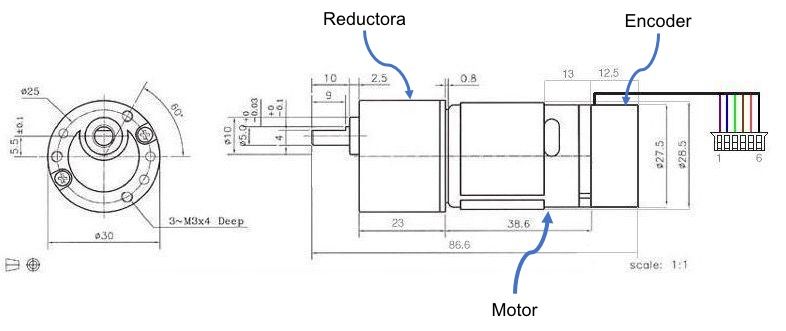
\includegraphics[width=\textwidth]{esquema_motor.jpg}
\caption{Esquema del motor eléctrico EMG30}\label{f1}
\end{figure}
\subsection{El motor EMG30} \label{s111}
El EMG30 \cite{EMG30}, figura \ref{f1}, es un motor de continua de $12V$, equipado con un encoder en cuadratura y una reductora que trasfiere al eje  externo una vuelta por cada 30 que da el eje principal. Examinaremos cada uno de estos elementos por separado.

\begin{table}
\centering
\begin{tabular}{r l r l}
\multicolumn{2}{c}{\textbf{Características del motor}}&\multicolumn{2}{c}{\textbf{Código colores cables}}\\
\hline
Voltaje Nominal & $12 V.$ & Morado (1) & Encoder B, Vout\\
Par Nominal  & $1.5 Kg\cdot m$& Azul (2) & Encoder A, Vout\\
Velocidad Nominal &  $170r.p.m$& verde (3) & Tierra Encoders\\
Intensidad Nominal & $530 mA$& Marrón (4) & Vcc Encoders (3.5v a 20v)\\
Velocidad sin Carga & $216r.p.m$& Red (5) & V$+$ Motor\\
Intensidad sin Carga & $150mA$ & Negro (6) & V$-$ Motor\\
Intensidad bloqueado&$2.5A$\\
Pontencia Nominal &$4.22W$\\
Pulsos encoder por vuelta del eje externo & 360\\
\hline
\end{tabular}
\caption{Motor EMG30}\label{t1}
\end{table}

\paragraph{Motor:}
Se trata de un motor de corriente continua, alimentado mediante escobillas. Las características fundamentales se describen en la tabla \ref{t1}. El motor está pensado para trabajar a un voltaje nominal de 12 V. En la práctica tomaremos dicho voltaje como el valor máximo admisible. Para alimentar el motor emplearemos una controladora que permite variar el voltaje nominal recibido por el motor en el rango $0-12V$ y cuya descripción general se dará más adelante. La figura \ref{f2} muestra una vista general del motor.
\begin{figure}
\centering
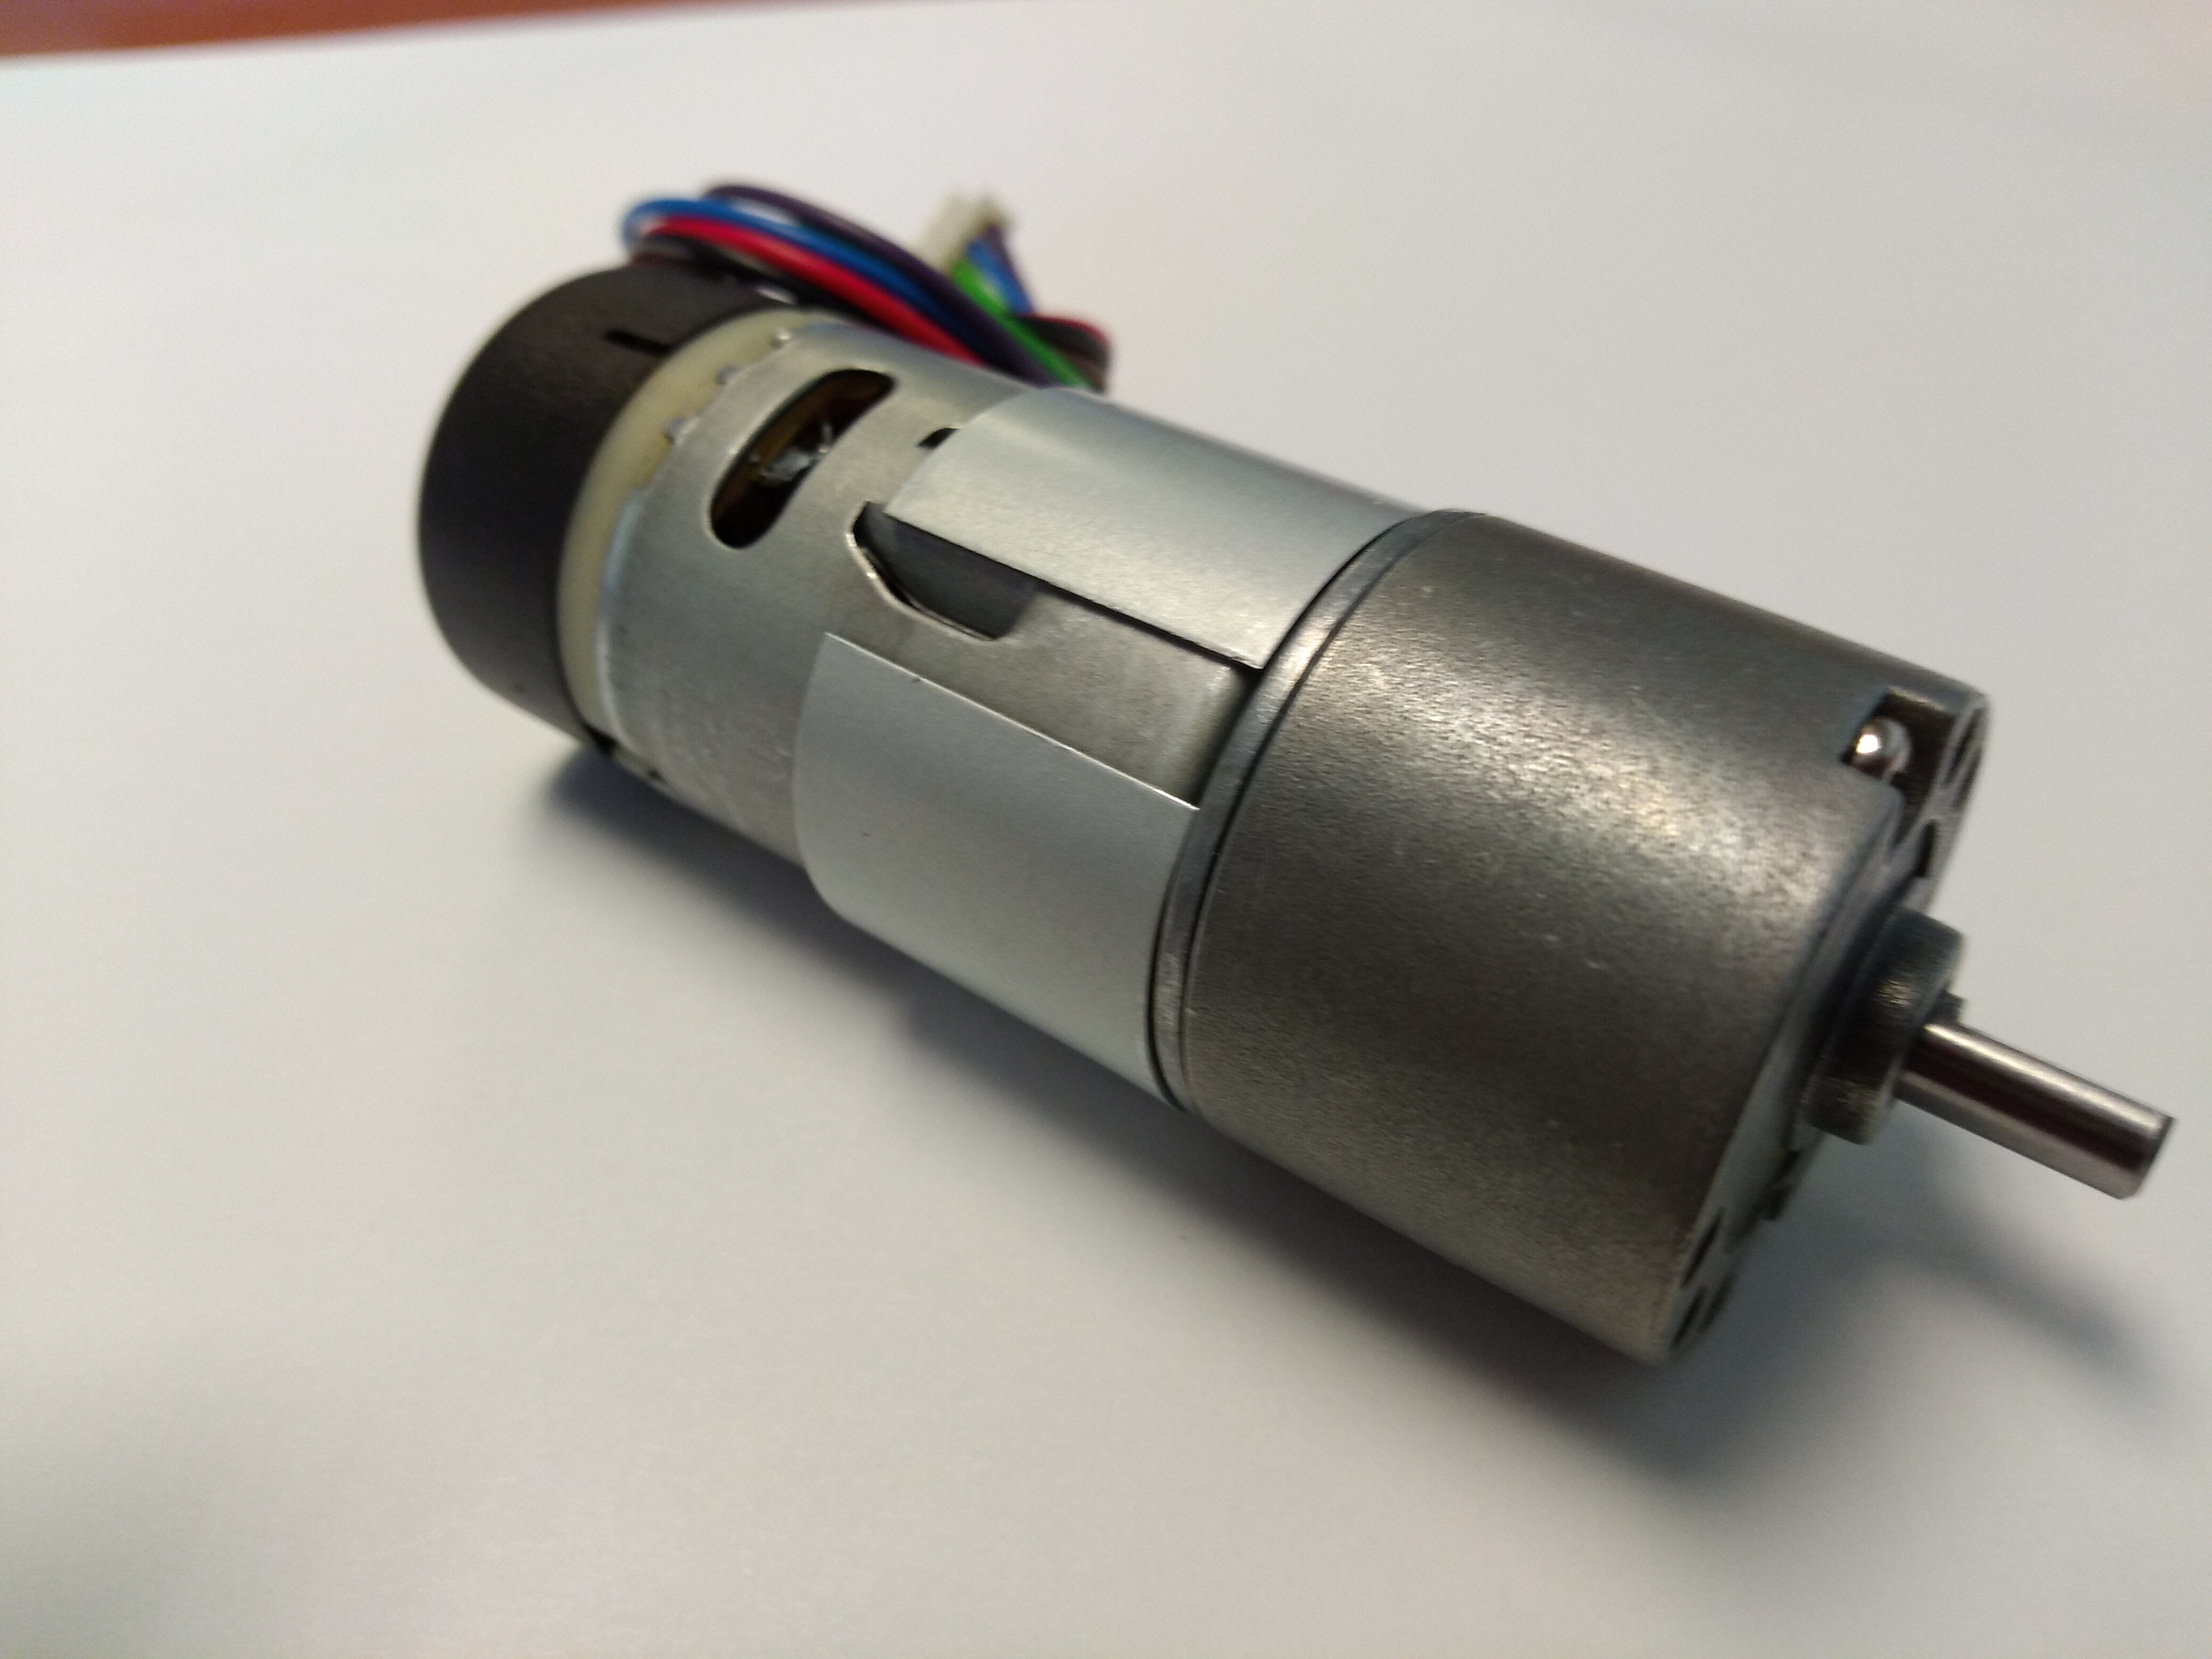
\includegraphics[width=0.5\textwidth]{emg30.jpg}
\caption{Motor eléctrico EMG30}\label{f2}
\end{figure}

\paragraph{Reductora}
El eje exterior del motor no coincide con el eje de su rotor. Ambos están conectados entre sí por un juego de ruedas dentadas que permiten desmultiplicar o reducir el número de vueltas. La relación de vueltas entre el eje del rotor y el eje exterior es de $30:1$, es decir el rotor da 30 vueltas por cada vuelta que observamos en el eje exterior. La reducción en velocidad que supone esta transformación lleva inmediatamente asociado un aumento del par mecánico. Es fácil comprobar este efecto sin más que tratar de girar el eje exterior del motor con la mano y observar la resistencia que ofrece. La figura \ref{f3} muestra una vista parcial del mecanismo de la reductora.

\begin{figure}
\centering
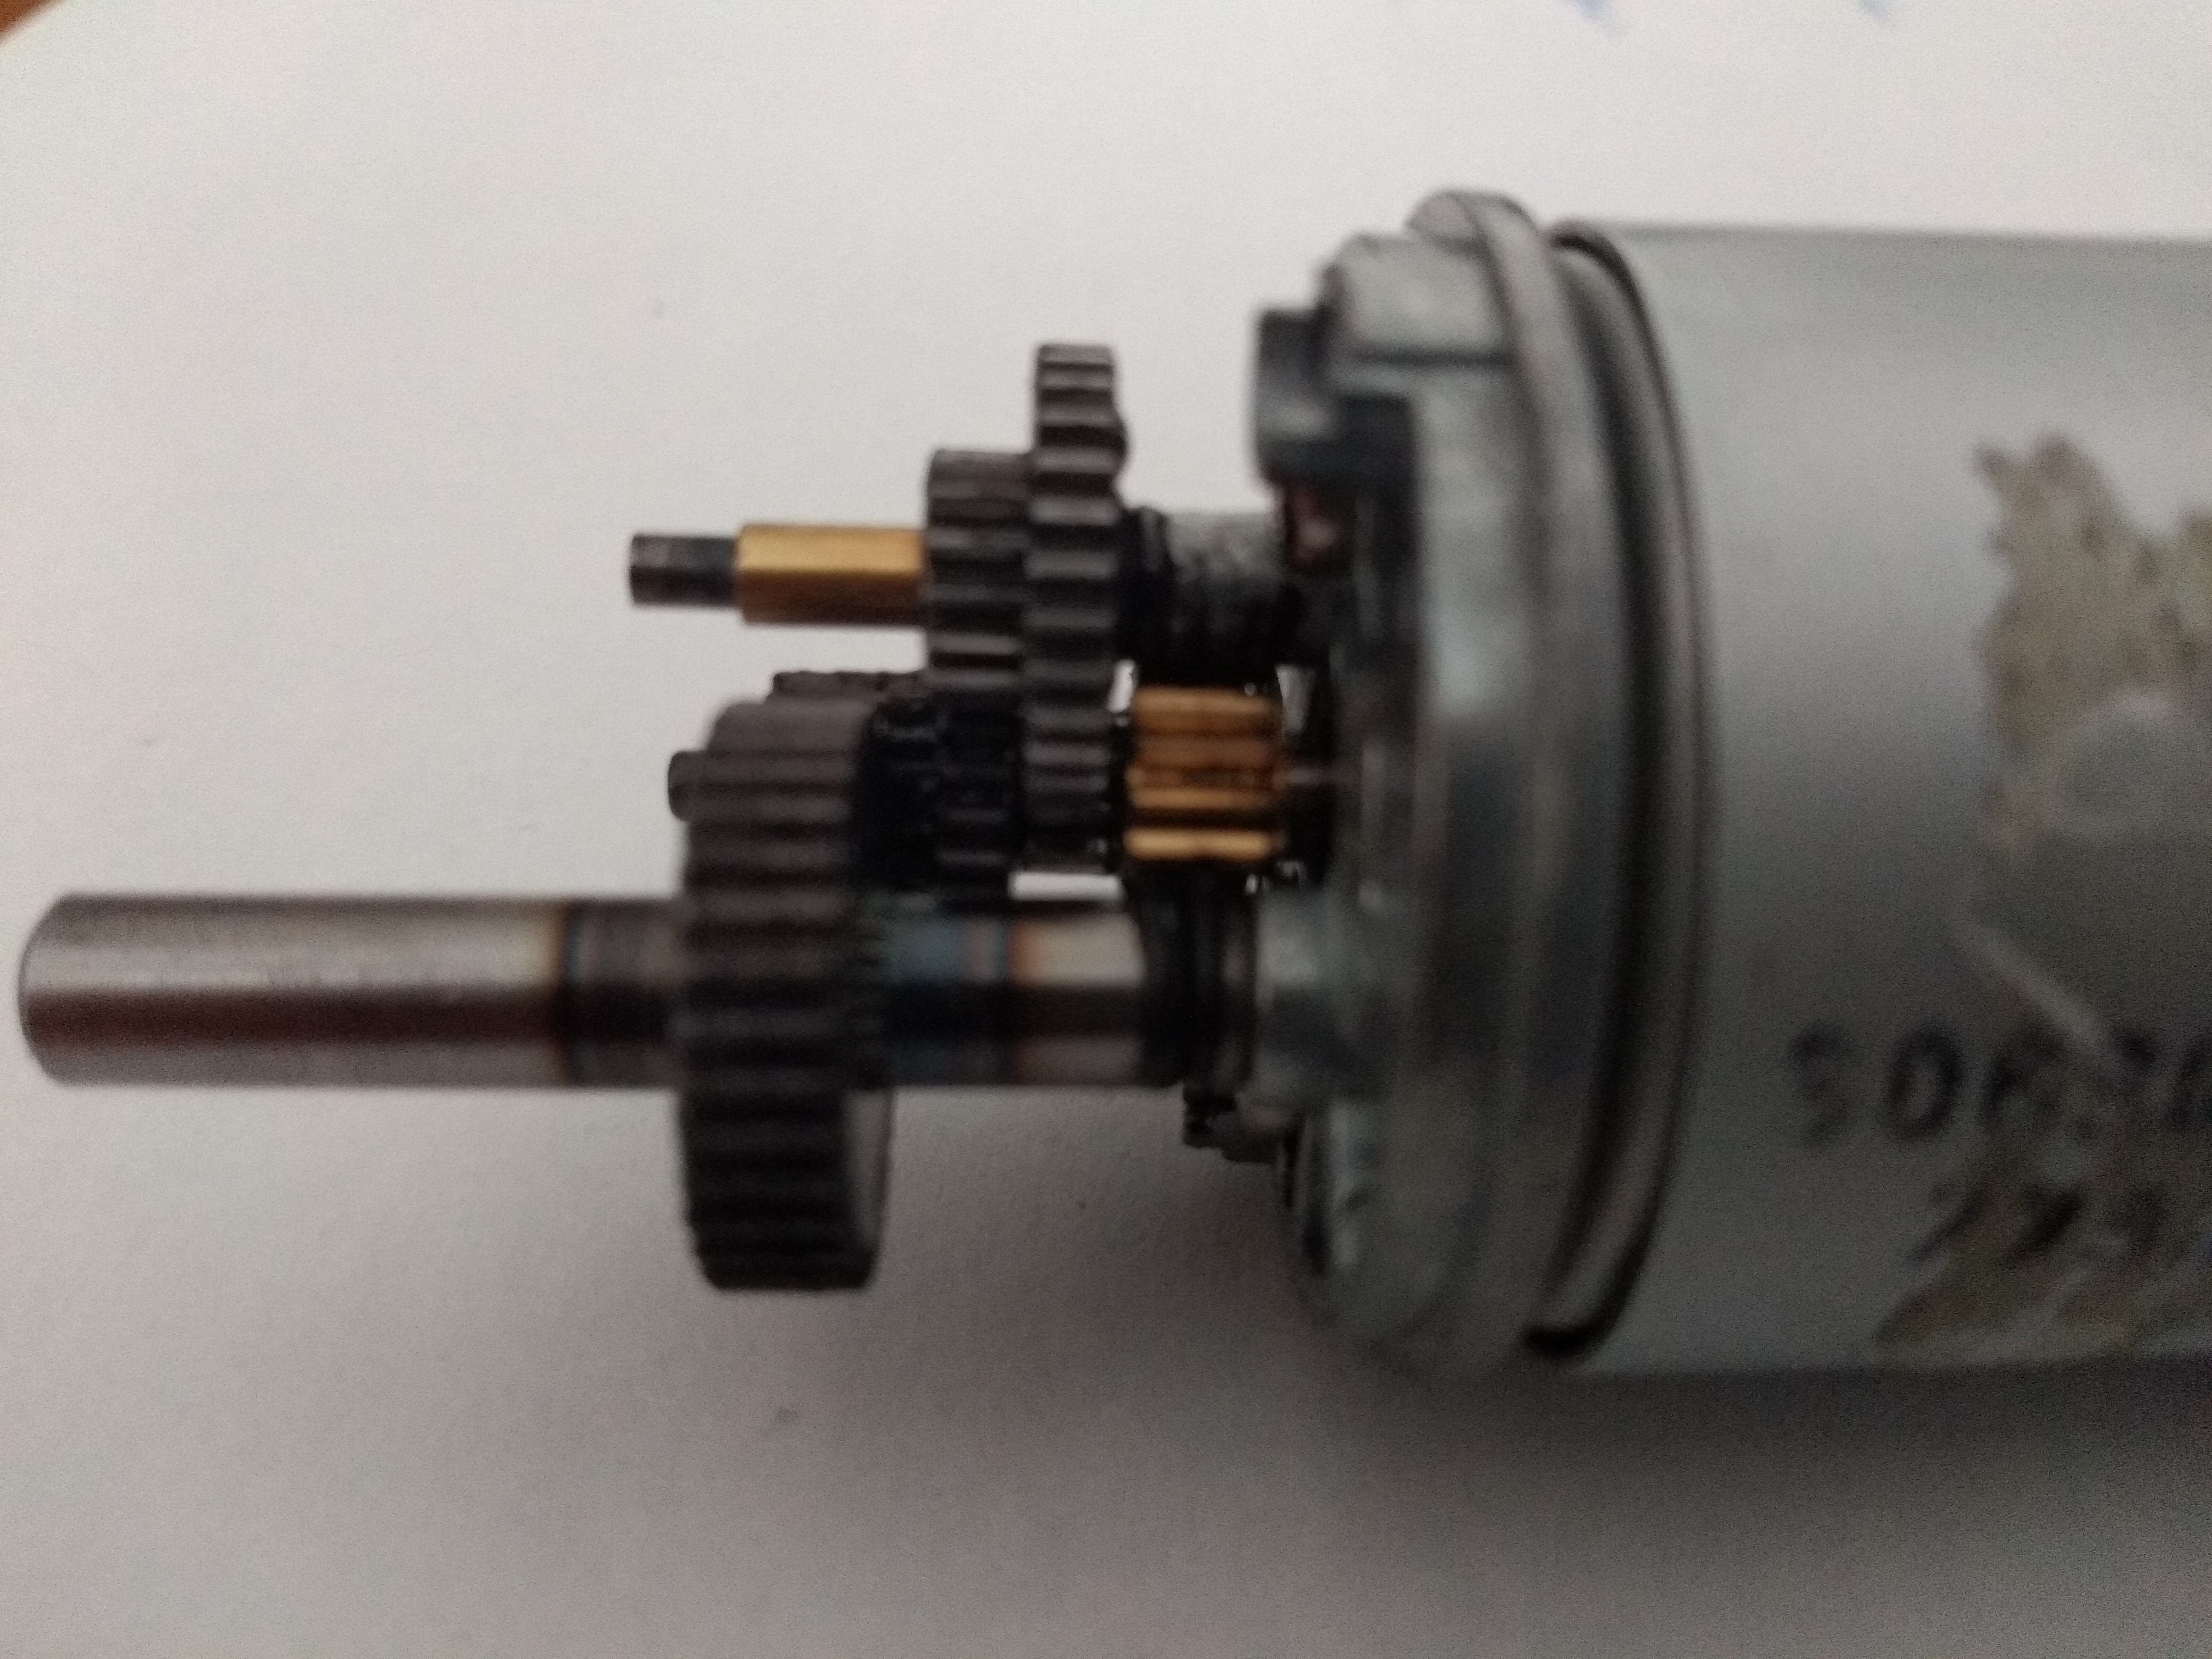
\includegraphics[width=0.45\textwidth]{red1.jpg}
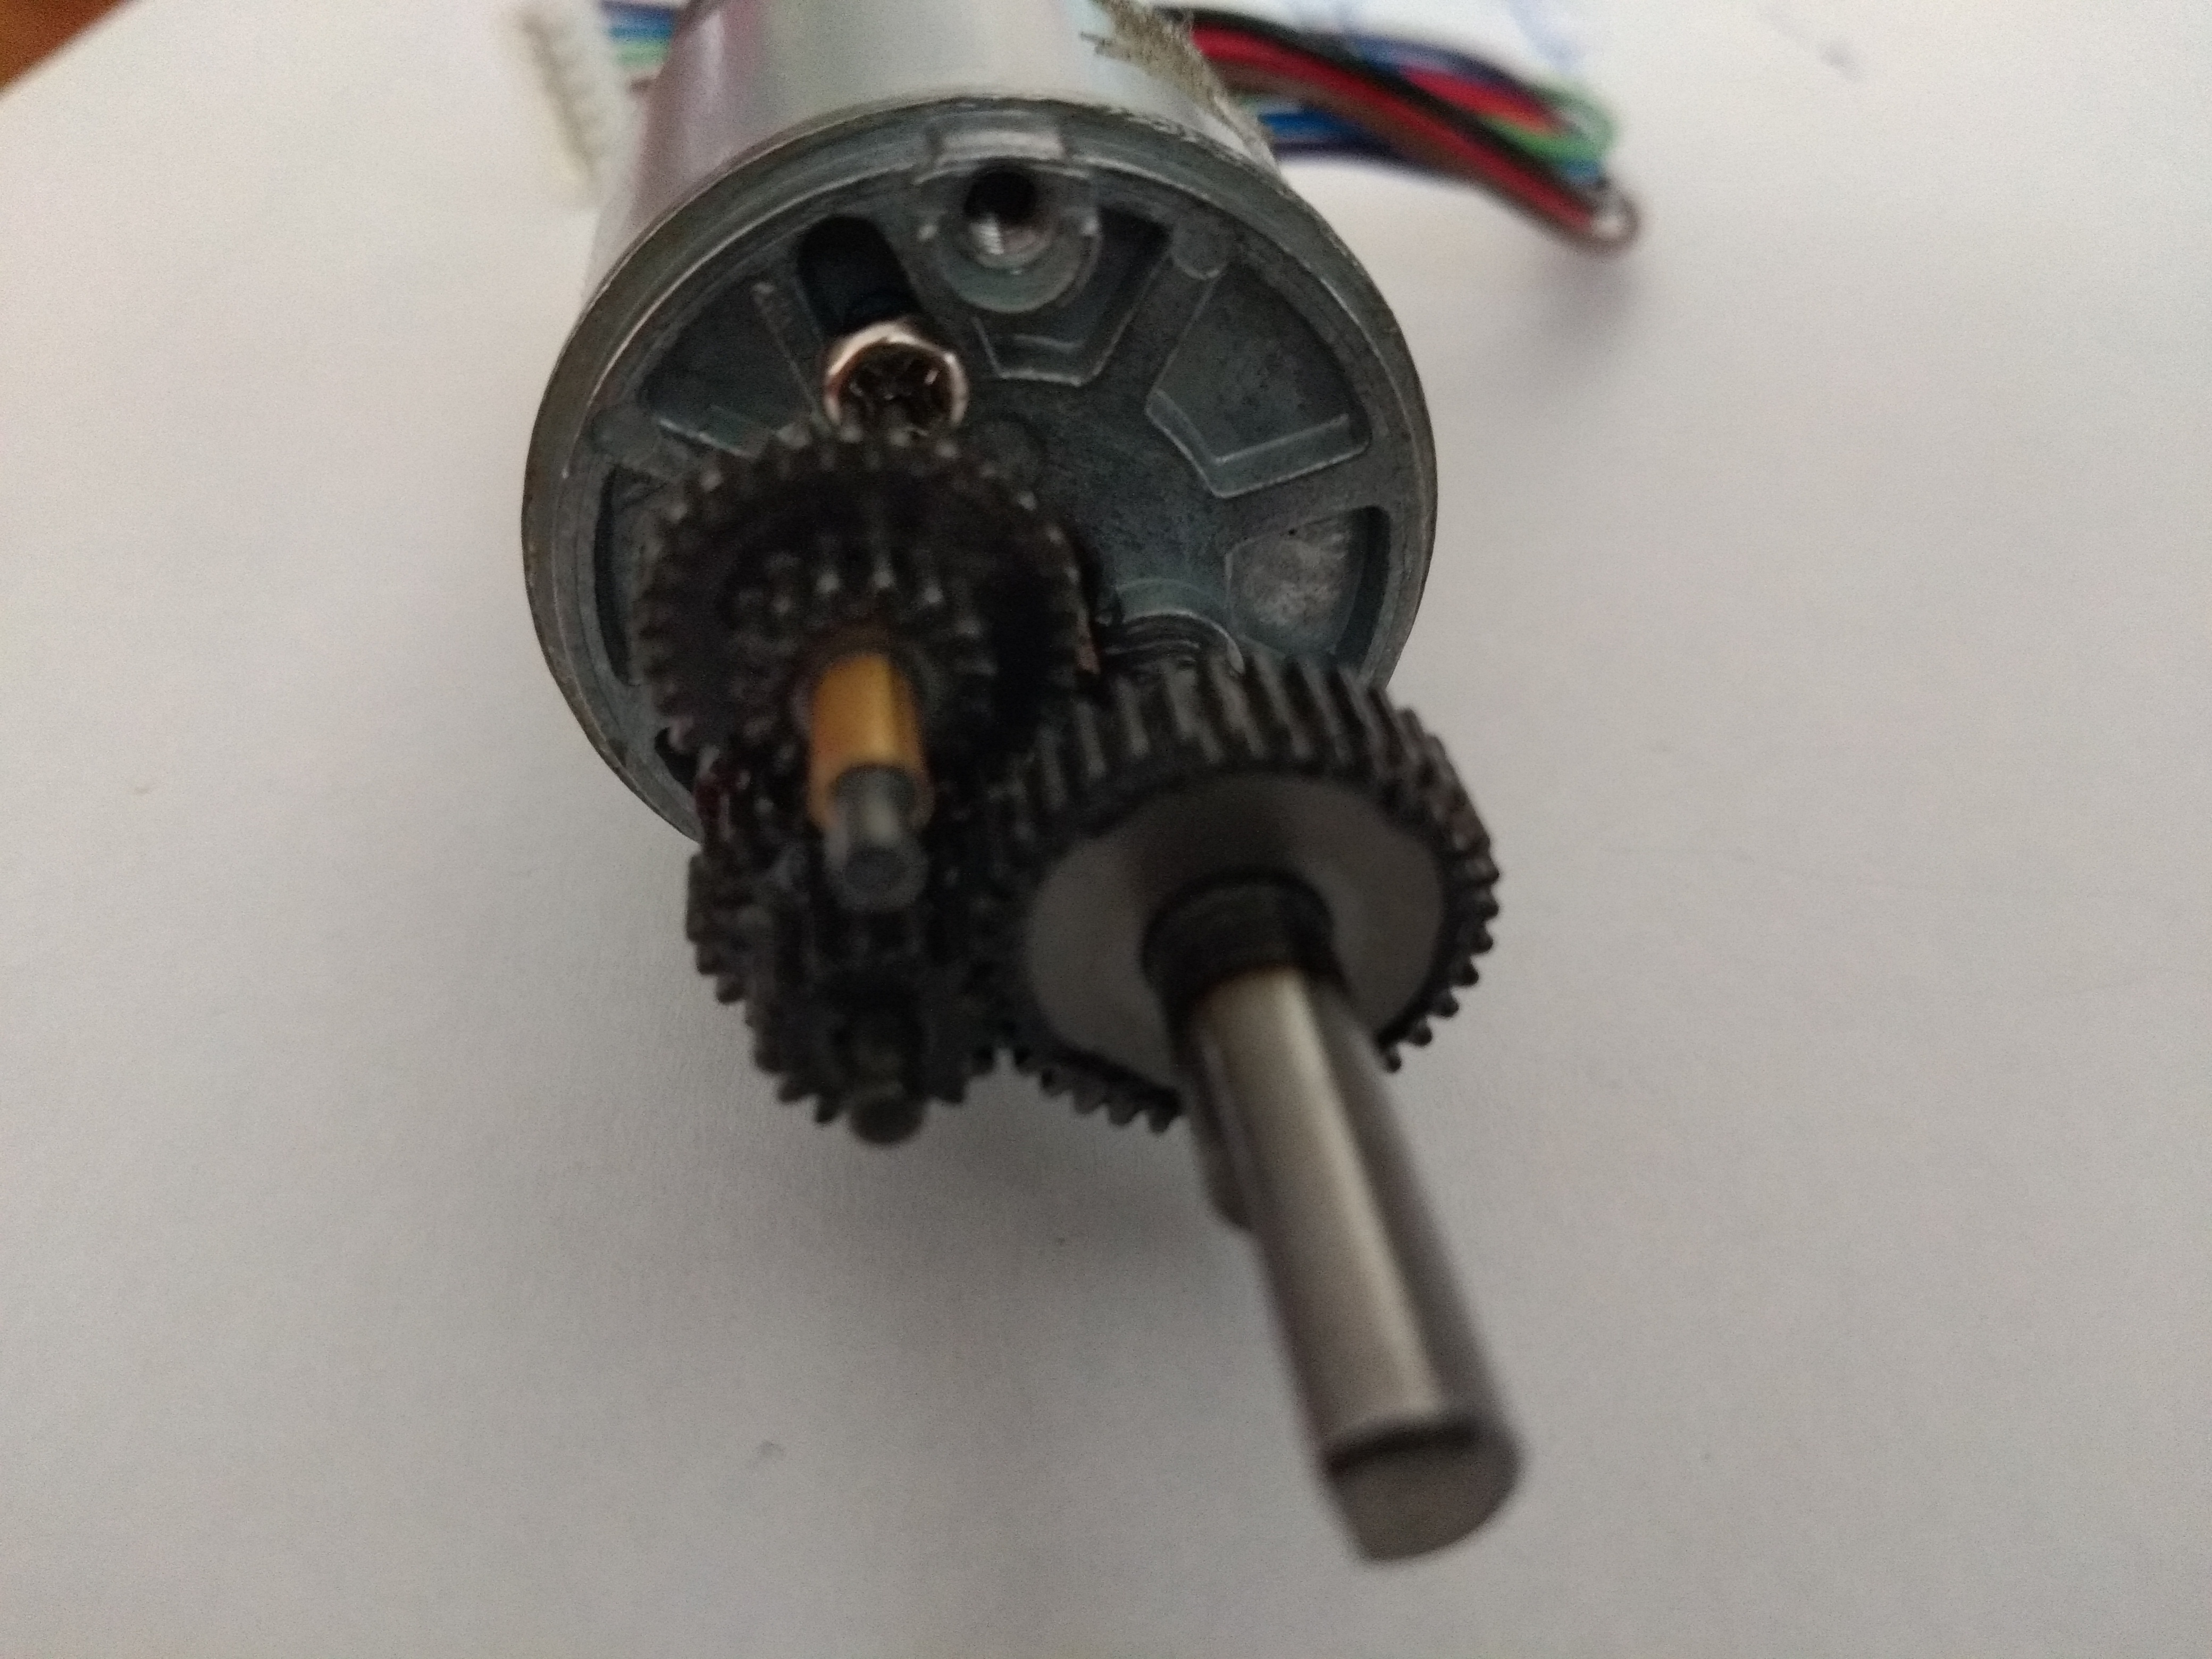
\includegraphics[width=0.45\textwidth]{red2.jpg}
\caption{Vistas parciales del mecanismo de la reductora}\label{f3}
\end{figure}

\paragraph{Encoder}
Este elemento, situado en la culata del motor, nos permite conocer el ángulo recorrido por el eje del motor. Se trata de un encoder en cuadratura de efecto Hall.
En general, un encoder es un dispositivo que permite conocer la posición de un mecanismo, mediante la lectura de pulsos. En nuestro caso, los pulsos los produce un juego de imanes permanentes, situados en el eje del motor, al excitar un par de sensores de efecto Hall.
La figura \ref{f4} Muestra una vista del  encoder situado en la culata del EMG30. El disco central unido al eje contiene los imanes y, por traterse de un encoder en cuadratura, tiene dos sensores de efecto Hall situados a $90^o$ el uno del otro.
\begin{figure}
\centering
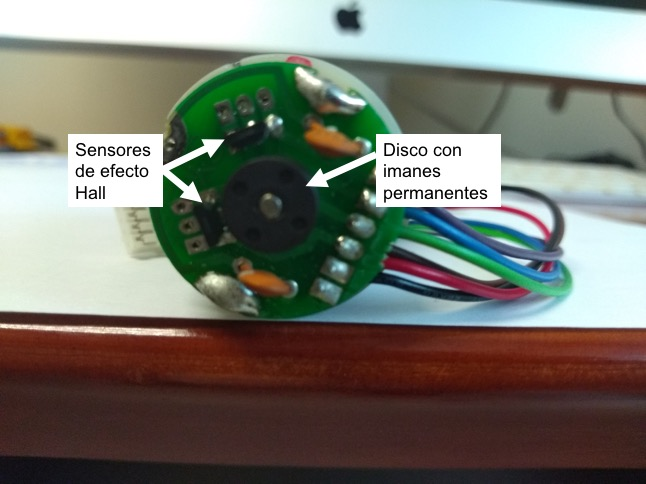
\includegraphics[width= 0.7\textwidth]{encoder1.jpg}
\caption{Vista del encoder situado en la culata del motor EMG30}\label{f4}
\end{figure} 

Si nos fijamos en el funcionamiento de uno de los sensores de efecto Hall, cada vez que uno de los imanes del disco del eje, pasa por delante del sensor, este se excita produciendo un nivel de tensión alto, cuando el imán deja de excitar al sensor, éste dará un valor de tensión bajo (equivalente a cero). Si el motor esta girando, la señal emitida por el sensor será una onda cuadrada, correspondiente a los niveles altos y bajos de voltaje descritos. La figura \ref{f5} muestra un ejemplo de la onda generada. Como los imanes permanentes están distribuidos uniformemente entorno al eje del motor, es suficiente con conocer su número para conocer cuánto ha girado el motor. Así, por ejemplo si tenemos tres imanes cada uno cubrirá un rango de $120^o$ por tanto si contamos los flancos de subida de la señal producida y multiplicamos por $120^o$, podemos calcular los grados que ha avanzado el motor y si dividimos entre tres, podemos calcular el número de vueltas que ha dado. Podemos refinar nuestras medidas un poco  más si contamos tantos los flancos de subida como los de bajada. En el ejemplo anterior de los tres imanes, la distancia entre dos flancos consecutivos (subida-bajada), (bajada-subida) será de $60^o$, con lo que si contamos todos los flancos duplicamos la sensibilidad de nuestro encoder.

Si usamos un solo sensor, como hemos descrito hasta ahora, nos encontramos con el problema de que no sabemos el sentido de giro del motor, ni podemos tampoco detectar los cambios de sentido de giro.
La solución a este problema se consigue con el segundo sensor de efecto Hall, que está situado de modo que sus flancos caen justo a mitad de los pulsos del primer encoder. El resultado de las señales de  ambos sensores  se muestra superpuesto en la figura \ref{f6}. 

\begin{figure}
\centering
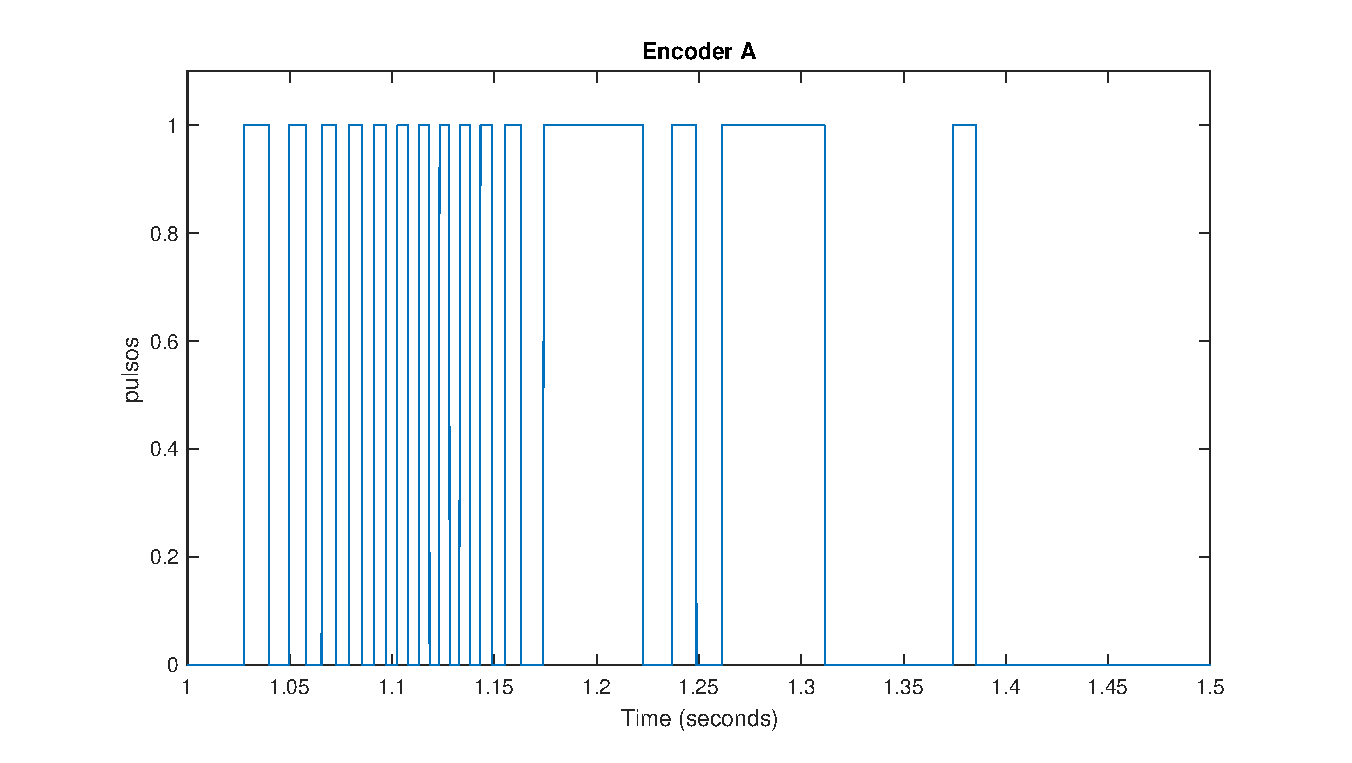
\includegraphics[width= 0.7\textwidth]{encodera.eps}
\caption{Señal producida en uno de los encoders (sensor de efecto Hall)al girar el motor }\label{f5}
\end{figure} 
Si tomamos como referencia el sensor marcado como encoder A (rojo en la figura), si el motor gira en un sentido, sus flancos de subida irán siempre seguidos por flancos de subida del encoder B, pero si gira  en sentido contrario entonces un flanco de subida de A irá seguido por un flanco de bajada de B. Además, cuando se de un cambio de sentido de giro observaremos dos flancos seguidos del mismo sensor. Dos sensores así dispuestos constituyen lo que se conoce con el nombre de encoder en cuadratura. Adicionalmente, hemos duplicado el número de flancos, por lo que ahora, la distancia entre flancos  es la mitad que para el caso de un solo sensor.
\begin{figure}
\centering
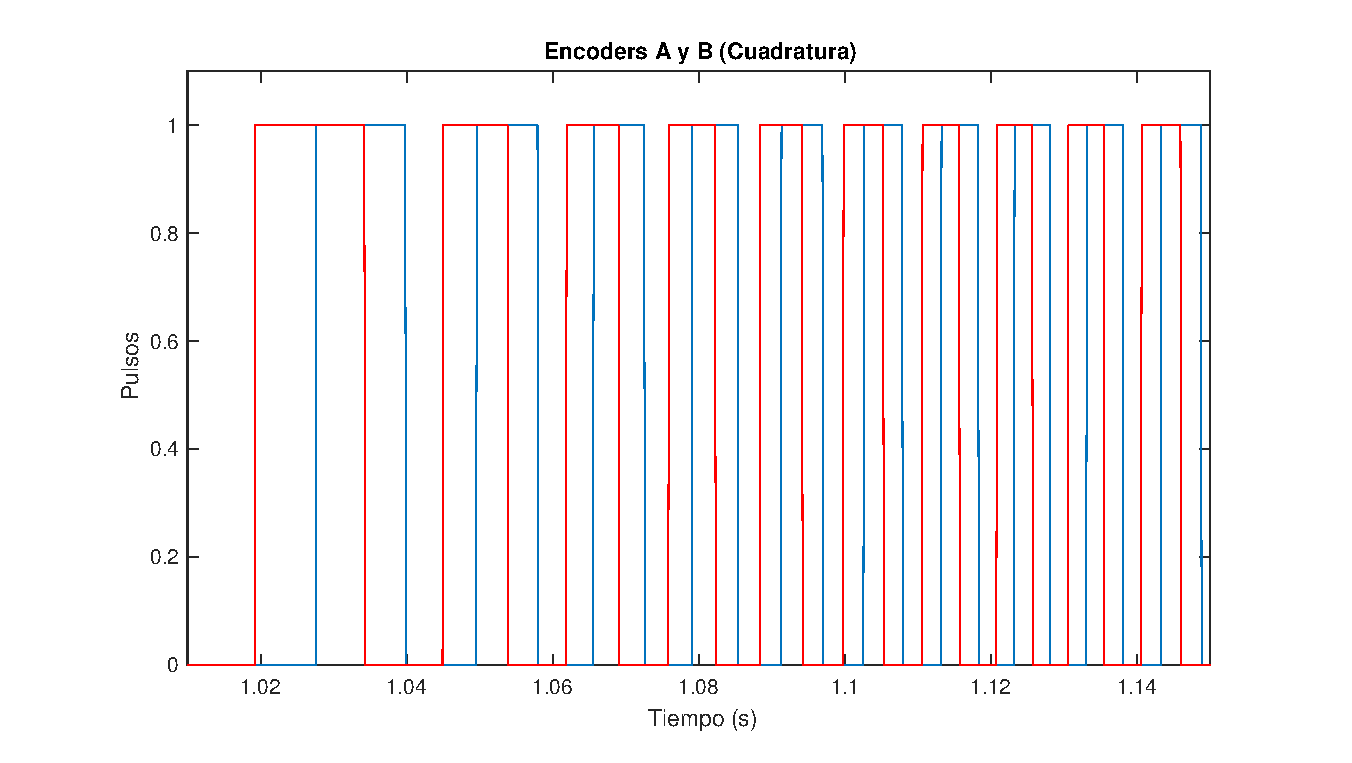
\includegraphics[width= 0.7\textwidth]{encoderab.eps}
\caption{Señales producidas por un encoder en cuadratura al girar el motor }\label{f6}
\end{figure} 

Si nos fijamos en las especificaciones de la tabla \ref{t1}, se indica que el encoder cuenta 360 pulsos por revolución del eje exterior del motor, cada pulso representa un cambio, es decir un flanco de subida o bajada en la señal. La distancia entre dos pulsos sería por tanto de un grado. Esa es la máxima resolución que permite el encoder. Podemos intentar a partir de este dato, deducir la configuración del encoder. Sabemos que la relación de la reductora es 30:1, por tanto el eje del motor da 30 vueltas por cada una de las del eje exterior. Si dividimos el número de pulsos entre el de vueltas del eje principal obtenemos $360/30 = 12$ Es decir el encoder cuenta 12 pulsos por cada vuelta del eje del motor. Como tenemos dos sensores, cada uno de ellos deberá contar seis pulsos,  Tres de ellos corresponderán a flancos de subida (s) y tres a flancos de bajada (b) s-b-s-b-s-b. Por tanto podemos deducir que, por cada vuelta del eje, cada sensor se ha excitado tres veces, lo que corresponde a tres imanes equiespaciados en el disco giratorio situado en torno al eje. Cada imán excita al sensor cubriendo un ángulo de $60^o$, entre los imanes hay una zona \emph{muerta} que cubre también un ángulo de $60^o$. La disposición de los sensores, situados a $90^o$, explica su funcionamiento en cuadratura: Cuando un imán está centrado en un sensor, el siguiente imán esta empezando a excitar al siguiente sensor, o acaba de excitar al anterior, dependiendo del sentido de giro. La figura \ref{f7} muestra esquemáticamente este resultado.

\begin{figure}
\centering
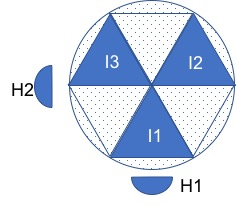
\includegraphics[width= 0.5\textwidth]{esqhall.jpg}
\caption{Esquema de la posición relativa de los sensores de efecto Hall (H1 y H2) y los imanes permanentes para el encoder del motor EMG30. En la posición que se muestra, H2 estaría en un flanco e subida o bajada --según la dirección de giro del motor-- y H1 Estaría en en centro de un pulso}\label{f7}
\end{figure} 

\subsection{La controladora del motor}\label{sh}
Para un motor de corriente continua, la velocidad de giro del motor está directamente relacionada con la tensión a la que alimentemos sus terminales eléctricos. Además el sentido de giro vendrá determinado por la polaridad de la fuente de alimentación. Si invertimos la polaridad de los terminales, el motor invierte su sentido de giro. Podemos por tanto variar tanto el sentido de giro como la velocidad. Analicemos por separado ambas posibilidades.

\paragraph{Variación del sentido de giro: Puente en H.}
Para controlar el sentido de giro del motor es habitual emplear un circuito conocido como puente en H. La figura \ref{f8} muestra el esquema de un puente en H, construido a partir de transistores. La configuración del circuito, --con el motor situado en el centro de una H formado por los cuatro transistores-- es la que da origen a su nombre.

El funcionamiento es sencillo de entender: los transistores actúan como interruptores de modo que si suministramos una tensión de referencia a las puertas G1 y G4 manteniendo a tierra G2 y G3, circulará corriente entre $V+$ y tierra, cruzando el motor desde el terminal izquierdo al derecho, haciendo girar al motor en un sentido. Si, por el contrario, damos tensión a G2 y G3, manteniendo G1 y G2 a tierra, la corriente atravesará el motor desde el terminal derecho al izquierdo, haciendo girar el motor en sentido contrario. Los diodos tiene por objeto proteger el motor durante la conmutación de una situación a otra\footnote{El funcionamiento real y el papel de los diodos es un poco más complejo. Aquí solo se han expuesto las ideas más básicas.}. 
\begin{figure}
\centering
\begin{circuitikz}
\draw(0,0.5)node[nigfete](nigfete3){};
\draw(5,0.5) node[nigfete,xscale = -1 ](nigfete4){};
\draw(0,2) node[nigfete](nigfete1){};
\draw(5,2) node[nigfete,xscale = -1](nigfete2){};
\draw(nigfete1.D)--(nigfete2.D);
\draw(nigfete3.S)--(nigfete4.S);
\draw(nigfete1.G)node[anchor=east]{G1};
\draw(nigfete2.G)node[anchor=west]{G2};
\draw(nigfete3.G)node[anchor=east]{G3};
\draw(nigfete4.G)node[anchor=west]{G4};

\draw (1,1.2)to[/tikz/circuitikz/bipoles/length=0.5cm,D*](1,2.8);
\draw (4,1.2)to[/tikz/circuitikz/bipoles/length=0.5cm,D*](4,2.8);
\draw (1,-0.3)to[/tikz/circuitikz/bipoles/length=0.5cm,D*](1,1.2);
\draw (4,-0.3)to[/tikz/circuitikz/bipoles/length=0.5cm,D*](4,1.2);
\draw (0,1.2) to[sV, color=white, name=M2] (5,1.2);
\mymotor{M2}{0}

\draw(2.5,2.77)to[short,-*](2.5,3.5)node[anchor=west]{$V+$}(2.5,3.5);
\draw(2.5,-0.3)--(2.5,-1)node[ground]{};
\end{circuitikz}
\caption{Esquema del circuito de un puente en H}\label{f8}
\end{figure}

\paragraph{Variación de la velocidad: Señal de PWM.}
Como se ha indicado antes, la velocidad a la que gira un motor de continua varía directamente con el voltaje suministrado. Es más, en un cierto rango de voltaje, y dependiendo del tipo de carga a que esté sometido, se puede considerar que velocidad y voltaje son proporcionales. Podemos por tanto variar la velocidad del motor si somos capaces de variar el voltaje suministrado.

Un método frecuente de hacerlo es emplear una señal de PWM. Las siglas PWM provienen del Inglés \emph{Pulse Width Modulation} (Modulación por Ancho de Pulso). La figura \ref{f9} Muestra un ejemplo de una señal PWM.
La señal tiene tres parámetros característicos importantes. 
El valor máximo de la señal; en el ejemplo de la figura sería $V_{max}=10V$. El periodo $T$, que  define el tiempo transcurrido entre dos flancos de subida. Habitualmente, el periodo suele definirse en función del tiempo de respuesta del sistema y se procura que sea significativamente bajo respecto a éste. En el caso del ejemplo mostrado en la figura \ref{f9} $T=1 ms$. Por último, el Ciclo activo \emph{Duty Cicle} $\Delta T$, que corresponde al periodo durante el cual la señal de PWM está activa y alcanza su valor máximo. En el ejemplo de la figura \ref{f9} $\Delta T\approx 0.2 ms$.

\begin{figure}
\centering
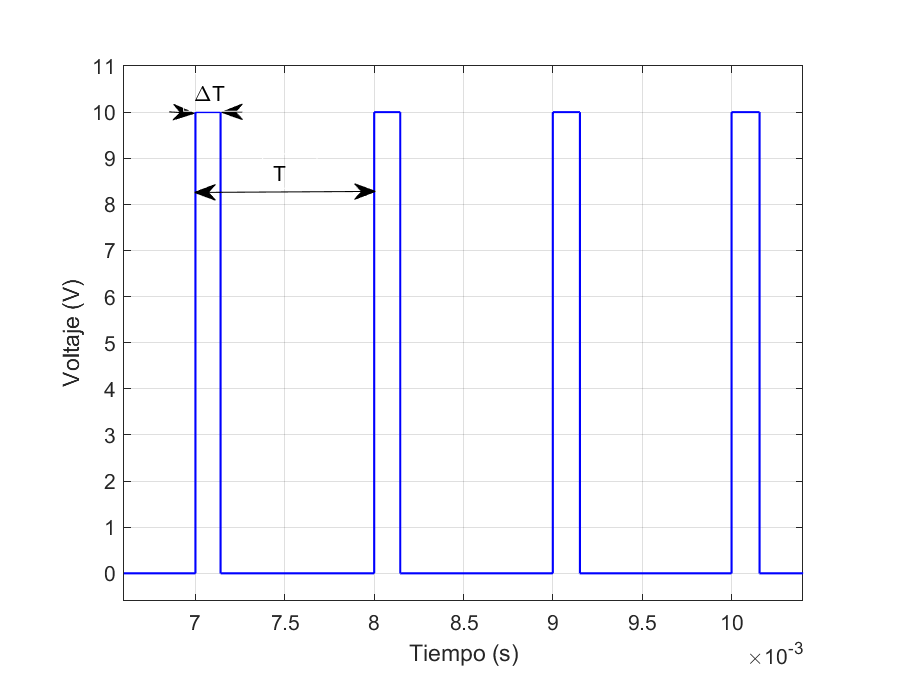
\includegraphics[scale=0.7]{pwm.eps}
\caption{Señal de PWM}\label{f9}
\end{figure} 

Supongamos que hacemos llegar una señal de PWM a las Puertas G1 y G4 del puente en H de la figura \ref{f6}. Los transistores abrirán el puente durante el \emph{duty cicle} de modo que el motor recibirá corriente solo durante dichos periodos de tiempo. Sin embargo el tiempo de respuesta de un motor es, por lo general superior al periodo $T$ de la señal, por lo que no podrá arrancar y parar al ritmo de ésta. El resultado es que es motor \emph{filtrará la señal} quedándose con su valor medio. Si lo calculamos para un ciclo,
\begin{equation}
\frac{1}{T}\int^T_0 V_{PWM}dt = \frac{1}{T}\left(\int^{\Delta T}_0 V_{+}dt 
+ \int^{T}_{\Delta T} 0 dt\right)) = \frac{\Delta T}{T}V_{+}
\end{equation}

El motor estaría  \emph{viendo} una tensión que equivaldrá al valor de la tensión de la fuente $V+$ multiplicada por la relación entre el \emph{duty cicle} y el periodo de la señal de PWM. Si modificamos el \emph{duty cicle} entre $0$ y $T$, El voltaje variará entre $0$ y $V+$.

\paragraph{El controlador X\_NUCLEO\_IHM15A1} Para controlar el motor emplearemos una placa con un microcontrolador junto con  la placa de expansión X\_NUCLEO\_IHM15A1 fabricada por la compañía ST \cite{IHM15}. Dicha placa emplea el circuito integrado  STSPIN840  \cite{STSPIN840} que contiene dos puentes en H y todos los dispositivos necesarios para la manipulación y protección de los mismos. A su vez, la placa viene preparada para su conexión directa con las Placas STM32 Nucleo que, como se verá más adelante emplearemos tanto para generar las señales de PWM como para registrar las lecturas de los encoders y controlar el comportamiento del motor. La figura \ref{f10}, muestra una imagen de la placa. 

Entre las característica principales de la placa, resalta que admite voltajes de entrada entre $7V$ y $45V$, para corrientes de hasta $1.5 A$ por fase. Como se ha indicado anteriormente, el circuito contiene dos puentes en H, marcados como puente A y puente B.  En principio en la placa se puede configura  cada puente por separado, o los dos puentes juntos. De este modo, se podría suministra corriente a dos motores, con posibilidad de invertir su sentido de giro, o a un solo motor también con la posibilidad de invertir su sentido de giro. En nuestro caso, emplearemos  una configuración en la que alimentaremos un solo motor empleando los dos puentes a la vez, de este modo podemos suministrar una corriente al motor de hasta $3 A$.  

Pero antes de seguir adelante, examinemos la figura \ref{f10}. En la parte superior de la imagen ---tal como se ha representado-- encontramos una foto de la placa con un conector verde con seis tomas. De abajo arriba, la primera es una entrada, marcada como $GND$ que debe conectarse al terminal negativo de la fuente. Corresponde a la \emph{tierra} o referencia de voltaje $0$. La segunda toma $V_{s}$ es la entrada de voltaje, debe conectarse al terminal positivo de la fuente que se empleará para alimentar el motor. Para el caso de nuestro motor debería conectarse al terminal positivo de una fuente de $12V$ como máximo, puesto que ésta es la tensión nominal del motor (ver sección \ref{s111}). Representaría la entrada correspondiente al voltaje $V+$ del puente en H (fig.\ref{f8}).  Las tomas tercera y cuarta son salidas que suministran voltaje a través de uno de los puentes en H que contiene la placa. En concreto, se trata del puente A. Están marcadas con los símbolos $A1$ y $A2$. Por último las tomas quinta y sexta son las salidas de voltaje correspondiente al segundo puente de la placa --el puente B-- están Marcadas $B2$, $B1$.

Como se ha indicado anteriormente, en nuestro caso, vamos a usar ambos puentes a la vez para alimentar al mismo motor. Para ello,  (figura \ref{f10}) es preciso colocar el \emph{jumper} de modo paralelo \emph{Parallel mode jumper} en la posición PAR .Esto permite controlar a la vez los dos puentes con una sola señal para el sentido de giro y una sola señal de PWM.

Nuestro motor deberá ir conectado a la placa de modo de la salidas $V1$ tanto del puente A como del B estén conectadas al  cable rojo ($V+$) del motor y las salidas $V2$ estén conectadas al cable negro ($V-$) del motor. 

Por último debemos hablar de los pines de la placa desde los que controlaremos la dirección y la velocidad del motor. Se trata de las entradas lógicas de la tarjeta.  En el esquema de la figura \ref{f10}, se han marcado cuatro pines. Los dos en rojo ENA y ENB, Habilitan el puente en H A y el puente en H B, respectivamente. Ambos deberán recibir un $1$ lógico desde las correspondientes salidas de la placa del microcontrolador (ver sección \ref{sec_mic}). El pin marcado en azul PWMA representa la entrada de la señal de PWM necesaria para controlar el puente A. Dado que hemos colocado el \emph{jumper} en la posición paralelo, esta señal activará a la vez tanto al puente A como al puente B. Esta señal será tambien enviada desde la placa del microcontrolador. 
\begin{figure}
\centering
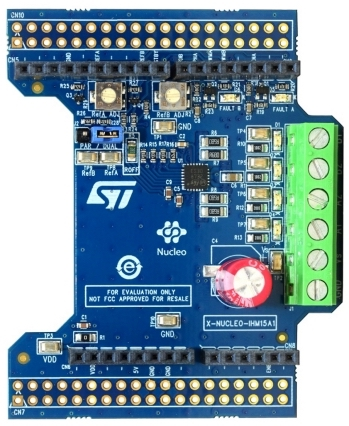
\includegraphics[scale=0.65]{IHM15A1.jpg}

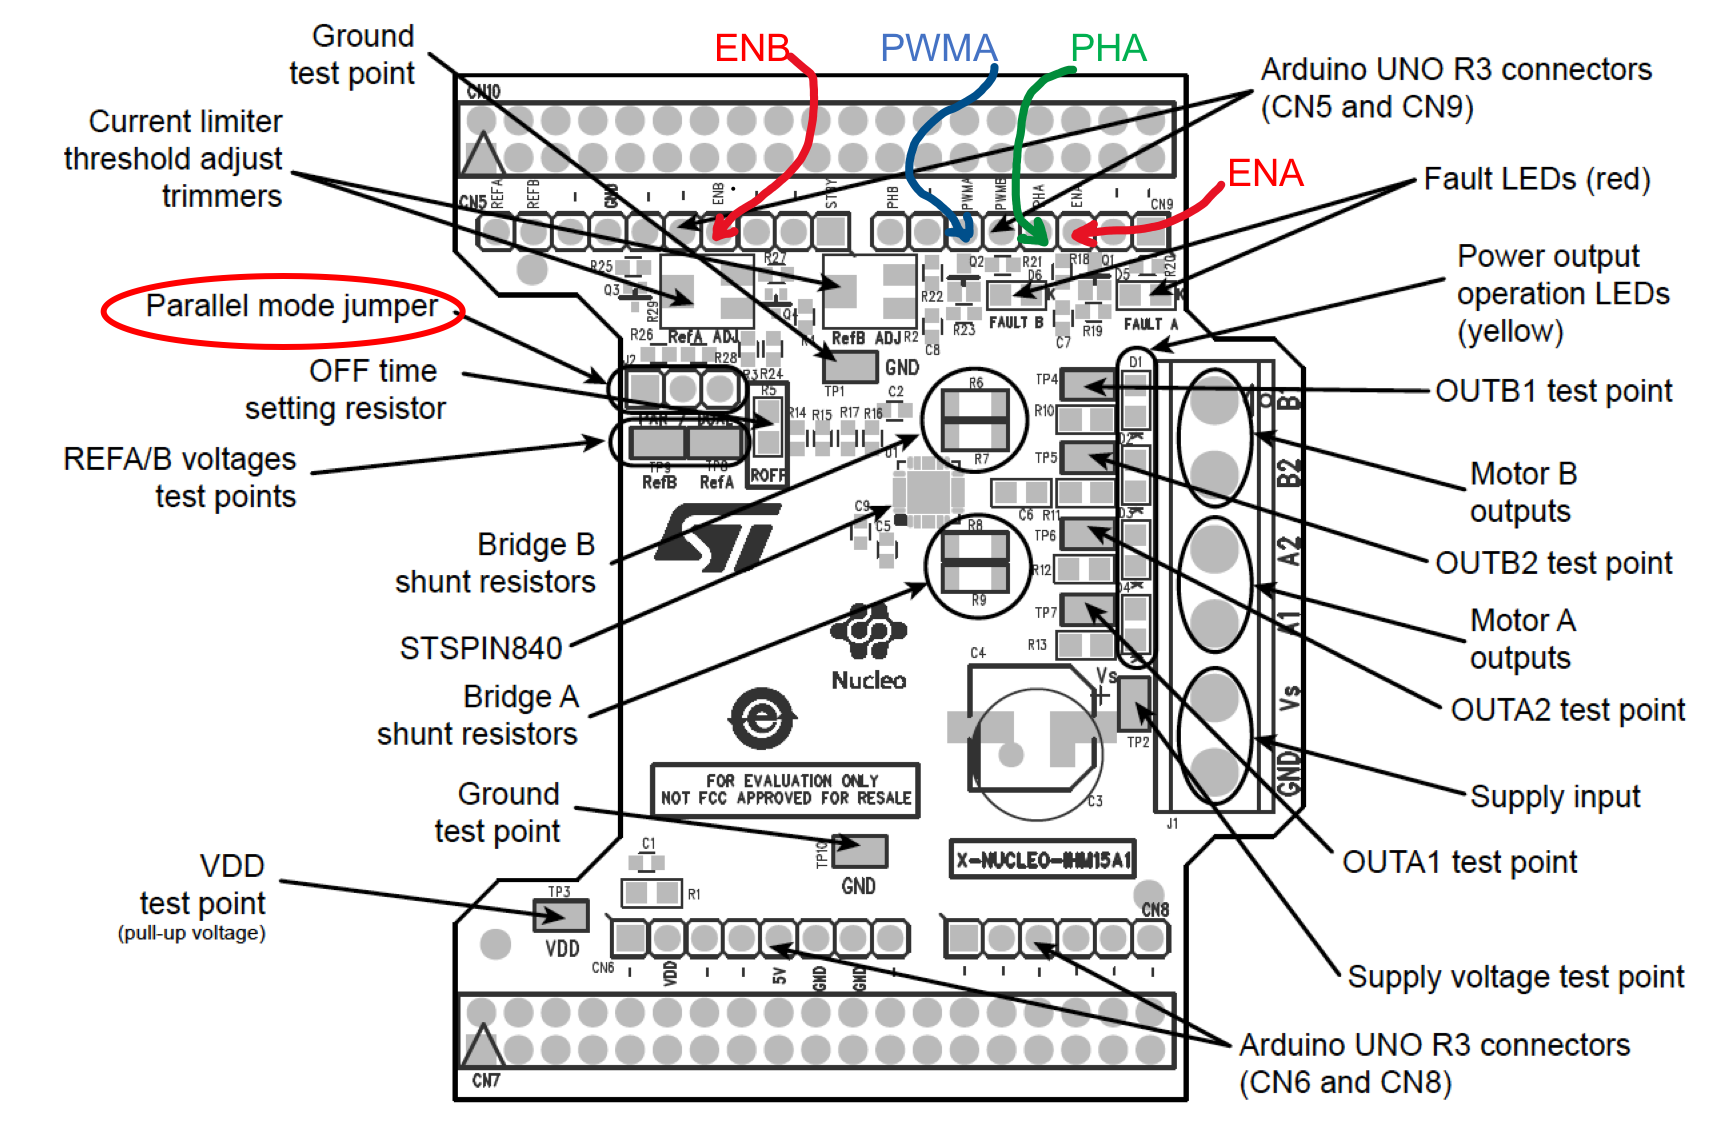
\includegraphics[scale=0.55]{IHM15A1E1.png}
\caption{Placa de expansión, X-NUCLEO-IHM04A1}\label{f10}
\end{figure}
Por último, la entrada marcada en verde como PHA, permite cambiar el par de puertas G1-G4 ó G2-G3 por las que se introduce la señal de PWM, cambiando de este modo el sentido de giro del motor. Para hacerlo girar en un sentido, debemos enviar desde la salida correspondiente de la placa del microcontrolador un $0$ lógico, para invertir el sentido de giro, deberemos enviar un $1$.

La placa de expansión presenta más opciones de configuración que no emplearemos en estas prácticas. Los interesados en saber más, pueden recurrir a las hojas de características incluidas en la bibliográfia

  
\subsection{El microprocesador} \label{sec_mic}
El siguiente paso es generar las señales de control necesarias para alimentar  los pines lógicos de la placa que acabamos de describir. Para ello emplearemos la placa de desarrollo  Nucleo-411re STM32 fabricada por la compañía STMicroelectronics. El corazón de la placa es el microcontrolador STM32F411RE, un ARM cortex M-4.   
La  figura \ref{f11} muestra una imagen de  la misma. En dicha imagen, se pueden observar como la placa está dividida en dos partes. La parte de la derecha, antes de llegar a los botones azul y negro, es un programador, conocido como (ST-LINK), que permite introducir programas en la memoria del STM32F411RE, desarrollados en un ordenador normal y compilados mediante el uso de un compilador C/C++ cruzado. 
\begin{figure}
\centering
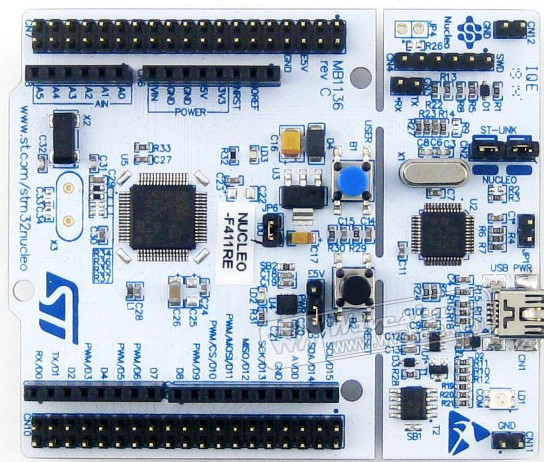
\includegraphics[scale=1.5,angle=180]{NUCLEO-F411RE.jpg}
\caption{Placa de desarrollo NUCLEO-F411RE }\label{f11}
\end{figure}
El programador se conecta al ordenador mediante el uso de un cable USB estándar. En el extremo de la placa se emplea un conector miniUSB. Además de permitir descargar código en el microcontrolador, el programador permite emular un puerto serie estándar, de modo que se puede emplear para enviar y recibir datos desde la placa al ordenador en tiempo de ejecución. También permite depurar código, aunque esta opción no la emplearemos en las prácticas. 

La parte de la izquierda de la placa, contiene el microcontrolador, un par de botones programables, un par de leds y el resto de la circuitería necesaria para hacer funcionar el microcontrolador. Además presenta dos juegos de pines (\emph{pin-outs}) distintos. El primero de ellos emula el \emph{pin-out} de la famosa placa de desarrollo de  Arduino. De este modo, hace posible conectar a la placa del microcontrolador cualquier placa de expansión compatible con la del Arduino. Se trata de los pines hembra que aparecen en la imagen de la figura \ref{f11}. El segundo juego de pines conocido como MORFO ofrece 64 pines macho.

En nuestro caso, emplearemos el \emph{pin-out} compatible con Arduino. Una de las razones para ello es que la placa de expansión que contiene los puentes en H para alimentar el motor, se inserta sobre  la placa de desarrollo, empleando dicho \emph{pin-out}. De este modo, podemos identificar rápidamente los pines empleados por la placa de expansión. Por su parte, la placa de expansión vuelve a replicar el \emph{pin-out} de Arduino, con lo que los pines no empleados por la placa de expansión quedan disponibles para otras aplicaciones.

La figura \ref{f12} muestra el esquema de conexiones del \emph{pin-out} de arduino, así como su nomenclatura.
\begin{figure}
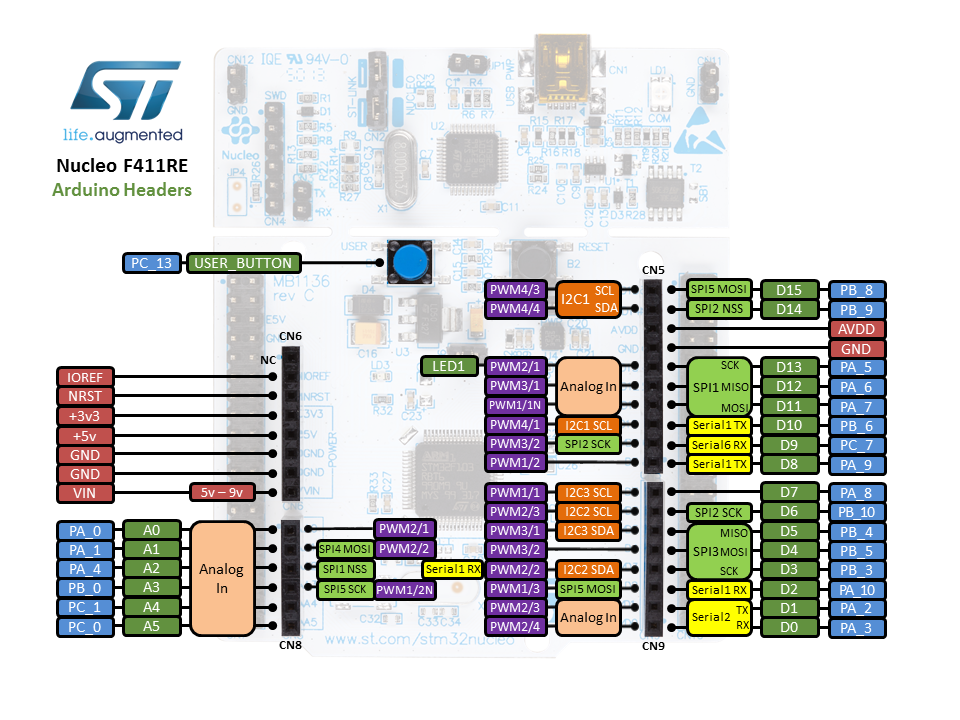
\includegraphics[scale=0.9,angle=90]{nucleo_f411re_arduino.png}
\caption{NUCLEO-F411RE. Pin-out compatible con Arduino, la nomenclatura es la de las etiquetas marcadas en verde}.\label{f12}
\end{figure}
Si nos fijamos, los pines están agrupados por conectores: CN5 con 10 pines, CN9 con 8 pines, CN6 con 8 pines y CN8 con 6 pines.
La placa de desarrollo empleada es bastante potente y versátil, una descripción completa de la misma excede el propósito de estas páginas. Los interesados en obtener más imformación pueden consultar el manual de usuario de la placa \cite{STNUCLEO}.

\subsection{Conexiones y lectura de las señales de los encoders}
Si comparamos las figuras \ref{f10} y \ref{f12} podemos identificar los conectores y los pines empleados por la placa de expansión. La tabla \ref{t2} resume dicha relación.
En total, la placa de expansión solo emplea 8 de los 64 pines disponibles. Queda por tanto margen para realizar muchas más lecturas y escrituras de datos desde la placa de desarrollo. 
\begin{table}
\centering
\begin{tabular}{|l l| l l |l l| l l|}
\multicolumn{8}{c}{\emph{Pin-out}: Arduino}\\
\hline
\multicolumn{2}{|c|}{\textbf{Conector CN5}}&\multicolumn{2}{c|}{\textbf{Conector CN6}}&\multicolumn{2}{c|}{\textbf{Conector CN8}}&\multicolumn{2}{c|}{\textbf{Conector CN9}}\\
Pin  & Uso & Pin  & Uso & Pin  & Uso & Pin  & Uso\\
\hline
D15 & REFA & +5V& \textcolor{brown}{Vcc Encoders} & & & D7&  PHB\\
D14 &REFB & GND& \textcolor{green}{Tierra Encoders}& & & D5 & \textcolor{blue}{PWMA}\\
A1 &\textcolor{blue}{EncoderA}& & & & & D3 & \textcolor{green}{PHA}\\
A0&\textcolor{purple}{EncoderB}& & & & & D4 & PWMB \\
D11 & \textcolor{red}{ENB} & & & & &D2 & \textcolor{red}{ENA}\\
\hline
\end{tabular}
\caption{Pines empleados para controlar el motor. Los que aparecen en negro, están reservados pero no se usarán}\label{t2}
\end{table}

Como se recordará de la sección \ref{s111}, el motor EMG30 incorpora un encoder en cuadratura. En primer lugar los encoder deben ser alimentados con un valor de tension continua en el rango de $3.5$ a $20$ V. En nuestro caso emplearemos el pin $+5V$, del conector CN6 para alimentar los encoders. También emplearemos el pin GND, de dicho conector para conectar la tierra de los encoders . 

Podemos emplear cualquiera de los pines de entrada/salida disponibles en la placa para leer el valor de dichos encoders. En las especificaciones del motor \cite{EMG30} se indica que las salidas de los encoders son de \emph{colector abierto} y necesitan para trabajar una resistencia de \emph{pull-up}.  La figura \ref{f13} (izquierda) muestra el esquema de la conexión de una resistencia de \emph{pull-up} para una salida de colector abierto. El transistor en la figura actúa como un simple interruptor pasando de corte a saturación al polarizar la base. Si está en corte, el voltaje observado en la salida O valdrá ($V+$). Si está en saturación se leerá un cero en la salida $0$. Por tanto, es necesario conectar los cables Morado (1) y Azul (2) del motor,  descritos en la tabla \ref{t1}, a una entrada de $+5V$  a través de las correspondientes resistencias de \emph{pull-up}.

Por último necesitamos seleccionar unos pines a los que conectar las salidas de los encoders, para monitorizar su valor.  En nuestro caso se han seleccionado los pines A1, A0. (ver tabla \ref{t2}).
\begin{figure}[h]
\centering
\begin{circuitikz}
\draw(0,0)node[npn](npn1){};
\draw(npn1.collector)to[generic=$R_{pu}$](0,2.25)to[short,-*](0,2.5)node[anchor=west]{$V+$};
\draw(npn1.emitter)--(0,-0.8)node[ground]{};
\draw(npn1.collector)to[short,-*](0.5,0.77)node[anchor=west]{O};
\draw(2,1.75)node[npn](npn2){};
\draw(npn2.collector)to[short,-*](2,2.5)node[anchor=west]{$V+$};
\draw(npn2.emitter)to[short,-*](2.5,0.99)node[anchor=west]{O};
\draw(npn2.emitter)to[generic=$R_{pd}$](2,-0.75)to(2,-0.8)node[ground]{};
\end{circuitikz}
\caption{Esquema de la conexión de una resistencia de \emph{pull-up} (izquierda) y de la de una resistencia de \emph{pull-down} (derecha)}\label{f13}
\end{figure}

Un último detalle para terminar con la descripción del \emph{Hardware}. La señal de PWM con la que se activan los puentes en H, desde la placa de desarrollo, debe tener un valor de 0 bien definido. De no ser así, podría suceder que, al parar el motor, éste siguiera moviéndose por encontrar un valor de entrada distinto de 0 e interpretarlo como un 1 lógico. Para asentar bien el valor de cero, se conectará el pin D5 a una resistencia de \emph{pull-down}. El esquema de dicha conexión se ha representado en la figura \ref{f13} (derecha). Su funcionamiento es análogo al descrito antes para la resistencia de \emph{pull-up}. Simplemente que ahora el objetivo es asegurar un valor 0 (tierra) cuando el transistor correspondiente esté en corte.

La figura \ref{f14} muestra una imagen del montaje completo incluyendo el motor, el sistema de control y una placa de inserción.

\begin{figure}
\centering
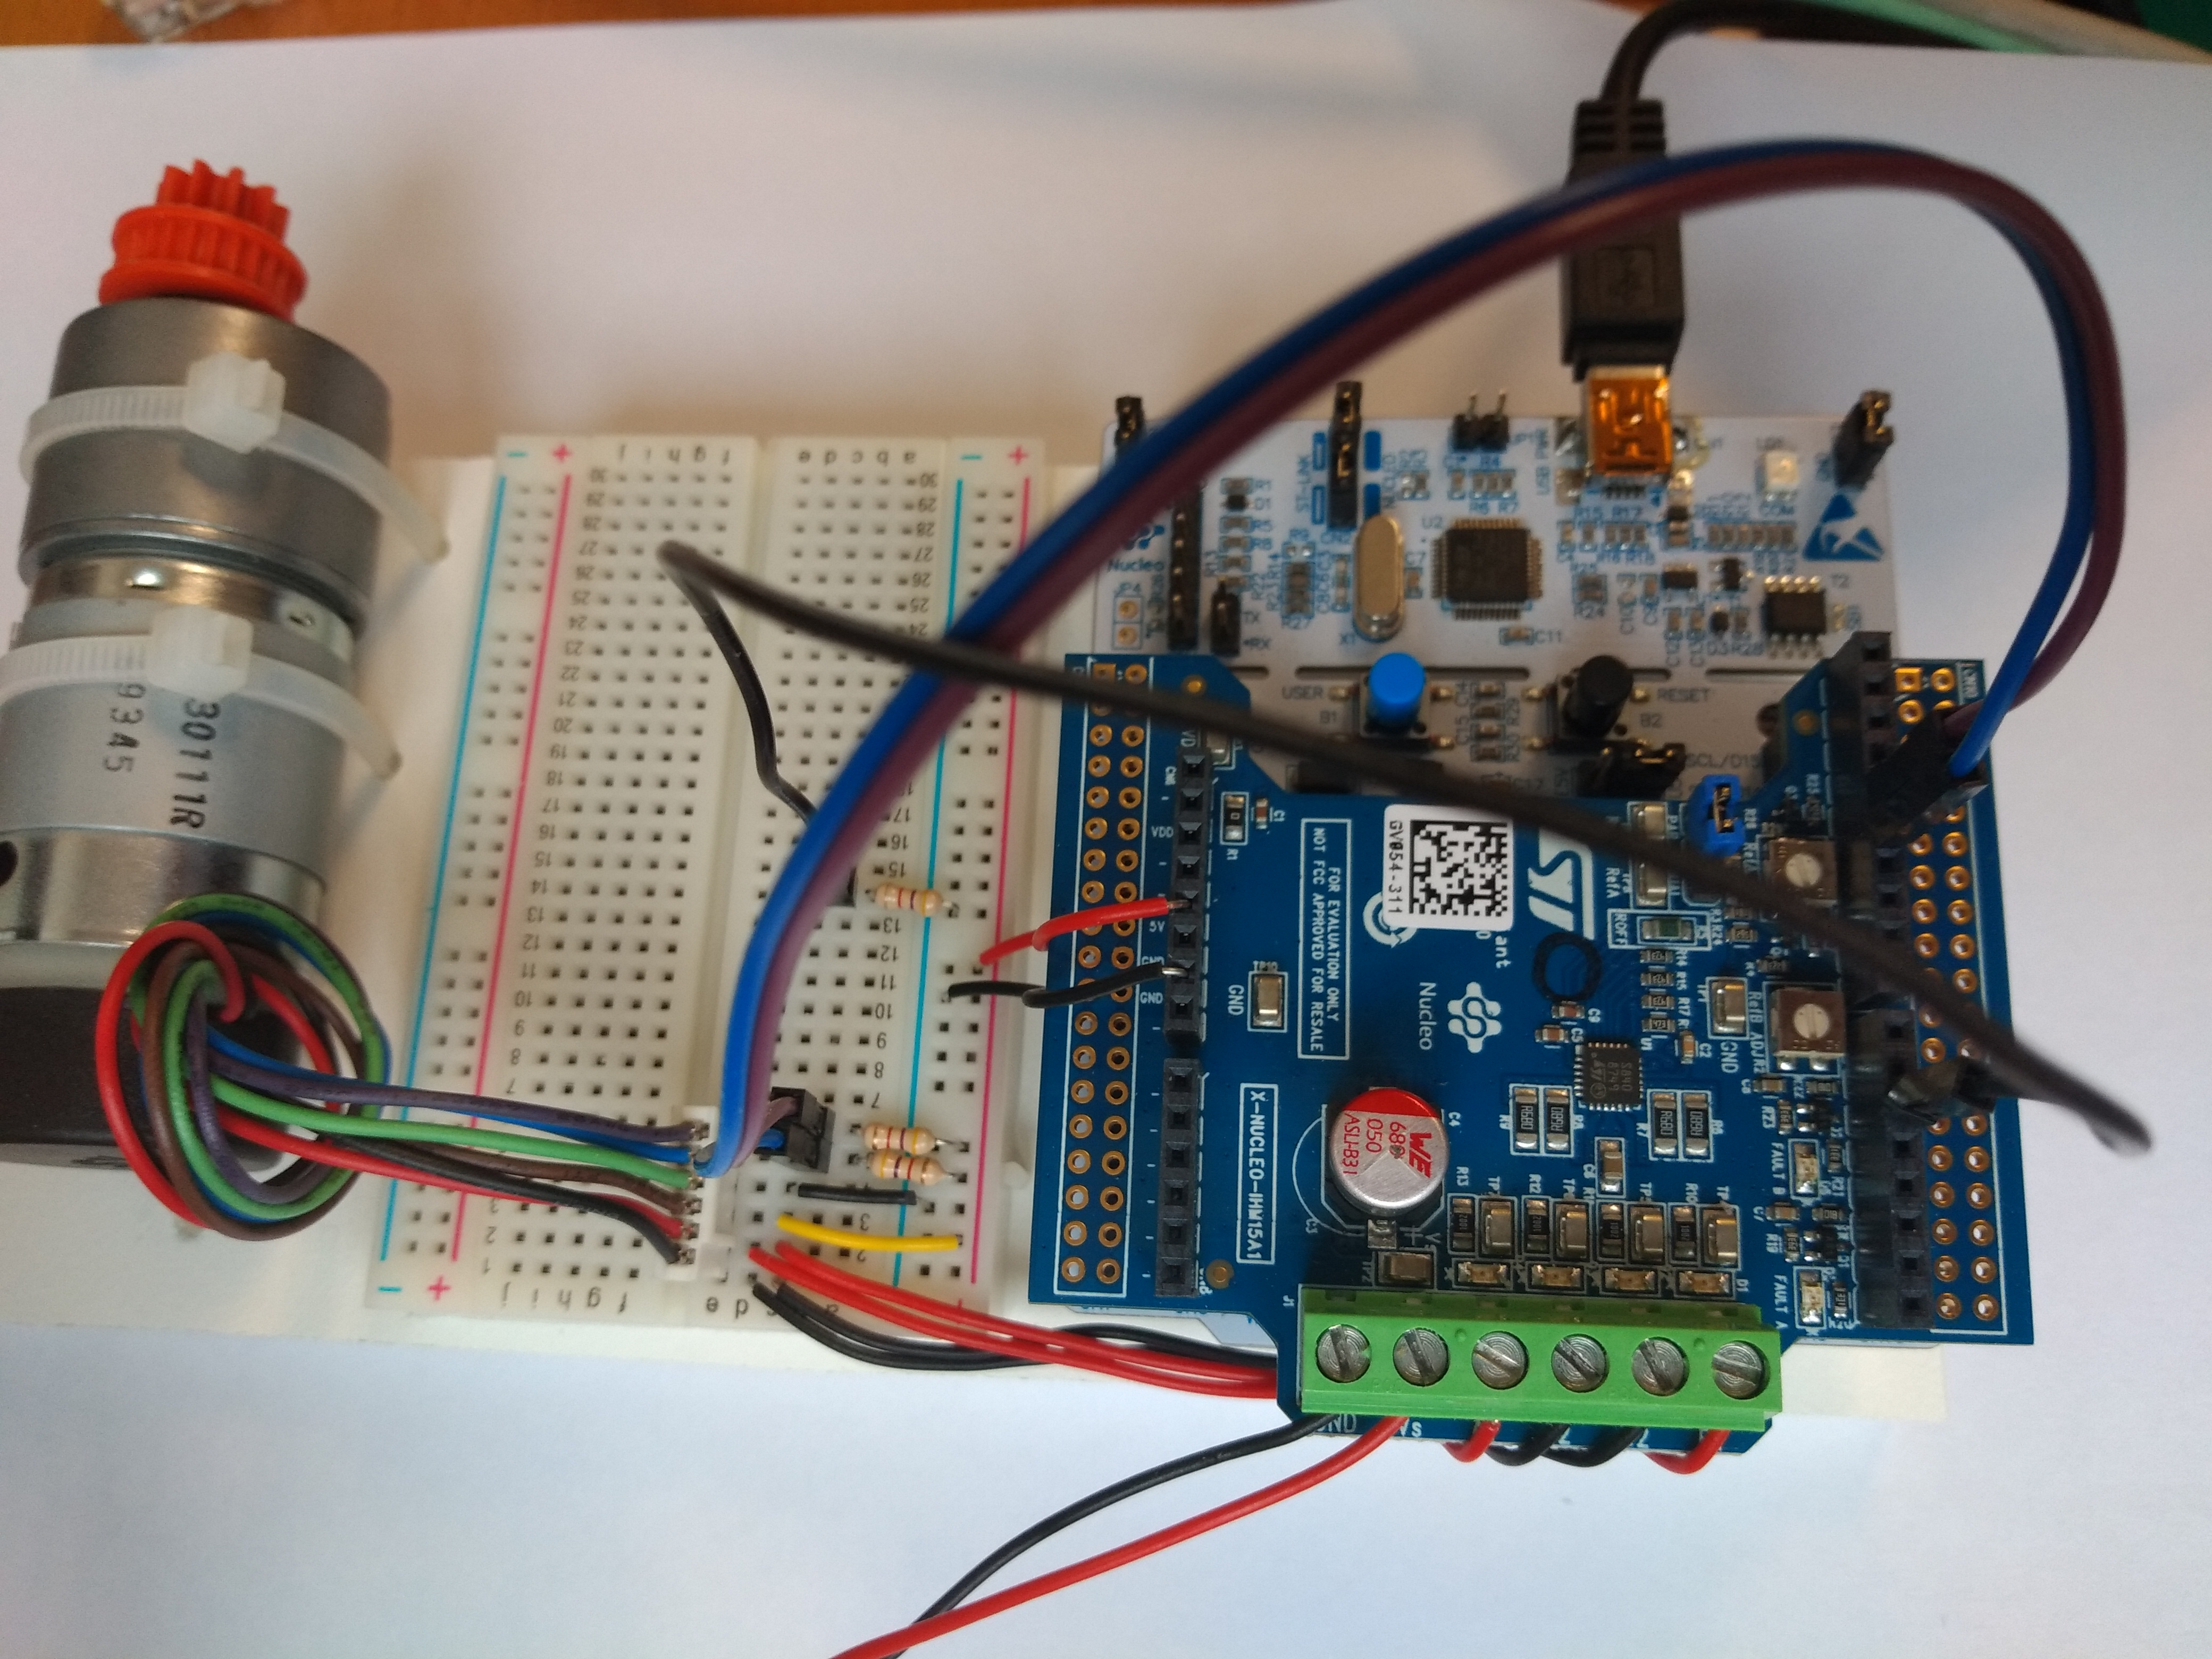
\includegraphics[scale=0.15,angle=90]{montaje2.jpg}
\caption{vista del montaje completo}\label{f14}
\end{figure}
\chapter{Descripción del \emph{software} del sistema \protect \footnote{La descripción de software corresponde a la versión de Matlab R2021b.}}
\section{Uso de Matlab/Simulink para la generación de Código}
En esta sección describiremos el software que vamos a emplear para el desarrollo de  las prácticas. El procesador empleado por la placa de desarrollo es un ARM. El fabricante suministra diversos entornos de desarrollo y \emph{tool-chains} para elaborar programas en lenguaje C/C++, compilarlos y descargar el ejecutable obtenido en la placa mediante el programador. También es posible programar y compilar a través de EMBED, un entorno de desarrollo disponible a través de la red. Una introducción a las distintas posibilidades de programación se puede encontrar en \cite{STNUCLEOSF}.
Sin embargo, en las presentes prácticas, no programaremos directamente las placas de desarrollo; dejaremos que Matlab/Simulink lo haga por nosotros. En concreto, Simulink ofrece soporte para la programación de placas de la familia NUCLEO.  Dicho soporte ofrece la posibilidad de emplear bloques de Simulink para leer y escribir en los pines de la placa y ejecutar en la misma modelos desarrollados con bloques de Simulink. Además, permite mantener una conexión a través de un puerto serie entre la placa y Simulink, de modo que es posible leer y representar gráficamente variables generadas en la placa, empleando las herramientas estándar de Simulink.

Veamos en primer lugar cómo preparar Simulink para trabajar con una placa NUCLEO.
\subsection{Configuración de Matlab/Simulink}
\paragraph{Descarga e instalación del software para Simulink} En primer lugar, es preciso instalar un \emph{Add-on} para incorporar el \emph{software} necesario. Para ello, abrimos una sesión de Matlab y nos conectamos desde la ventana de Matlab a nuestra cuenta de Mathworks. A continuación, pulsamos el botón \emph{Add-ons}. La figura \ref{f15} muestra una captura de pantalla donde se han señalado con un círculo rojo tanto el lugar donde abrir sesión como el botón \emph{Add-ons}.
\begin{figure}
\centering
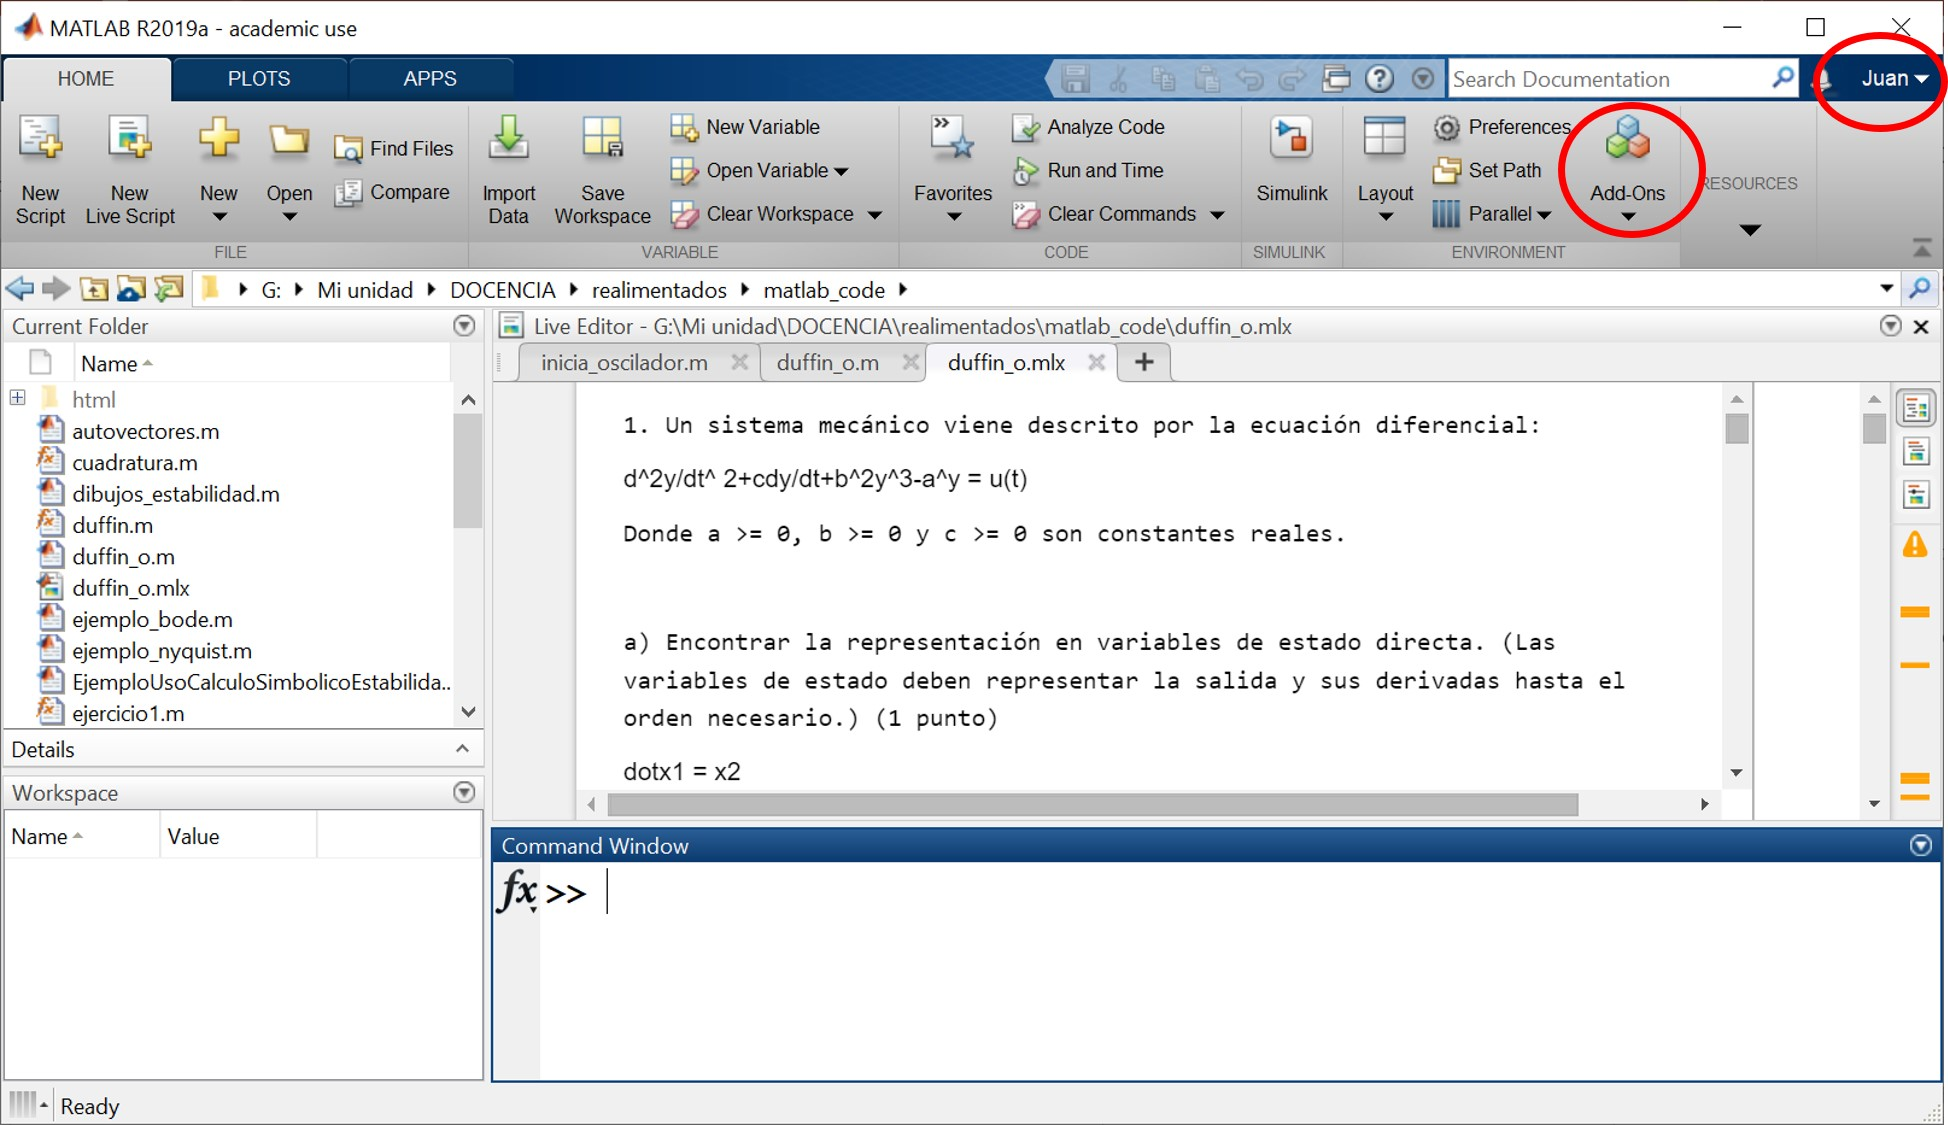
\includegraphics[scale=0.5]{matlab.jpg}
\caption{Ventana de Matlab con el botón \emph{Add-ons} señalado en rojo}\label{f15}
\end{figure}
Al pulsar el botón \emph{add-ons} se nos abre un navegador con todos los módulos disponibles. Para encontrar el que necesitamos basta poner en el campo de búsqueda \emph{Nucleo} ó \emph{Nucleo board}. El navegador nos lleva hasta el sitio de descarga e instalación del módulo para programar placas de la familia Nucleo. A continuación es suficiente con seguir las instrucciones para descargar e instalar el software. Básicamente, Matlab nos instalará una nueva librería de Simulink, con bloque específicos para manejar los pines de la placa (entradas/salidas digitales), generar señales de PWM o configurar y manejar distintos protocolos de comunicaciones. La figura \ref{f16} muestra una vista de la librería. 

\begin{figure}
\centering
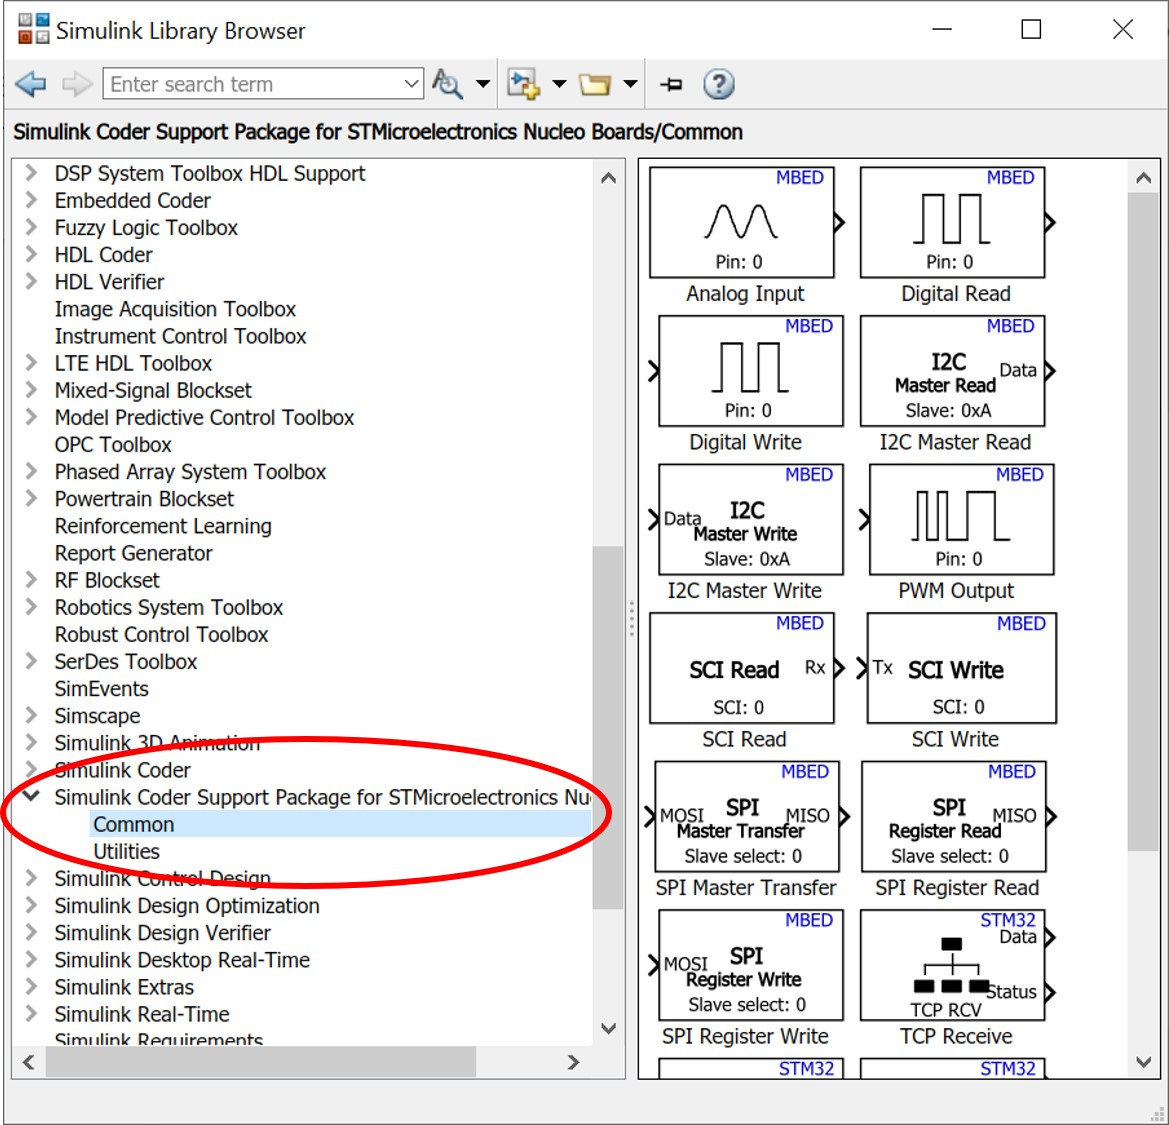
\includegraphics[scale=0.5]{sbroser.jpg}
\caption{Librería de Simulink para las placas ST Nucleo}\label{f16}
\end{figure} 

Además de la nueva librería para Simulink, también se instala el software necesario para generar código C/C++ a partir de los modelos que creemos en Simulink  y un compilador cruzado para compilar el código generado para que pueda emplearse en la placa. No examinaremos en detalle el funcionamiento de estos elementos. Los interesados pueden encontrar toda la información necesaria en la documentación \emph{on-line} de Matlab \cite{slkhelp}.

Se pueden construir modelos en Simulink, combinando los bloques de la librería específica para las placas Nucleo con el resto de bloques de Simulink. Dependiendo de la configuración que se dé al modelo de Simulink construido pueden suceder varias cosas:
\begin{itemize}
\item El Modelo desarrollado se ejecuta en modo \emph{run onboard/external}. En dicho caso cuando se ejecuta el modelo de Simulink, este convierte todo el modelo en código C/C++, lo compila para la placa y lo descarga en la misma empleando la conexión USB del programador de la placa. Simulink tan solo se encargaría de recibir datos y enviar órdenes a través de la conexión USB que, en este caso, emula un puerto serie. También ejecutaría el código necesario para visualizar variables.  Éste será el modo que emplearemos en estas prácticas.

\item El modelo desarrollado se ejecuta en modo \emph{PIL (Procesor In the Loop)}. En este modo, parte del código se ejecuta en Simulink y parte en la placa, intercambiando ambos sistemas información a través de la conexión USB. 
 
\end{itemize}
\paragraph{Instalación del driver ST-Link/V2 USB}
Como se ha indicado antes, para intercambiar datos entre Simulink  y la placa de desarrollo se emplea la conexión USB, sobre la que se emula un puerto serie. Para que funcione correctamente es preciso instalar un \emph{driver} específico suministrado por STMicroelectronics. El \emph{driver} puede descargarse de la página web: \url{https://www.st.com/en/development-tools/stsw-link009.html}.
\paragraph{Ejemplo de configuración}
Una vez que todo está instalado correctamente, vamos a ver mediante un ejemplo sencillo como crear y configurar un modelo de Simulink. 
Una primera cuestion \emph{MUY IMPORTANTE}: la programación de la placa de control emplea un fichero MAKEFILE para compilar-enlazar-descargar el software. Dicho fichero da problemas si la ruta del archivo de simulink de nuestro modelo tiene nombres con caracteres especiales o con espacio. Para asegurar que el proceso de compilación funcione correctamente lo mejor es crearse un fichero de trabajo directamente en C:/ y darle un nonbre sencillo: C:/practica. (no acentos, no espacios \sout{C:/Mis prácticas})
La figura \ref{f17} muestra los pasos a seguir. En nuestro caso, vamos a crear un modelo que permite mediante un botón deslizable encender y apagar un led de la placa. Para ello hemos seleccionado y conectado los siguientes bloques; (ver figura \ref{f17a}):
\begin{itemize}
\item Simulink/Sources: Un bloque con una entrada constante.
\item Simulink/Dashboard: Un bloque Slider Switch
\item Simulink Coder Support Package for STmicroelectronics Nucleo Boards/Common: Un bloque Digital Write  
\end{itemize}
El interruptor deslizable está conectado al bloque de entrada constante de modo que cambia su valor entre cero y uno. El valor del bloque es enviado al pin que configuremos en el bloque Digital Write. Si consultamos el mapa de pines de la placa (figura \ref{f12}) comprobamos que el led1 está conectado al pin D13. Por tanto configuramos la dirección del bloque Digital Write a dicha dirección (basta hacer doble \emph{clik} en el bloque y escribir la dirección). Una vez completado el modelo, necesitamos configurarlo para que Simulink genere el código y lo descargue en la placa.


En primer lugar conectamos la placa a un puerto USB del ordenador. A continuación en la ventana de Simulink donde hemos construido el modelo, seleccionamos, en la parte superior la ventana la pestaña MODELLING, Esto modifica las opciones de la ventana de configuración de parámetros que, abrimos a continuación pulsando el botón \emph{settings}. En el menú desplegable que aparece pulsamos la opción Model Properties (figura \ref{f17b}).  

Se abre una nueva ventana que nos permite configurar los parámetros del modelos.  Seleccionamos la opción \emph{Hardware implementation} y elegimos de entre las opciones disponibles la que corresponde a nuestra placa: ST32 Nucleo F411RE (figura \ref{f17c}). 

Una vez selecionada, y dentro todavía de la opción \emph{Hardware implementation}, desplegamos la pestaña \emph{Target Hardware Resources} y seleccionamos la opción \emph{External mode} (figura \ref{f17d}). Nos aparecerá una ventana en la que se nos indica que la conexión entre ordenador y placa se realizará a través de un puerto serie (emulado sobre el puesto USB). Debemos escribir la dirección de dicho puerto en la entrada marcada como \emph{Serial port}. En la figura \ref{f17e} se ha introducido el puerto \textbf{COM4}. 

Hay que comprobar en cada caso qué puerto serie ha asignado el ordenador a la placa cuando se conectó al ordenador. Para hacerlo hay que ir a los parámetros de configuración del ordenador y buscar en \emph{Configuración de dispositivos e impresoras} el \emph{driver} de la placa: STM32 STLink (figura \ref{f17g}). Dentro de la propiedades del \emph{driver}, en la pestaña \emph{Hardware}, encontramos el puerto COM asignado al \emph{driver} (figura \ref{f17h}).

Una vez acabado este proceso, y tras salvar los cambios, Volvemos a la ventana del modelo. Si se han realizado los pasos anteriores correctamente, se habrá creado en la ventana del modelo una nueva pestaña con la etiqueta HARDWARE. Esta es la pestaña en la que trabajaremos siempre que usemos la placa (figura \ref{f17f}). 

\begin{figure}
\begin{subfigure}{0.5\textwidth}
\centering
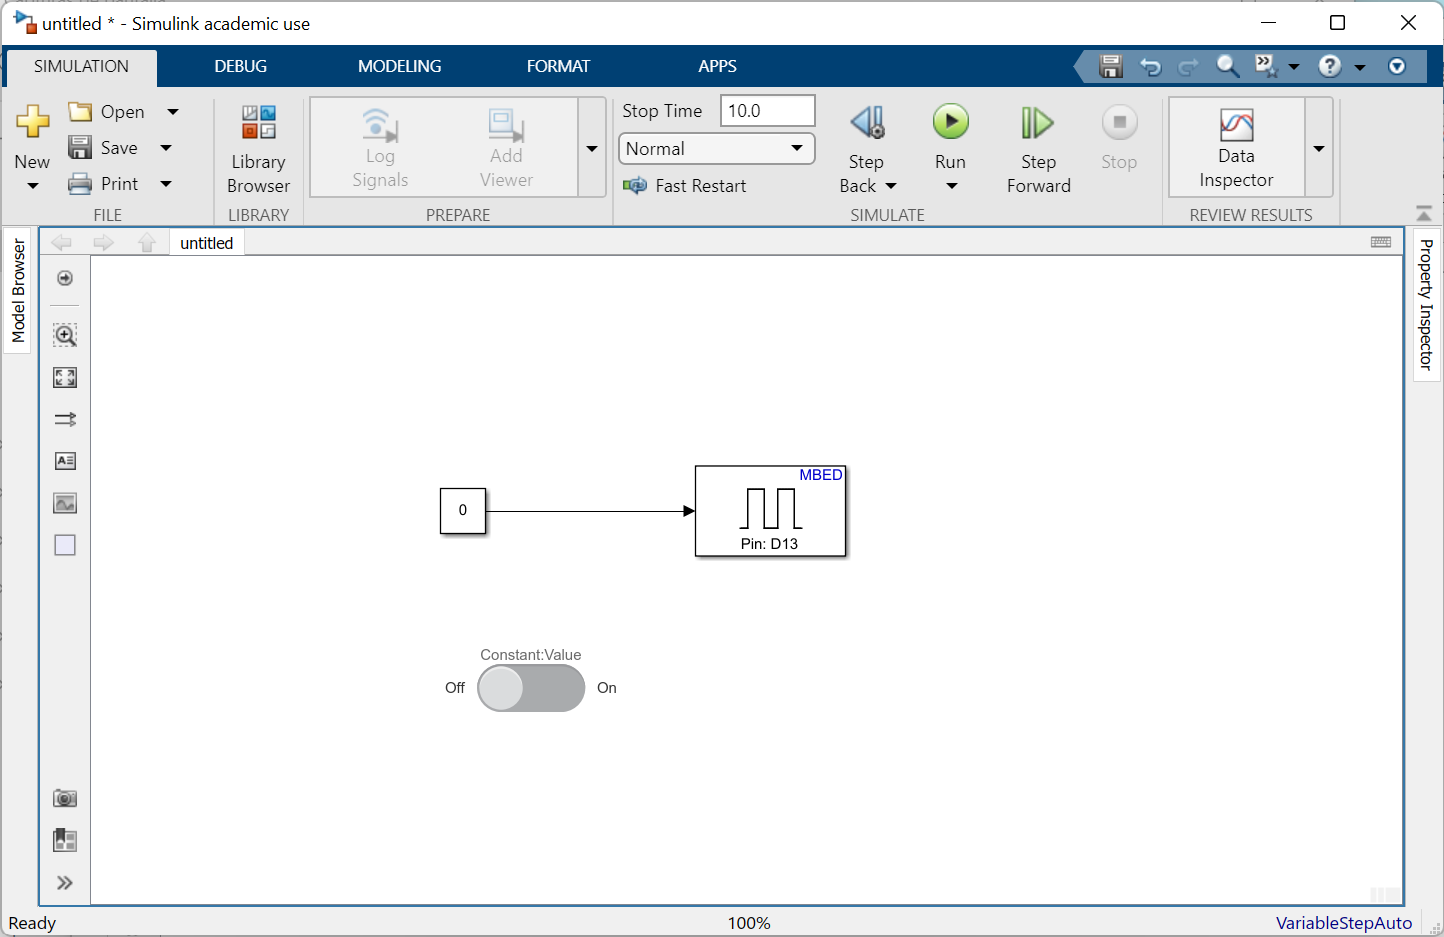
\includegraphics[width = \linewidth]{ejemplo1.png}
\caption{Modelo}\label{f17a}
\end{subfigure}
\begin{subfigure}{0.5\textwidth}
\centering
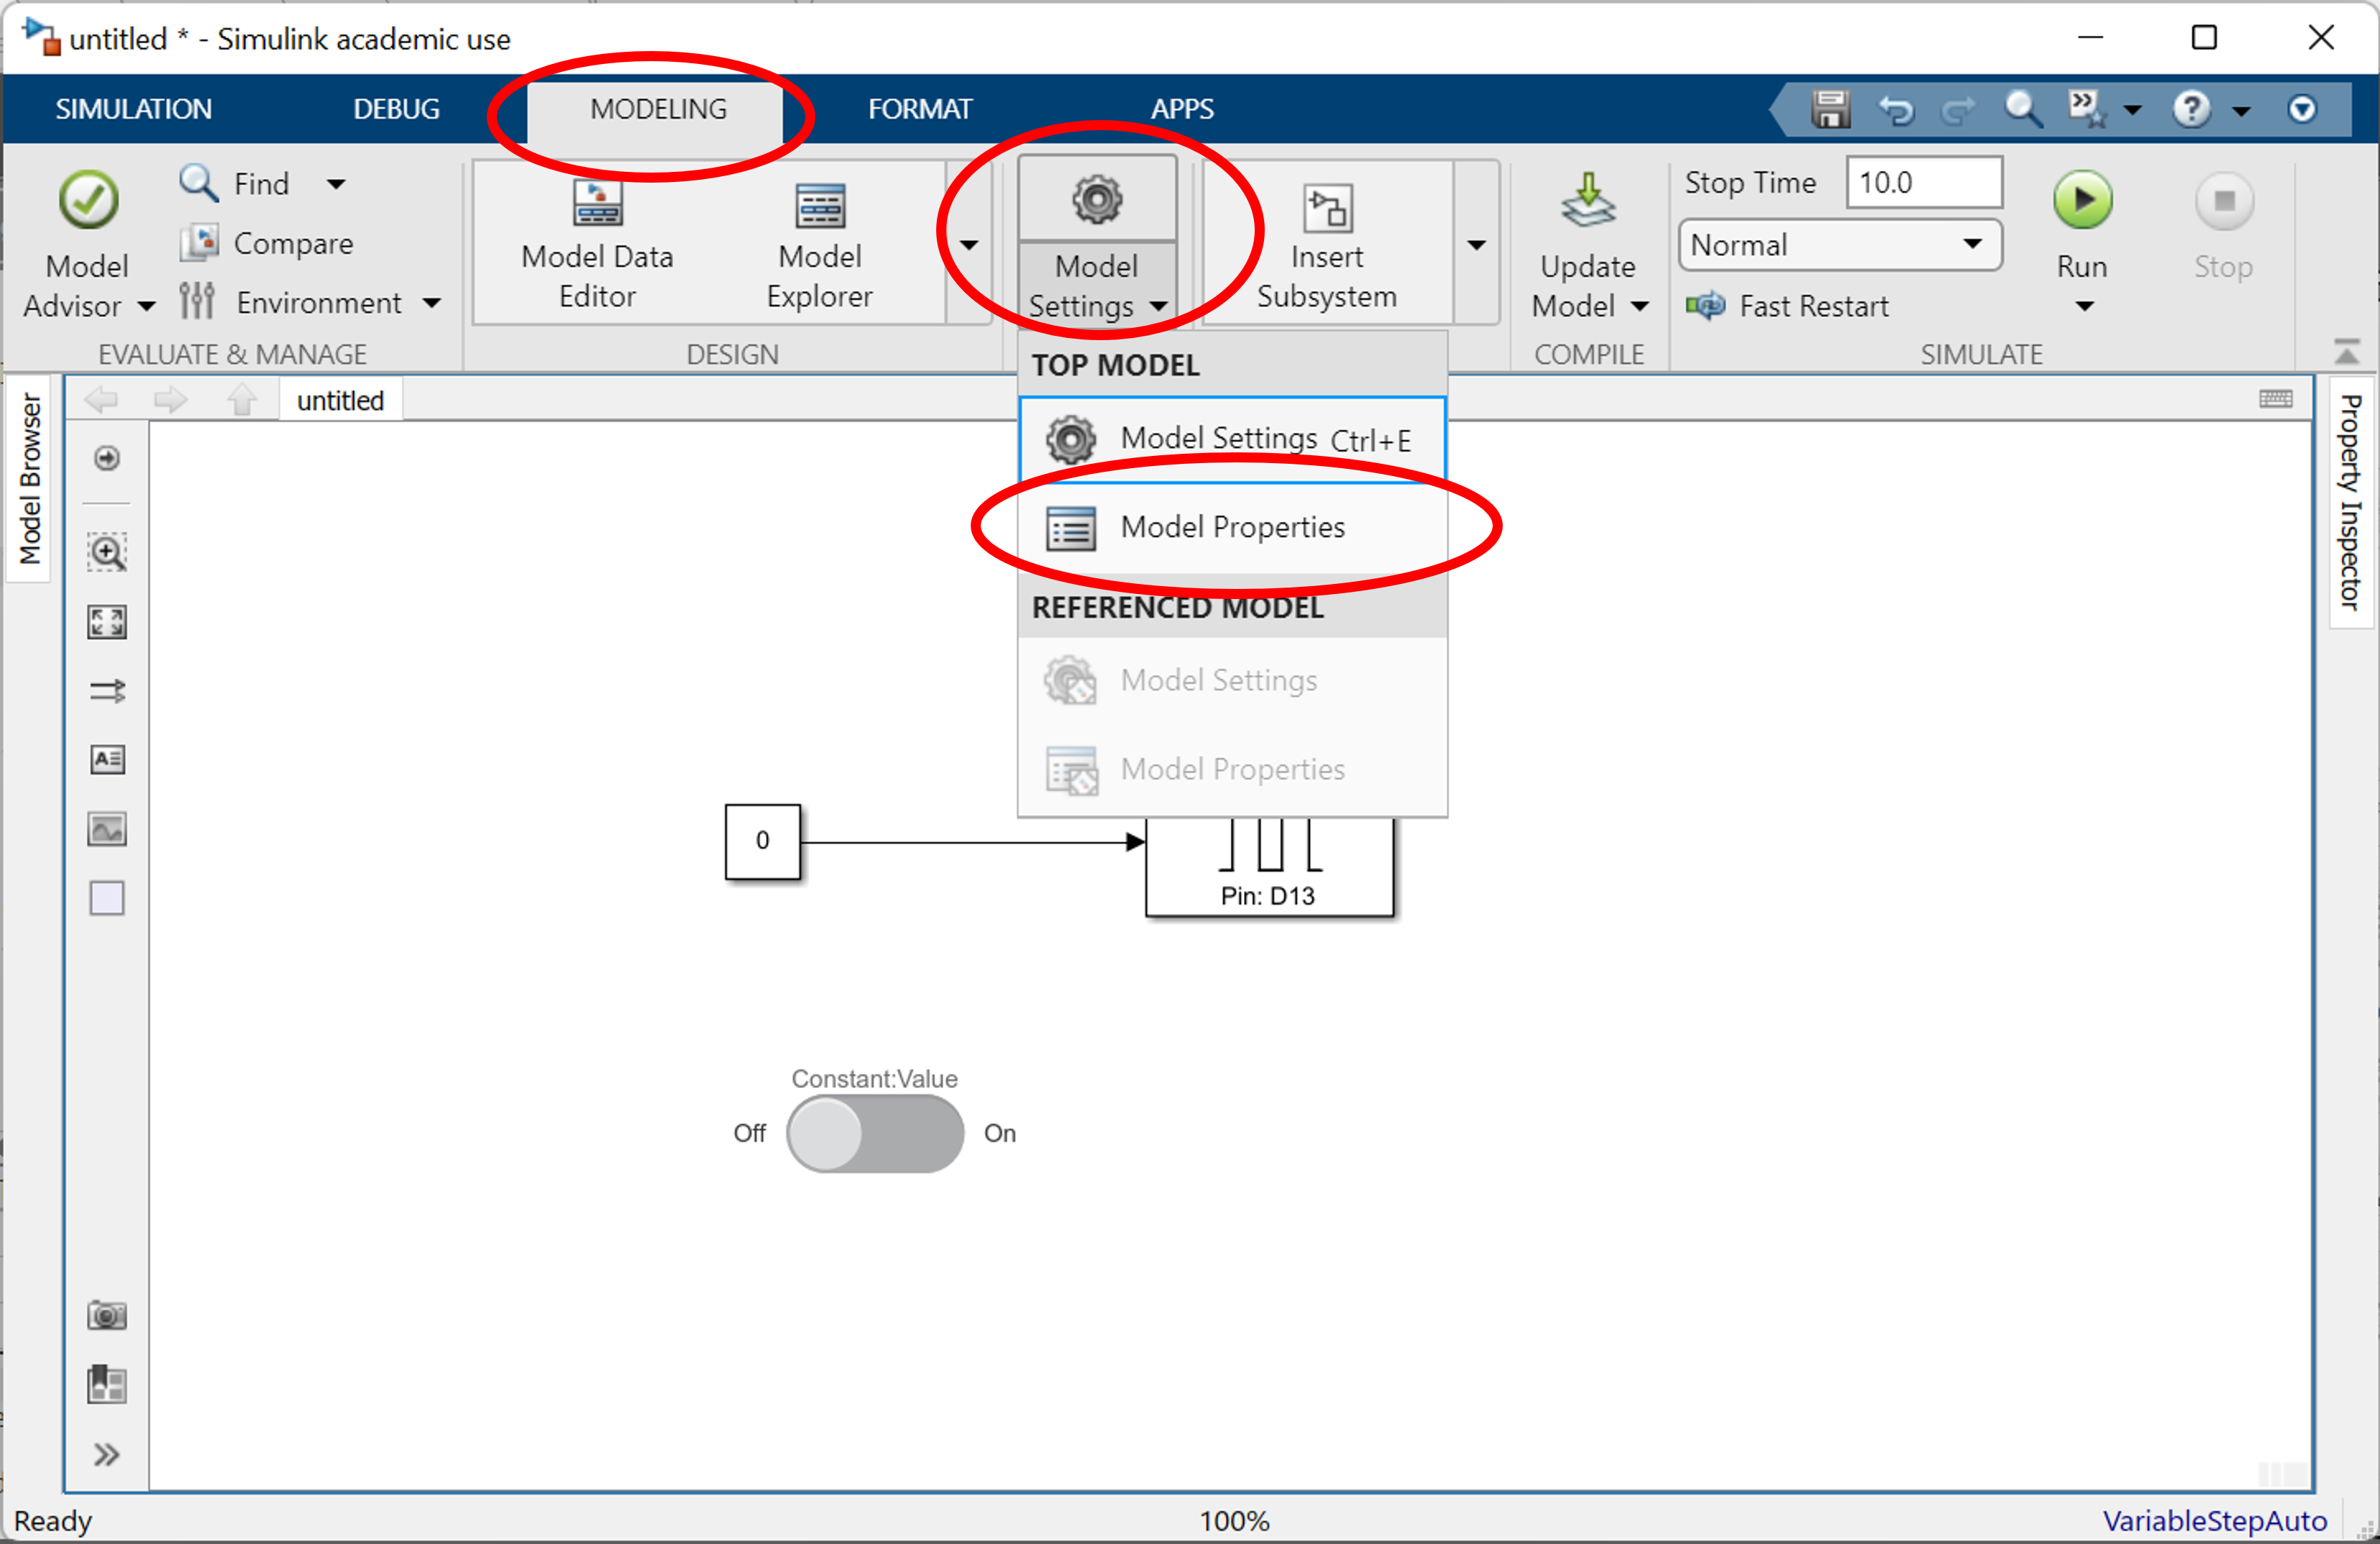
\includegraphics[width = \linewidth]{settings1.png}
\caption{Acceso a la ventana de configuración}\label{f17b}
\end{subfigure}
\begin{subfigure}{0.5\textwidth}
\centering
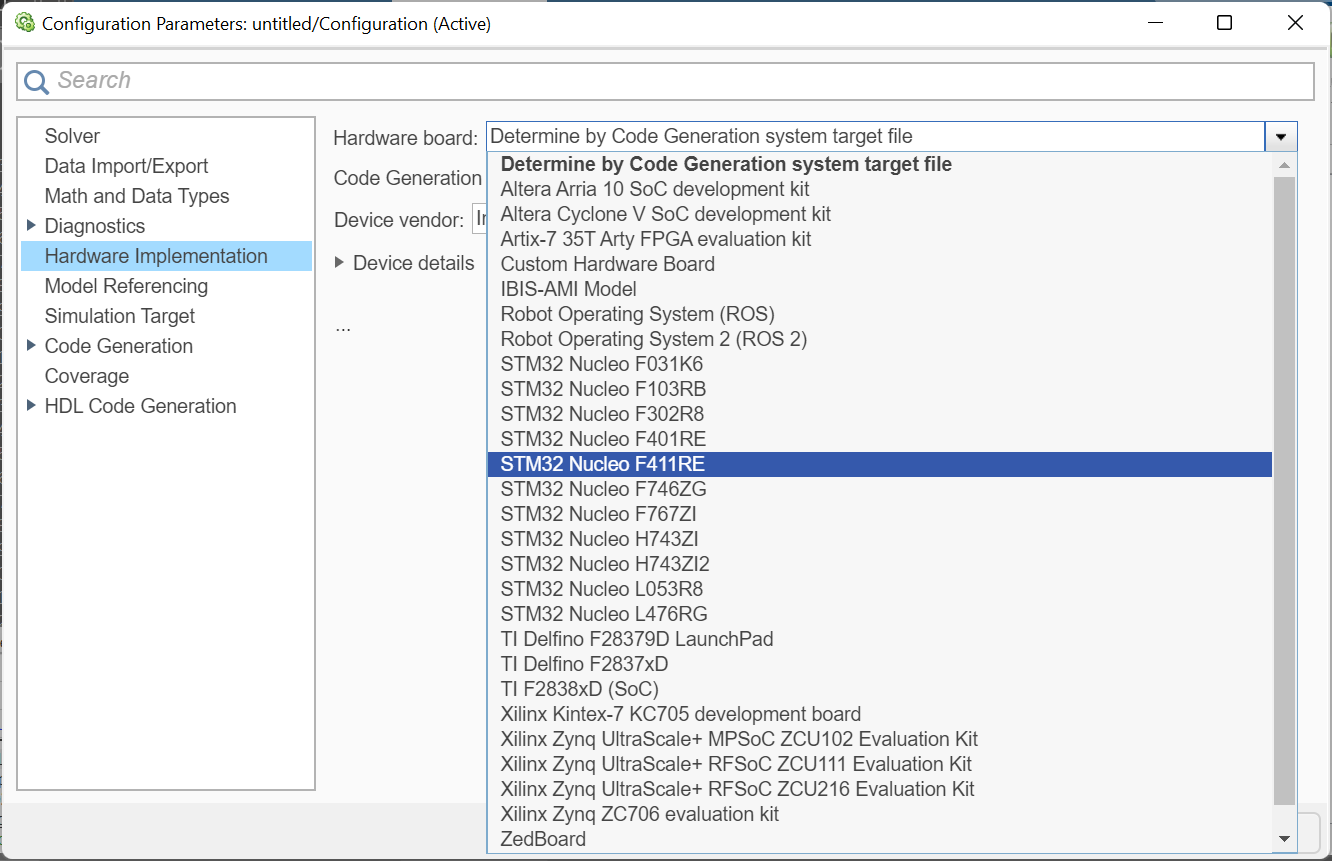
\includegraphics[width = \linewidth]{settings2.png}
\caption{Selección de la placa}\label{f17c}
\end{subfigure}
\begin{subfigure}{0.5\textwidth}
\centering
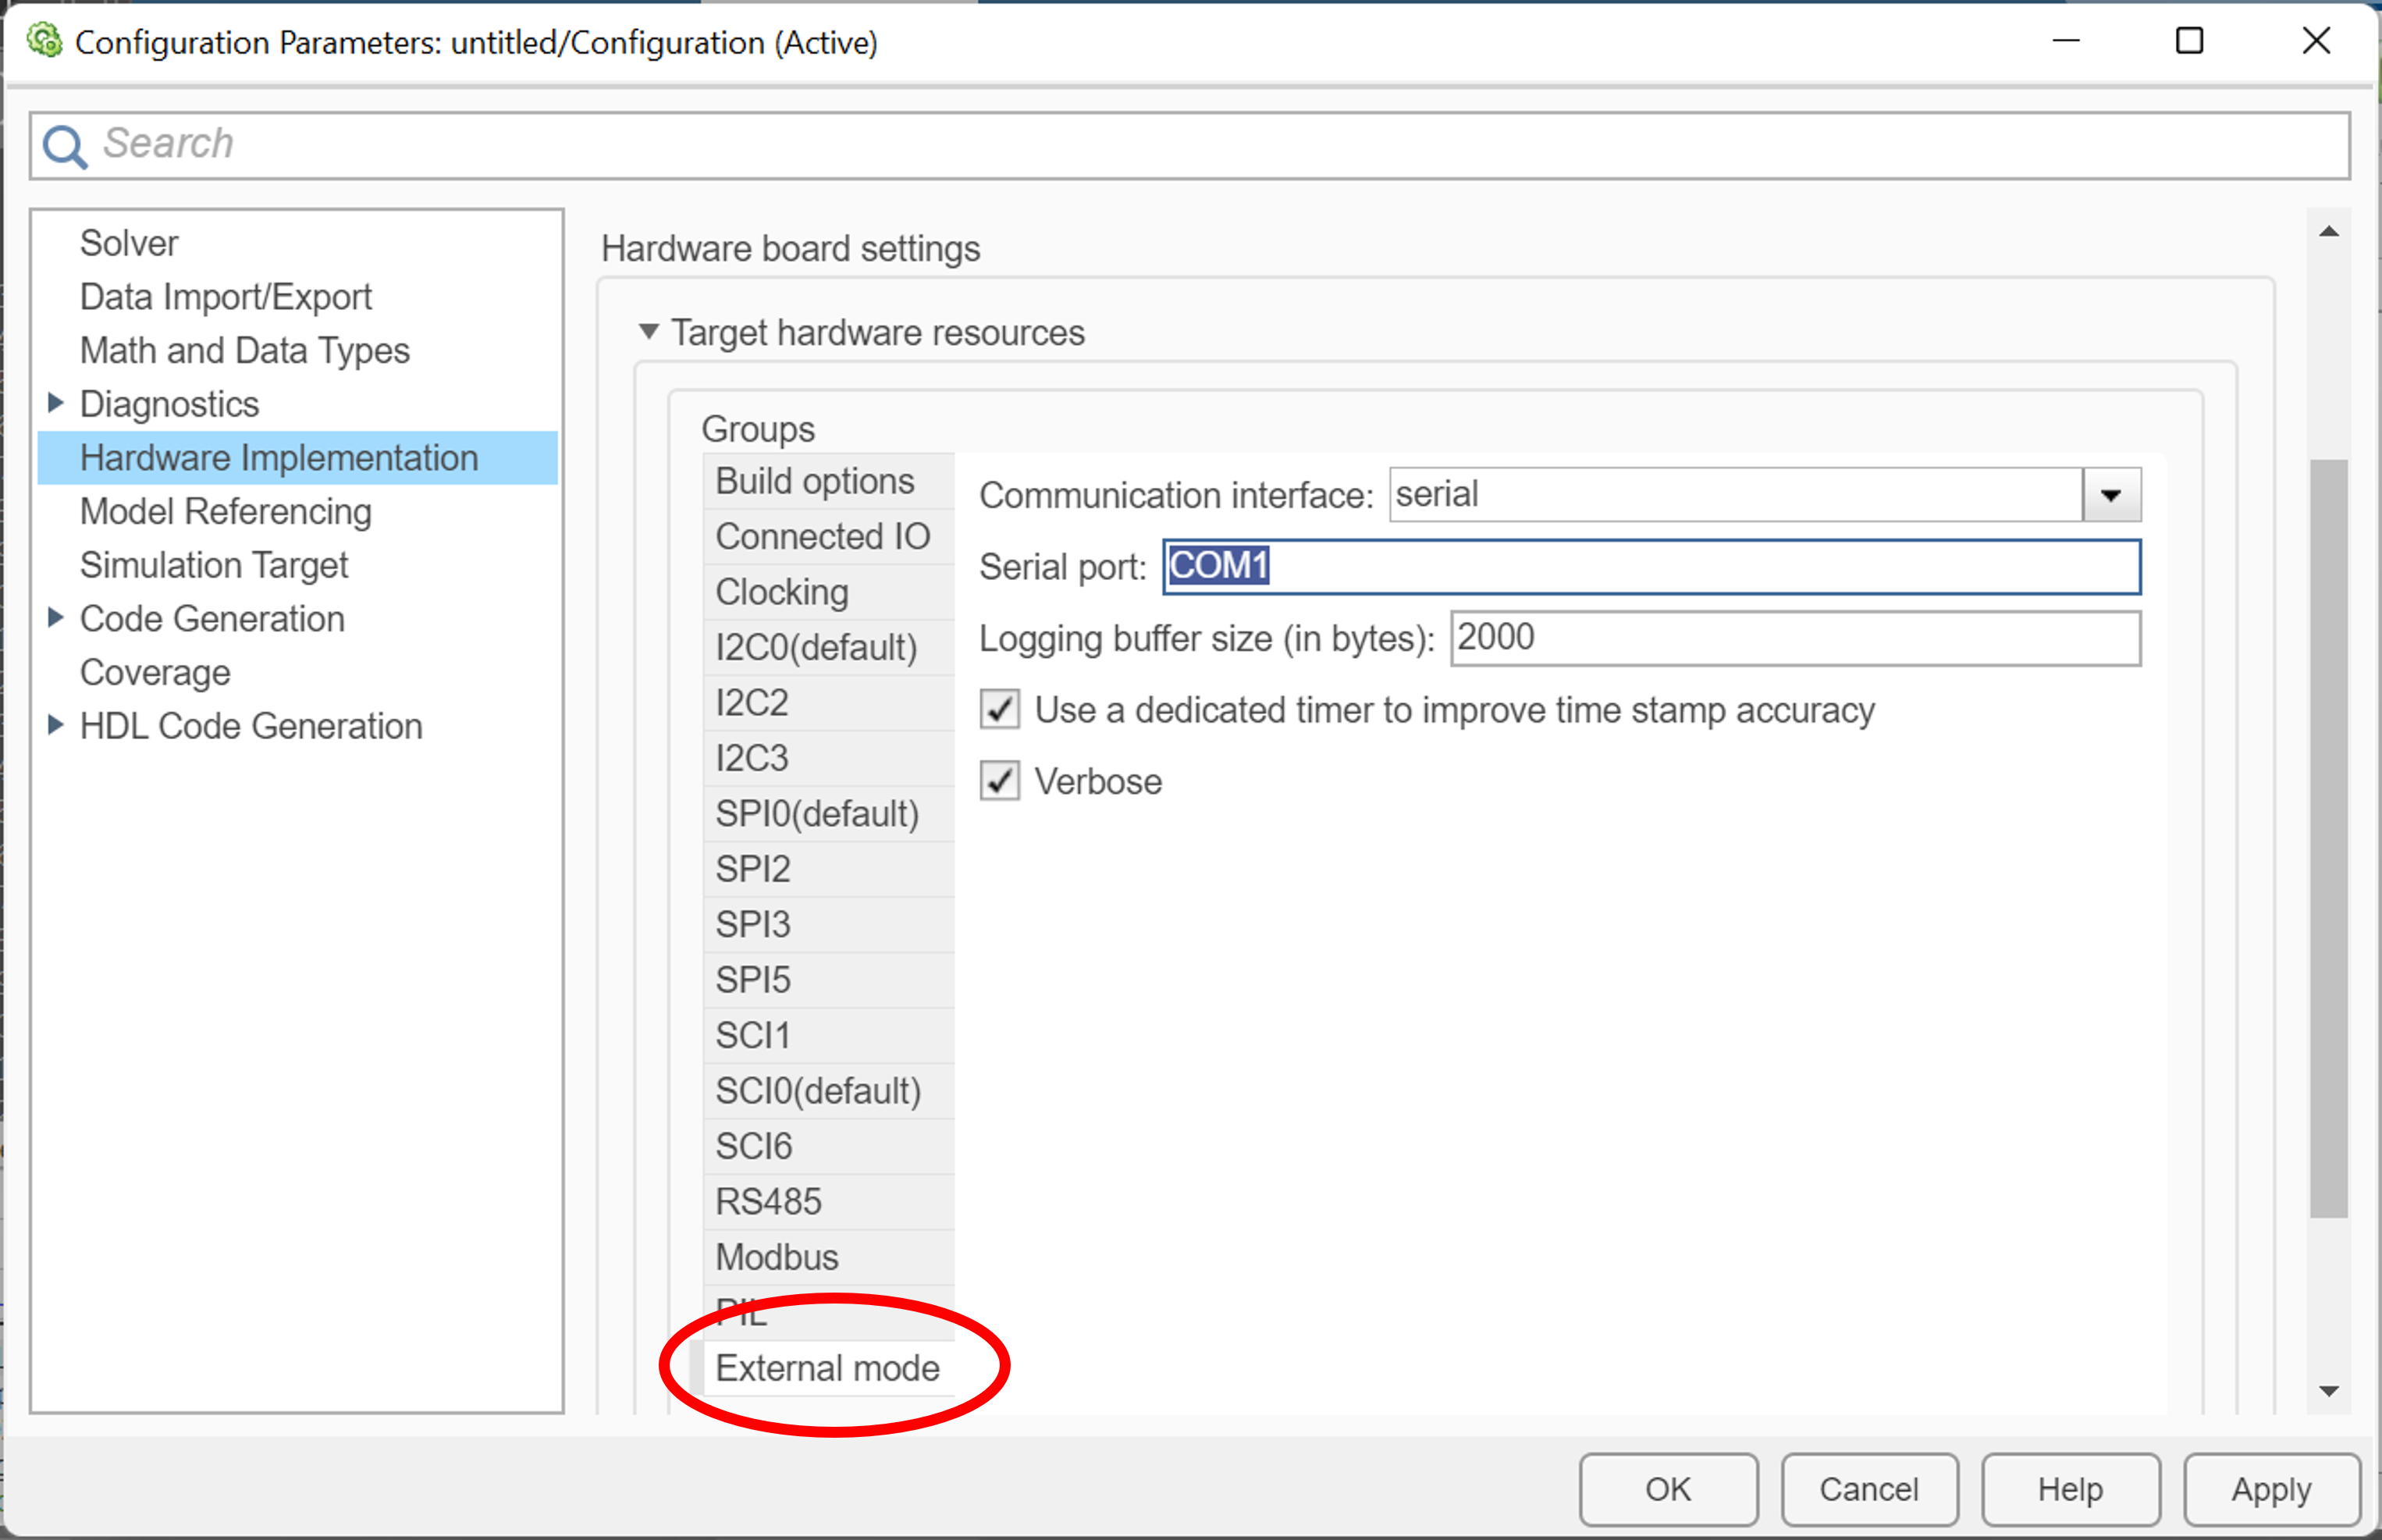
\includegraphics[width = \linewidth]{settings3.png}
\caption{Acceso a parámetros de External Mode}\label{f17d}
\end{subfigure}
\begin{subfigure}{0.5\textwidth}
\centering
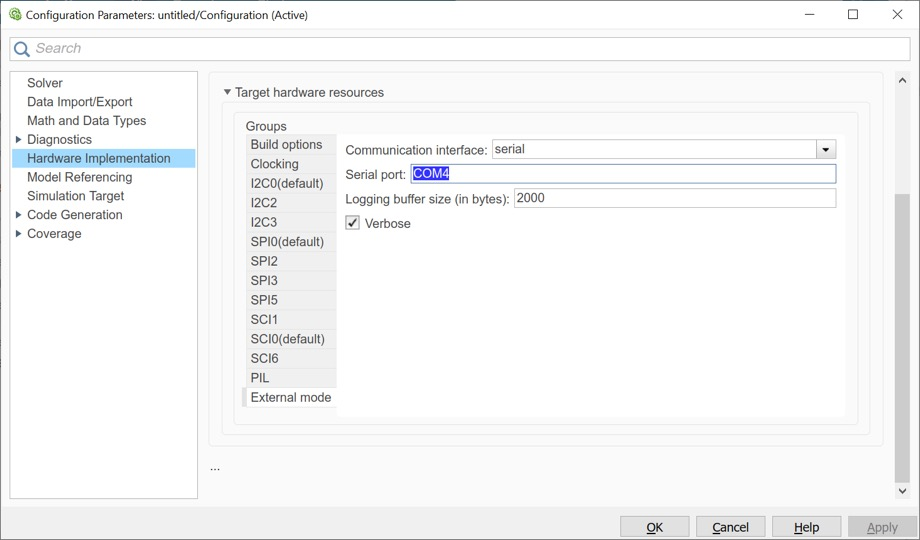
\includegraphics[width = \linewidth]{eje6.jpg}
\caption{Ajuste del valor de puerto serie (COM) asignado al Driver}\label{f17e}
\end{subfigure}
\begin{subfigure}{0.5\textwidth}
\centering
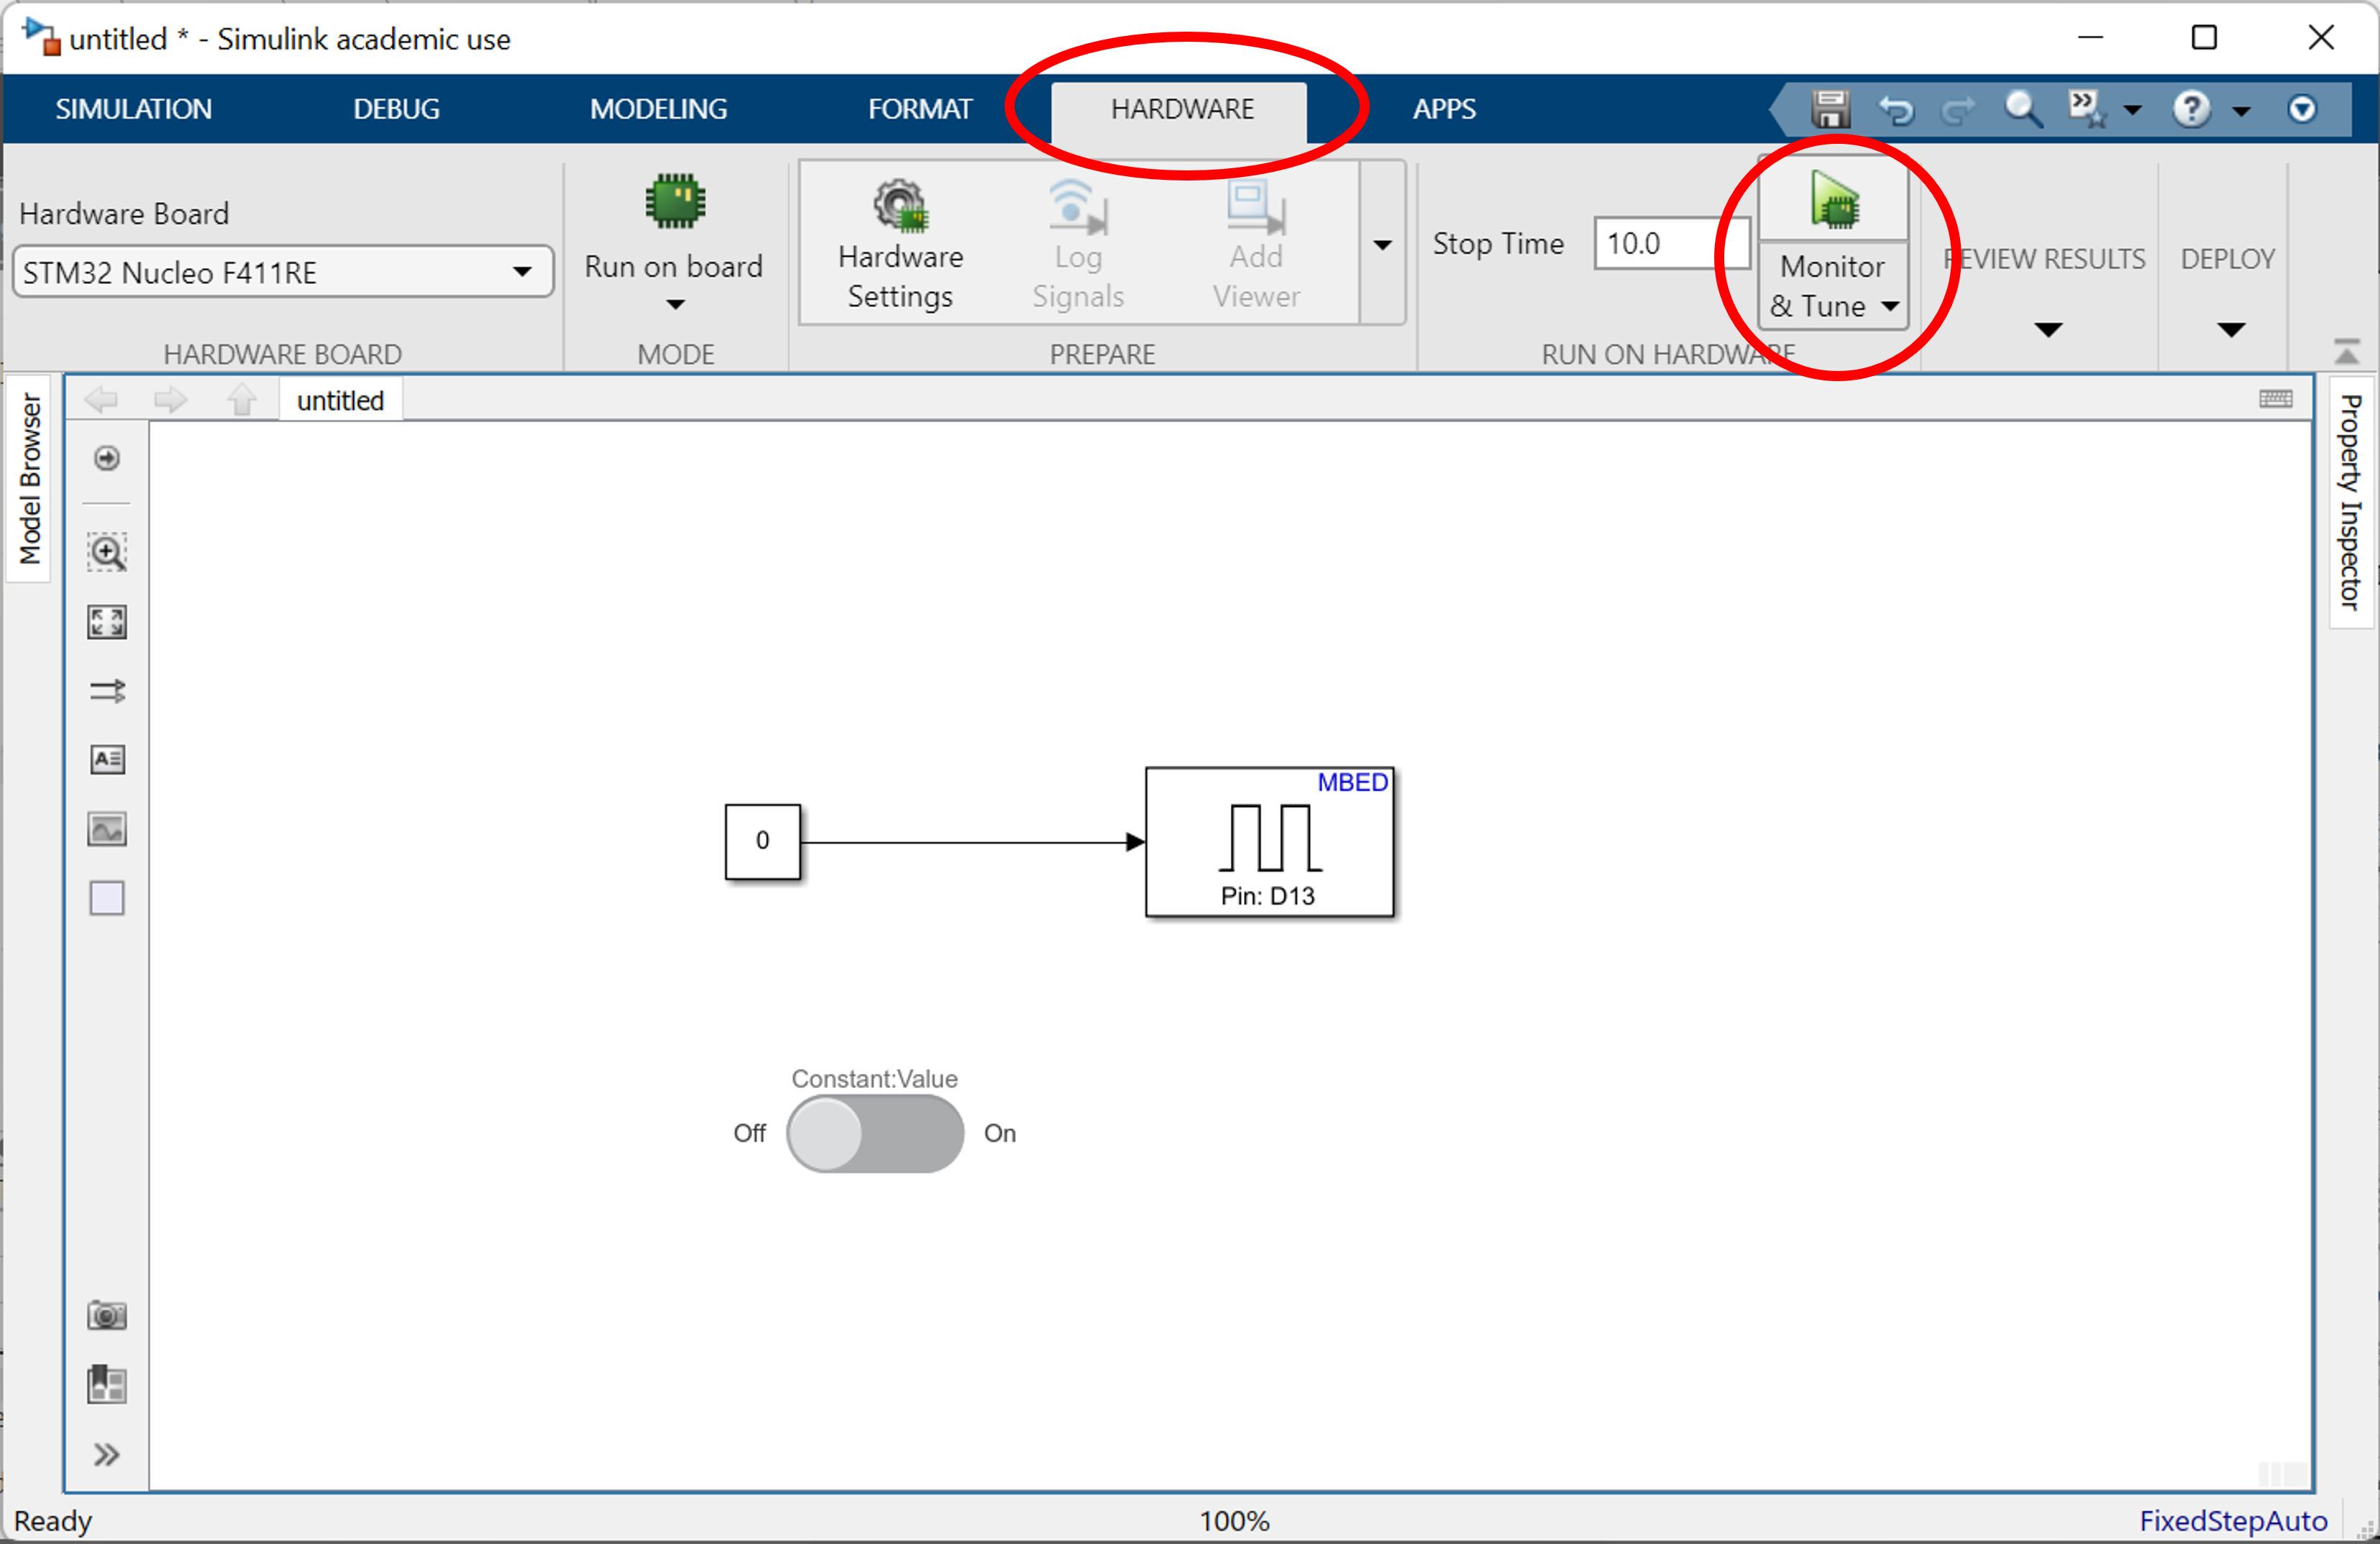
\includegraphics[width = \linewidth]{settings4.png}
\caption{Pestaña HARDWARE de la ventana del modelo}\label{f17f}
\end{subfigure}
\begin{subfigure}{0.5\textwidth}
\centering
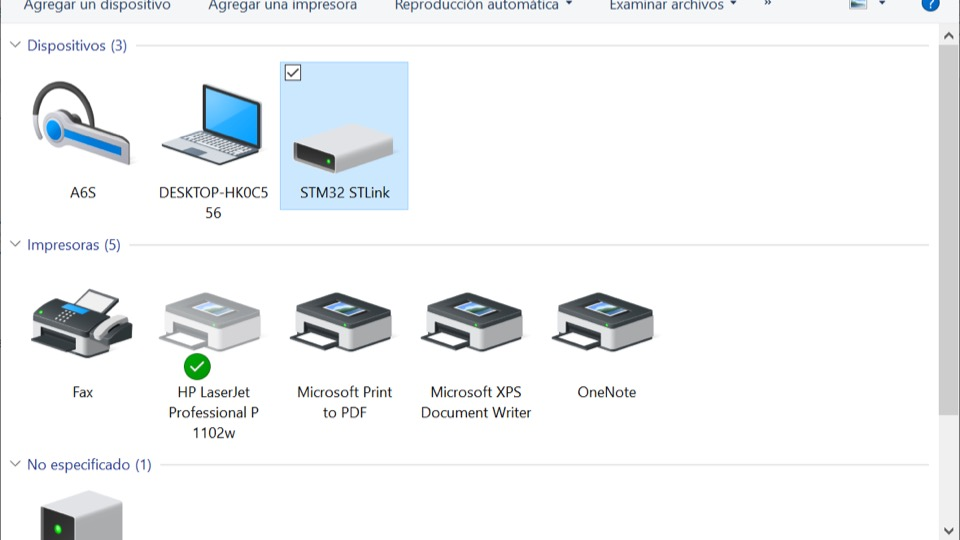
\includegraphics[width = \linewidth]{eje7.jpg}
\caption{Dispositivos. Driver: STM32 STLInk}\label{f17g}
\end{subfigure}
\begin{subfigure}{0.5\textwidth}
\centering
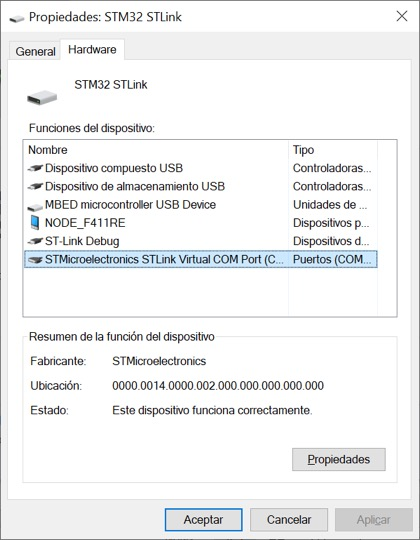
\includegraphics[width = 0.6\linewidth]{eje8.jpg}
\caption{Puerto COM asignado}\label{f17h}
\end{subfigure}

\caption{Ejemplo de modelo en Simulink para trabajar con la placa ST Nucleo}\label{f17}
\end{figure} 

\paragraph{Compilación, descarga y ejecución del modelo}
Una vez configurado el modelo, siguiendo los pasos del párrafo anterior, si pulsamos el botón \emph{Monitor \& Tune} del modelo, Simulink generará el código en C/C++ necesario, lo compilará, lo descargará en la placa y ejecutará el modelo durante el tiempo para el que se haya ajustado la duración del experimento.

El proceso de generación/compilación/descarga de código lleva un rato, por lo que hay que tener paciencia hasta que termine. Una vez terminado, Simulink genera una ventana de diagnóstico y lanza la ejecución. Si durante este tiempo cambiamos la posición del botón deslizante, veremos cómo encendemos y apagamos el led verde de la placa.

\chapter{Manejo del motor de continua en lazo abierto}
En esta primera práctica nos vamos a limitar a construir un modelo de Simulink que nos permita suministrar al motor un valor fijo de voltaje, y leer su posición y velocidad a través de los \emph{encoders}.
\section{Construcción del modelo}
\paragraph{Vista general del modelo} La figura \ref{f18} muestra una vista general del modelo; para facilitar su análisis se ha construido encapsulando sus bloques en distintos subsistemas.
\begin{figure}
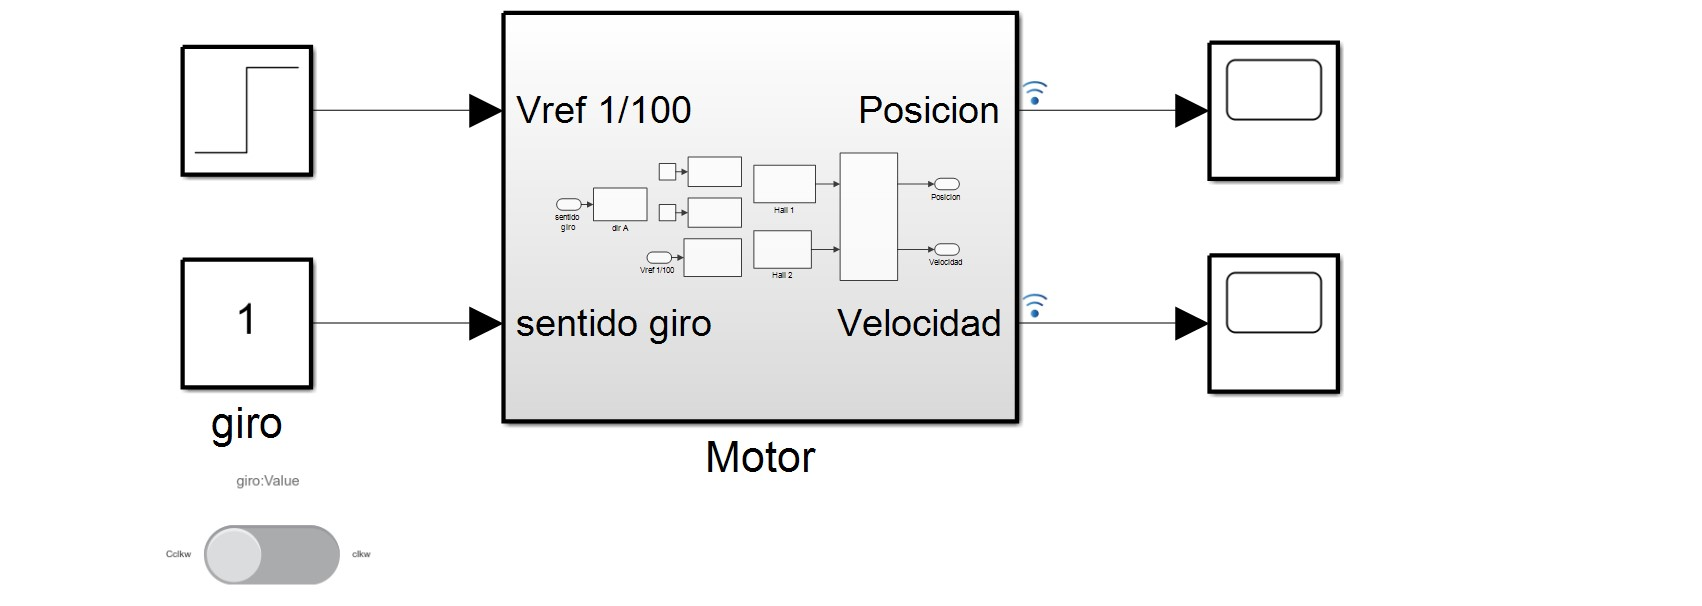
\includegraphics[width=\textwidth]{la1.jpg}
\caption{Esquema de Simulink para manejo del motor en lazo abierto. Vista general} \label{f18}
\end{figure}

En la figura se puede observar un bloque de entrada en escalón, que nos permitirá modificar el voltaje suministrado al motor y el instante de tiempo en que se suministra. Un bloque de entrada constante, cuyo valor podemos modificar mediante un botón deslizante (0 ó 1), su valor controlará el sentido de giro del motor.

El bloque central ---marcado como Motor--- contiene los bloque necesarios para interactuar con el motor. Lo veremos en detalle a continuación.

Las salidas del bloque Motor están conectadas a \emph{scopes} para poder observar la posición y la velocidad del motor. Es importante observar el símbolo que aparece encima de las líneas que unen el bloque con los \emph{scopes} Dicho símbolo  indica que se ha activado la recogida de los valores que toma dicha señal durante la ejecución del modelo. Ésto permite guardarlos, en archivos de datos, enviarlos al \emph{Workspace} de Matlab y, lo que es quizá más útil de todo, observarlos empleando el \emph{Simulation Data Inspector} (Ver ayuda de Simulink).
 
\paragraph{El bloque Motor}
si hacemos doble \emph{click} sobre el bloque Motor del modelo, accederemos a la estructura del subsistema que lo forma. La figura \ref{f19} muestra el contenido del bloque motor.
\begin{figure}
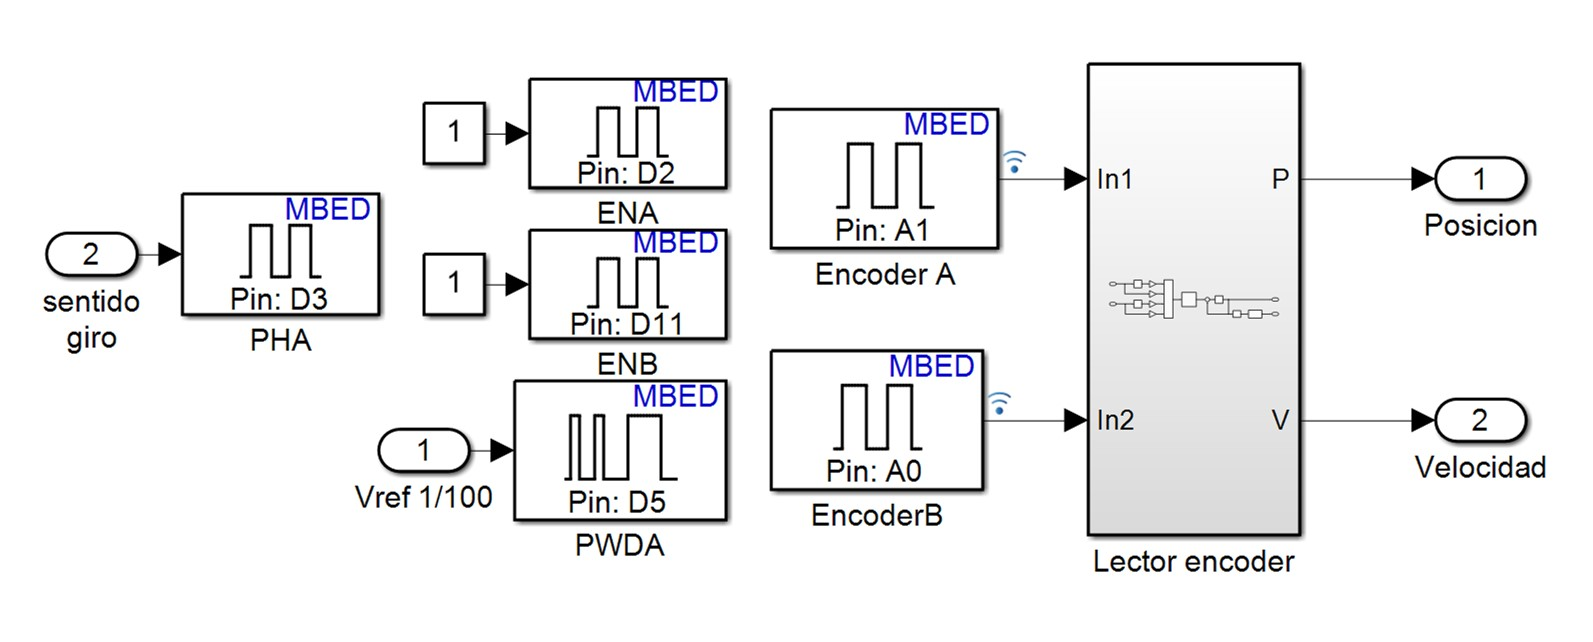
\includegraphics[width=\textwidth]{la2.jpg}
\caption{Estructura del bloque motor}\label{f19}
\end{figure}
Está compuesto por los siguientes bloques de Simulink:
\begin{itemize}
\item bloque PHA. Se trata de un bloque Digital Write de la librería Simulink Code support Package for STMicroelectronic Nucleo Boards. Recibe directamente el valor del bloque constante del modelo descrito anteriormente. Dicho valor se envía directamente al pin D3, dicho pin corresponde a la entrada PHA del la placa de expansión que controla el motor y que se encarga de cambiar el sentido de giro del motor (ver tabla \ref{t2} y figura \ref{f10}). Nos permite por tanto controlar manualmente el sentido de giro del motor.
\item Bloque ENA. Idéntico al anterior. Se ha puesto a un valor fijo 1 y se ha configurado como pin D3. Se encarga de habilitar el puente en H A de la placa de expansión.
\item Bloque ENB. De nuevo se trata de un bloque de escritura digital en este caso se ha configurado como pin D11, por lo que habilita el puente en H B de la placa de expansión.
\item Bloque PWDA. Este bloque, pertenece también a la librería Simulink Code support Package for STMicroelectronic Nucleo Boards. Se trata de un bloque que genera una señal de PWM y la envía a un pin de la placa. Tiene dos parámetros de configuración: El pin al que se envía la señal, en nuestro caso se ha configurado como pin D5, por lo que enviará la señal de PWM a la entrada PWDA de la placa de expansión, suministrando por tanto el voltaje de entrada al motor. El segundo parámetro es la frecuencia de la señal. Un valor de prueba adecuado para nuestro sistema sería 5000 Hz. La entrada del bloque permite controlar o modificar el \emph{Duty cicle} de la señal de PWM. El valor se da como un porcentaje del periodo de la señal, es decir, debe tomar un valor entre 0 y 100. La señal enviada a la placa de expansión a través del pin D5 es una señal lógica cuya amplitud vale 0 ó 1. Para el valor 0 no se suministrará tensión al motor, para el valor 1 suministrará el valor de tensión de la fuente de alimentación, en nuestro caso 12 V. Así un \emph{Duty Cicle} de 100, supone alimentar el motor a un voltaje constante de 12 V, mientras que un \emph{Duty Cicle} de 50 supone alimentarlo a una tensión de 6V (ver seccion \ref{sh}). Hay un tercer parámetro de configuración que establece el valor del \emph{Duty Cycle inicial} en nuestro caso puede dejarse a 0.

\item Bloque Encoder A. Se trata de un bloque Digital Read perteneciente a la misma librería que los anteriores. Esta vez, el bloque permite leer un valor digital en el pin para el que está configurado. En nuestro caso se trata del pin A1, por lo que obtendremos el valor lógico (1 ó 0) de la tensión en dicho pin. En nuestro caso, se trata del Encoder A  del motor. El bloque necesita que se le fije como parámetro el periodo de muestreo, es decir, cada cuanto tiempo se realiza una nueva medida del valor del pin.  En nuestro caso lo podemos fijar en 0.1 ms.

\item Bloque Encoder B. Análogo al anterior, con la salvedad de utilizar el pin A0; en este caso nos va a permitir la lectura del Encoder B.

\item Bloque Lector Encoder. Se trata de un bloque construido para leer la posición y la velocidad del motor a partir de los valores obtenidos de los encoders. Describiremos su contenido en el siguiente párrafo.
\end{itemize}

\paragraph{Lector de las señales de los encoders} El bloque Lector Encoder permite transformar las lecturas de los Encoders en distancias angulares (grados) y en velocidades angulares (grado/s). La figura \ref{f20} muestra los bloques con los que está construido.
\begin{figure}
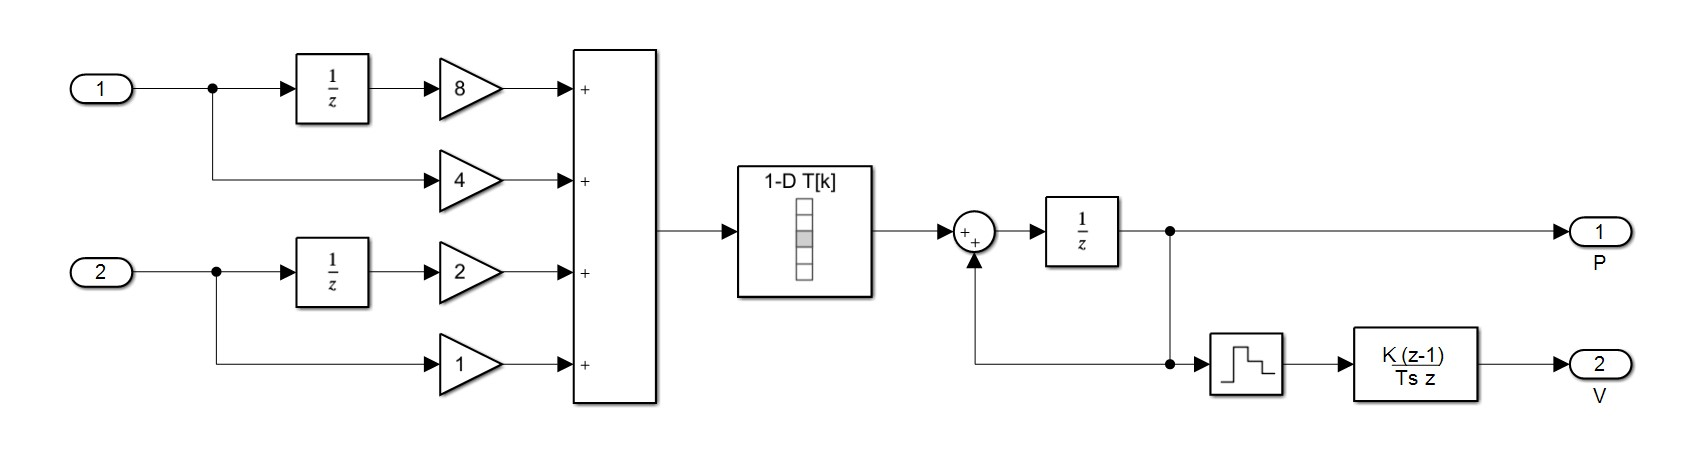
\includegraphics[width=\textwidth]{la3.jpg}
\caption{Estructura del bloque Lector Encoder}
\label{f20}
\end{figure} 
Para entender mejor su funcionamiento vamos a describir primero el algoritmo empleado. Como se explicó en la sección \ref{s111} al describir el motor, éste emplea un par de encoders en cuadratura, configurados de tal modo que, cada vez que se cruza un flaco de subida o bajada de uno de los encoders, el eje de la reductora ha avanzado un grado.

Supongamos que fijamos un tiempo de muestreo y vamos midiendo regularmente los valores de los enconders. Comparando la lectura de los encoders en dos instantes de muestreo consecutivos podemos deducir si el motor a avanzado un pulso de encoder y en qué dirección. Si nos fijamos en la figura \ref{f6bis} en que se  representan de nuevo las señales de los encoders, es fácil entender lo que se quiere decir: cada vez que un encoder cruza un flanco, cambia la lectura del encoder correspondiente, y podemos considerar que el motor a avanzado un grado. Así por ejemplo, en el instante $t=0$ de la figura la lectura de los dos encoders es $encoderA(0) = 0, encoderB(0) = 0$ y seguirá así hasta el instante $t \approx 1.02$ en que la las lecturas cambiarán a $encoderA(1.02) = 1, encoderB(1.02) = 0$. Podemos construir, a partir de las lecturas en dos instantes de muestreo sucesivos, un registro de cuatro dígitos en el que, a medida que vamos obteniendo nuevas lecturas, actualizamos el valor de los registros, de modo que guardamos la última lectura realizada por los encoders y la realizada en el instante de muestreo anterior. 
\begin{figure}
\centering
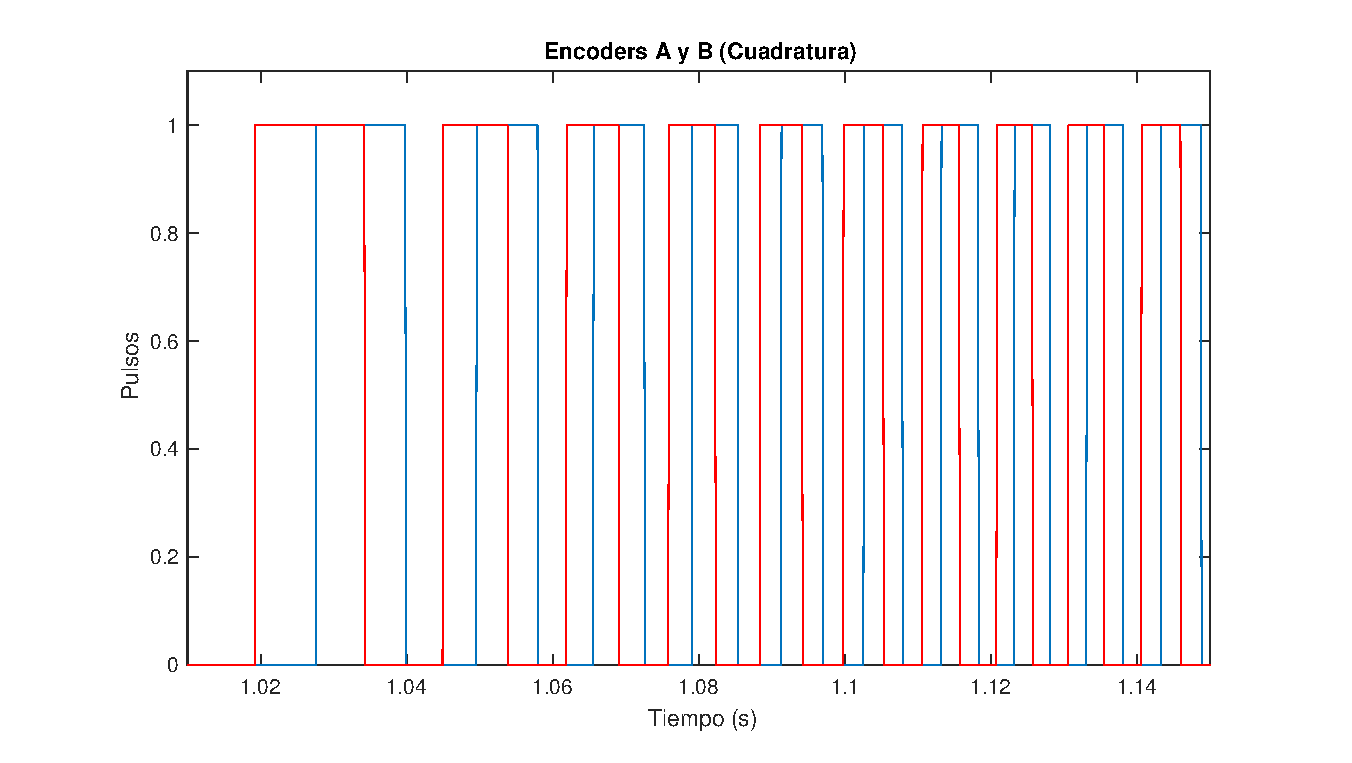
\includegraphics[width= 0.7\textwidth]{encoderab.eps}
\caption{Señales producidas por un encoder en cuadratura al girar el motor }\label{f6bis}
\end{figure} 
Así en el caso de la figura \ref{f6bis} y suponiendo un periodo de muestreo de los valores de los encoder de 0.01s, obtendríamos una secuencia de valores:
\begin{align*}
encoderA(0.00) = 0, encoderA(0.01) = 0,encoderB(0.00) = 0, encoderB(0.01) = 0\\
encoderA(0.01) = 0,encoderA(0.02) = 0,encoderB(0.01) = 0, encoderB(0.02) = 0\\
encoderA(0.02) = 0,encoderA(0.03) = 0,encoderB(0.02) = 0, encoderB(0.03) = 0\\
\cdots \\
encoderA(1.01) = 0,\mathbf{encoderA(1.02) = 1},encoderB(1.01) = 0, encoderB(1.02) = 0\\
encoderA(1.02) = 1,encoderA(1.03) = 1,encoderB(1.02) = 0, encoderB(1.03) = 0\\
\cdots
\end{align*}

Esta información se podría codificar como un registro de 4 bits, correspondientes a los valores 1/0 de la señal de los encoders. Su estructura y los valores posibles se muestran en la tabla \ref{t3}. Los valores positivos corresponden a un avance de un pulso (1 grado) entre los dos últimos instantes de muestreo. Los negativos indican que el motor ha retrocedido un grado, los ceros indican  que el motor no se ha movido. Por último, los valores marcados con 'NA' (No Aplicable) indican situaciones imposibles, nunca se dará dicho cambio en la lecturas de los encoders, siempre y cuando el periodo de muestreo elegido se menor que la mitad del tiempo de paso por dos flancos consecutivos de los encoders.

En la última columna de la tabla se ha indicado el valor en decimal que correspondería al registro de cuatro bits que forman los valores de los encoders:
\begin{equation}\label{eq1}
Dec = 2^3\cdot EncoderA(i-1)+2^2\cdot EncoderA(i)+2^1\cdot EncoderB(i-1)+2^0\cdot EncoderB(i)
\end{equation}

Pasar el número a decimal nos permite codificar los valores en una tabla de modo bastante sencillo en Simulink
\begin{table}
\centering
\begin{tabular}{c c c c c c}
\multicolumn{2}{c}{\textbf{Encoder A}}&\multicolumn{2}{c}{\textbf{Encoder B}}&Pulso&Dec.\\
\hline
$T = i-1$&$T =i$&$T = i-1$&$T =i$& &\\
0&0&0&0&0&0\\
0&0&0&1&-1&1\\
0&0&1&0&+1&2\\
0&0&1&1&0&3\\
0&1&0&0&+1&4\\
0&1&0&1&NA&5\\
0&1&1&0&NA&6\\
0&1&1&1&-1&7\\
1&0&0&0&-1&8\\
1&0&0&1&NA&9\\
1&0&1&0&NA&10\\
1&0&1&1&+1&11\\
1&1&0&0&0&12\\
1&1&0&1&+1&13\\
1&1&1&0&-1&14\\
1&1&1&1&0&15\\
\hline
\end{tabular}
\caption{Tabla de lectura para los encoders. El signo indica el sentido en que ha girado el motor, Dec es el núnero decimal representado por los 4 bits del registro}\label{t3}
\end{table}

Volvamos ahora a la figura \ref{f20} y examinemos los bloque de Simulink empleados.

En primer lugar las entradas 1 y 2 alimentan a un bloque \emph{unit delay} de la librería Simulink/discrete. Este bloque representa un retardo puro, es decir, devuelve el valor del encoder A en el instante de muestreo anterior al actual. Además, las salidas están conectadas a ganancias de valores 8, 4 , 2 y 1, y las salidas de las ganancias están conectadas a un bloque sumador. Es fácil darse cuenta que el resultado de dicha operación arrojará el valor decimal correspondiente al registro de los valores de los encoders, que acabamos de describir (eq \ref{eq1}).

La salida del sumador alimenta un bloque \emph{Direc look-at table} de la librería Simulink/look-at table. Se trata de un bloque muy sencillo. El parámetro de configuración es, en nuestro caso, un simple array con los valores correspondientes a la columna pulso de la tabla \ref{t3}, escritos por orden:
\begin{verbatim}
[0,-1,1,0,1,0,0,-1,-1,0,0,1,0,1,-1,0]
\end{verbatim}
Donde hemos sustituido por 0 los valores NA. El bloque espera  en su entrada un número de índice para el array, contrariamente a lo que es habitual en Matlab, los índices empiezan en 0 y  no en 1. La tabla devuelve a la salida el valor del array correspondiente al valor de la entrada. Así, para una entrada 0 devolvería un 0 para una entrada 1 devolvería un -1, etc.

Como la entrada a este bloque debe ser un índice, es preciso fijar el tipo de variable para la salida del bloque anterior (sumador). Para ello, basta hacer doble 'click' en el bloque sumador, seleccionar la pestaña \emph{signal attributes} y en el menú desplegable \emph{output data type} seleccionar la opción 'double'. 

La salida de la tabla está conectada a un bloque \emph{Unit delay} Realimentado, Cada vez que se obtiene un nuevo valor en la tabla, se suma a los valores anteriores, de modo que el lazo actúa como un acumulador de pulsos, la salida será directamente la posición en grados del eje de la reductora del motor.

Por último, la salida del bloque \emph{Unit delay} está también conectada a un bloque \emph{Zero-Order Hold} (retenedor de orden 0) de la librería Simulink/discrete. Este bloque lleva su propio periodo de muestreo que, en nuestro caso hemos fijado en 0.01. El bloque toma una lectura de la entrada ---en este caso la posición calculada a partir de los encoders--- y retiene su valor durante el periodo de muestreo. El bloque alimenta a su vez a un bloque \emph{discrete time derivative} de la librería Simulink/discrete que estima la derivada de la posición y por tanto la velocidad. Se trata en realidad de una aproximación un tanto imprecisa que necesitaría de un posterior filtrado. Pero para una primera aproximación nos puede valer.

\paragraph{Practica 1}
\begin{enumerate}
\item Identificar todos los componentes de la planta. Placa de desarrollo, Placa de expansión, Motor, Fuente de alimentación, etc.
\item Comprobar que todo el \emph{Hardware} está configurado de acuerdo a la descripción de estas notas.
\item Montar el modelo de Simulink para el manejo del motor en lazo abierto. Configurarlo y comprobar que funciona correctamente, haciendo que el motor se mueva.
\item Recoger datos de velocidad y posición para diversos valores del voltaje de entrada. Observar también las señales de los encoders y discutir su validez. 
\end{enumerate}


\section{Modelo e identificación del motor}

\begin{figure}[h]
\centering
\begin{circuitikz}
\draw(0,2)to[battery1=$K_Ae(t)$](0,-1)to[short](4,-1);
\draw (0,2) to[R=$R_0$,i=$i(t)$] (2,2) to[R=$R$] (4,2);
%\draw (0,0) to[short, o-*] (2,0) to[short, -*] (3.5,0) to[short] (5,0);
\draw (4,2) to[L=$L$] (4,0.5);
\draw (4,0.5) to[sV, color=white, name=M2] (4,-1);
\mymotor{M2}{90}
%
\draw[latex-] (4.3,-1) arc (-70:70:0.8);
\draw(5.4,-0.25)node{$\theta(t)$};
\end{circuitikz}
\caption{Circuito equivalente para un motor de continua}\label{f21}
\end{figure}

\paragraph{Modelo del motor} El circuito de la figura \ref{f21} representa un motor de corriente continua y su sistema de alimentación. Podemos considerar el sistema compuesto de dos partes:

\begin{itemize}
	\item Una parte eléctrica formada por un variador (Puente en H más señal de PWM)  que recibe un voltaje de entrada $e(t)$ y devuelve un voltaje amplificado $K_Ae(t)$. Además el amplificador tiene una resistencia interna $R_0$.

 La parte eléctrica del motor (bobinado) viene representada por una autoinductancia $L$ y una resistencia $R$. Por último, podemos considerar que la caída de tensión (fuerza contra electromotriz) debida al giro del motor es proporcional a la velocidad angular $\dot{\theta}$ con la que gira el rotor.  La constante de proporcionalidad $a$ depende de las características del motor. Si sumamos todas las caídas de tensión en el circuito:


\begin{equation}\label{elc}
L\frac{di(t)}{dt}+(R+R_0)i(t)+a\frac{d\theta(t)}{dt} = K_Ae(t)
\end{equation}

\item Una parte mecánica que podemos asociar al momento de inercia $J$ del rotor y  a la resistencia al giro ofrecida por el rozamiento --que consideraremos proporcional a la velocidad angular a través de un coeficiente de rozamiento viscoso $\mu$. 

El par ejercido por el motor, es proporcional a la intensidad que circula por el bobinado. La constante de proporcionalidad vuelve a ser la constante del motor $a$. Por último, podemos suponer que la carga que mueve el motor ejerce un par $T_L$:

\begin{equation}\label{mec}
J\frac{d^2\theta(t)}{dt^2}+\mu\frac{d\theta(t)}{dt} = ai(t)-T_L(t)
\end{equation}
\end{itemize}
Sin embargo, la dinámica debida a la autoinducción $L$ es mucho más rápida que la dinámica propia de la mecánica del motor.  Esto nos permite simplificar el modelo eliminando la variación de la intensidad --es tán rápida que el resto del sistema siempre la \emph{ve} en su estado estacionario--.

 \begin{equation}\label{sim}
L\frac{di(t)}{dt}= 0 \Rightarrow (R+R_0)i(t)+a\frac{d\theta(t)}{dt} = K_Ae(t)
\end{equation}

Si despejamos la intensidad de la ecuación \ref{sim} y sustituimos en \ref{mec}, obtenemos:

\begin{equation}\label{s}
J\frac{d^2\theta(t)}{dt^2}+\left(\mu+\frac{a^2}{R+R_0}\right)\frac{d\theta(t)}{dt} = \frac{aK_A}{(R+R_0)}e(t)-T_L(t)
\end{equation}

La ecuación anterior la podríamos reescribir como un modelo en representación en variables de estados con dos estados $\theta$ y $\omega= \dot{\theta}$ 

\begin{align}
\dot{\theta}(t) &= \omega(t)\\
\dot{\omega}(t) &=-\frac{1}{J}\left(\mu+\frac{a^2}{R+R_0}\right)\omega(t)+\frac{1}{J}\frac{aK_a}{(R+R_0)}e(t)-\frac{1}{J}T_L(t)\\
\end{align}



Alternativamente, si obtenemos la transformada de Laplace de la ecuación \ref{s}, tendríamos dos funciones de transferencia una para la relación tensión-posición y otra para la relación par de carga-posición:

\begin{equation}
\theta(s) = \frac{1}{s}\frac{\frac{1}{J}\frac{aK_A}{R+R_0}}{s+\left(\mu+\frac{a^2}{R+R_0}\right)\frac{1}{J}}e(s)-\frac{1}{s}\frac{\frac{1}{J}}{s+\left(\mu+\frac{a^2}{R+R_0}\right)\frac{1}{J}}T_L(s)
\end{equation}

En la mayoría de los casos desconocemos los valores de las parámetros del motor. Sin embargo, los agrupamos en tres simples constantes, que podemos estimar experimentalmente:
\begin{equation}
k_e = \frac{1}{J}\frac{aK_A}{R+R_0},\ p = \left(\mu+\frac{a^2}{R+R_0}\right)\frac{1}{J},\ k_m = \frac{1}{J}
\end{equation}
 
Si, además consideramos un par de carga nulo $T_L(t) = 0, \forall t$, los modelos se simplifican pasando a ser modelos SISO:

\begin{align} \label{eq311}
\begin{bmatrix}
\dot{\theta}\\
\dot{\omega}
\end{bmatrix} &= \begin{bmatrix}
0 & 1\\
0 &-p
\end{bmatrix}\cdot\begin{bmatrix}
\theta\\
\omega
\end{bmatrix}+\begin{bmatrix}
0\\
k_e
\end{bmatrix}e(t)\\ \label{eq312}
y &= \begin{bmatrix}
1& 0
\end{bmatrix}\cdot\begin{bmatrix}
\theta\\
\omega
\end{bmatrix}
\end{align} 

\begin{equation}
\theta(s) = \frac{k_e}{s(s+p)}e(s)
\end{equation}

\begin{figure}
	\centering
	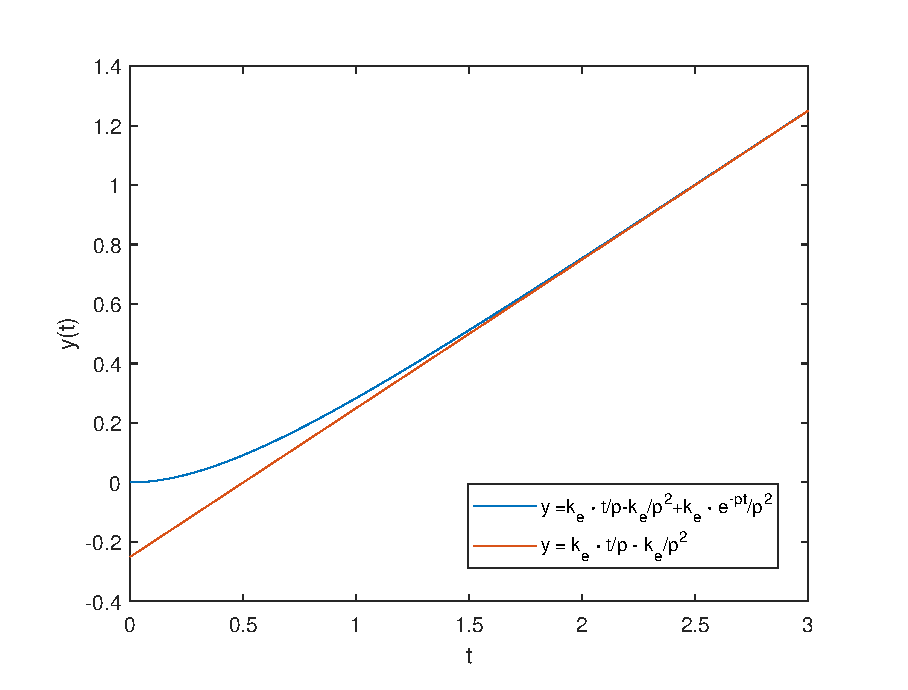
\includegraphics[width=0.8\textwidth]{resq.eps}
	\caption{Respuesta de un motor de cc a un voltaje de entrada escalón}\label{f22}
\end{figure}

\paragraph{Identificación del motor} Si calculamos la respuesta de nuestro sistema a una entrada escalón de valor $e(t) = V$,
\begin{equation}\label{eq314}
\theta(t) = V\frac{k_e}{p^2}e^{-pt}+V\frac{k_e}{p}t -V\frac{k_e}{p^2} 
\end{equation}



La respuesta angular en estado estacionario es una línea recta, que indica que el motor, tras pasar la fase transitoria, gira con velocidad constante. La figura \ref{f22} muestra un ejemplo de la respuesta de un motor como el que estamos modelando. Si obtenemos la pendiente de la recta correspondiente a la solución estacionaria y su corte con el eje $y$, podemos estimar los parámetros $K_e$ y $p$ de nuestro motor. Este proceso puede hacerse a partir de datos experimentales del motor, en cuyo caso recibe el nombre de proceso de identificación del motor.


\paragraph{Práctica 2}
\begin{enumerate}
\item Obtener a partir de cálculo simbólico la expresión correspondiente a la posición angular de un motor de continua (ecuación \ref{eq314}). Obtenerla a partir del modelo en variables de estado y a partir de la función de transferencia. Calcular también la expresión correspondiente a la velocidad angular.
\item Construir un modelo del motor de cc en Simulink. Se puede hacer a partir de las ecuaciones de estado o de funciones de transferencia, pero de modo que se pueda obtener tanto la posición como la velocidad angular. El modelo deberá obtener los parámetros $k_e$ y $p$ del \emph{workspace} de Matlab.
Emplear el modelo de Simulink para el control del motor, construido en la práctica anterior, en lazo abierto para identificar el motor real. Es decir para obtener sus parámetros $k_e$ y $p$. Para ello:
\begin{itemize}
\item Obtener la respuesta del motor para distintos voltajes (por ejemplo incrementando el valor de la entrada de dos voltios en dos voltios desde 0 a 12V) y un tiempo de simulación en todos los casos de 3s.
\item Calcular por regresión lineal la pendiente y el término independiente de la respuesta en estado estacionario.
\item Estimar los valores de Ke y p para cada valor del voltaje de entrada ¿Qué se puede concluir?
\end{itemize} 
\item Introducir los valores obtenidos de Ke y p en el modelo de motor desarrollado en Simulink (obtener unos valores promedio razonables) Comparar los resultados del modelo con el sistema real.
\end{enumerate}

\chapter{Control del motor por realimentación de estados estimados}
En esta sección vamos a construir un regulador completo para controlar la posición del motor. Empezaremos construyendo un modelo realista completo del sistema, a partir de los datos obtenidos en el proceso de identificación del capítulo anterior.

\section{Un modelo completo del motor}\label{sec41}

\paragraph{Modelo ideal del motor} Vamos a construir un modelo del motor que emplee exactamente las mismas señales de entrada y salida que emplea el motor real. Además, tendremos en cuenta algunas de las no linealidades más características: la existencia de un voltaje máximo que no se puede superar y la existencia de un voltaje mínimo por debajo del cual el motor no funciona.

\begin{figure}[h]
\centering
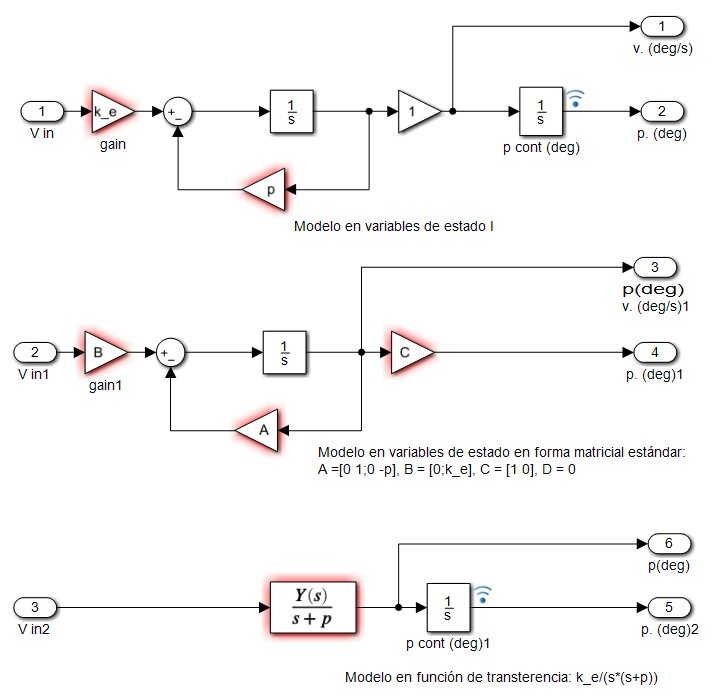
\includegraphics[scale=0.8]{modelo_motor1.jpg}
\caption{Esquemas de Simulink para el modelo del motor ideal}
\label{f23}
\end{figure}

La figura \ref{f23} muestra tres versiones del modelo sencillo descrito en la sección anterior para un motor ideal de corriente continua. Las dos primeras son  versiones en variables de estados y la tercera una versión empleando la función de trasferencia. Los tres modelos son equivalentes y cualquiera de ellos se puede usar como núcleo de un modelo más realista del motor que estamos empleando. El modelo basado en la función de transferencia emplea en realidad dos en cascada. La razón es tener acceso no solo a la posición --que es la salida del sistema-- sino también a la velocidad que corresponde a la salida de la primera función de transferencia. Para ajustar nuestro modelo al motor real empleado en la práctica, deberemos ajustar los valores de \emph{Ke} y \emph{p} a los valores obtenidos en el proceso de identificación del motor, descrito en el apartado anterior. Se ha añadido una ganancia a la salida del modelo que podría ajustarse para modelar la reductora. Se trata tan solo de una constante y dado que hemos identificado el motor empleando la posición del eje de la reductora, podemos asignarle directamente valor $1$. 

\paragraph{Modelo del sistema de alimentación} Para aproximar nuestro modelo al motor de la práctica, el siguiente paso es construir un modelo de su sistema de alimentación. Sabemos que el motor recibe un nivel de tensión variable mediante el empleo de una señal de PWM. Para emular dicho sistema, creamos un nuevo modelo de Simulink como el que se muestra en la figura \ref{f24}. El modelo se construye a partir de un bloque que reproduce una señal en diente de sierra, construido a partir de un bloque \emph{Repeating Sequence} de la librería Simulink/Sources. Este bloque espera como parámetros un vector de instantes de tiempo (\emph{Time values}) comprendidos entre $0$ y un tiempo final $T$, y un vector de valores de salida (\emph{Output values}) de la misma longitud que el vector de tiempos. El módulo, durante su ejecución, da como salida la secuencia introducida repetida periódicamente cada $T$ segundos. En nuestro caso empleamos los siguientes vectores como parámetros:
\begin{verbatim}
Time Values: linspace(0,T,100)
Output values: linspace(0,Vmax,100)
\end{verbatim}

El resultado de la señal de salida del bloque será una sucesión de valores crecientes entre $0$ y Vmax, que se repiten periódicamente cada T segundos. La señal toma por tanto la forma de un diente de sierra. El bloque comparador compara el valor de entrada, Vref,  en cada instante con el valor de el diente de sierra. Vref representa el valor de tensión continua que queremos emular con la señal de PWM. Mientras el valor del diente de sierra sea menor que el de la entrada Vref, la comparación devuelve un $1$, en caso contrario devolverá un $0$. La ganancia multiplica el 1 o el 0, por el valor Vmax. El resultado es que a la salida tendremos un valor igual a Vmax durante un periodo igual al que la entrada es mayor que el valor del diente de sierra, y a partir de ahí y hasta el final de periodo T, valdrá cero. Es fácil comprobar que la señal así construida corresponde a una señal de PWM de valor Vmax y periodo T. El tiempo que la señal está activada (\emph{duty cicle}) corresponde precisamente al tiempo en que la entrada supera en valor a la señal en diente de sierra. Así por ejemplo, si elegimos $\text{Vref} = \text{Vmax}/2$ la señal valdrá Vmax durante un tiempo $t=\text{Vmax}/2$.  
\begin{figure}
\centering
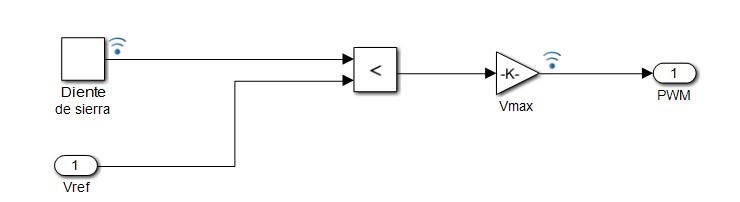
\includegraphics[scale=1]{pwm_gen.jpg}
\caption{Esquema de Simulink del bloque construido para generar una señal de PWM}
\label{f24}
\end{figure}
Podemos enmascarar todo el modelo de la figura \ref{f24} en único bloque y definir como parámetros Vmax y T. 

Un detalle importante a la hora de manejar el bloque de PWM descrito tiene que ver con el modo en que Simulink maneja los tiempos de los modelos. Por defecto, Simulink emplea integradores de tiempo variable, de modo que el tiempo entre pasos de integración se ajusta a la convergencia de las soluciones del modelo. En nuestro caso, podría suceder que los pasos empleados por Simulink sean tan grandes que nos recorte la señal de PWM. Para evitar esto es importante ajustar el paso máximo de integración, en el modelo en que se está empleando el bloque PWM, a la décima parte (o menor) que el periodo T asignado a la señal de PWM. El ajuste se hace en la ventana \emph{Parameter configuration}, \emph{Max step size}. Un valor razonable para un $\text{T} = 0.001s$ sería \emph{Max step size} $=1e-5$  
Por último podemos probar el funcionamiento del bloque para varios valores de entrada. Las figuras \ref{f25a} y \ref{f25b} muestran el nuevo bloque construido y su salida  comparada con la señal en diente de sierra, y el voltaje de referencia, para valores $\text{Vmax }= 12$ y $\text{T} = 0.001$ y un valor $\text{Vref} =0.5$ 

\begin{figure}
\centering
\begin{subfigure}{0.5\textwidth}
\includegraphics[scale=0.3]{pwm_pr.jpg}
\caption{Bloque desarrollado y ventana de parámetros}
\label{f25a}
\end{subfigure}
\begin{subfigure}{0.5\textwidth}
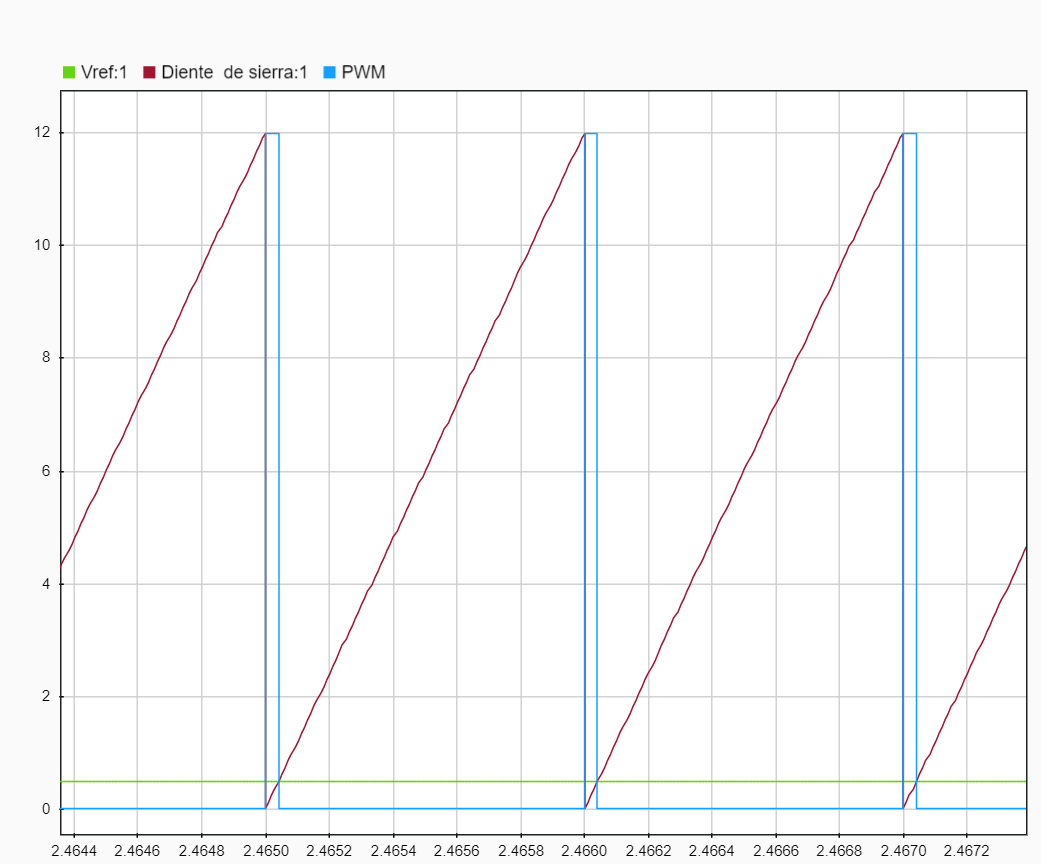
\includegraphics[scale=0.5]{pwm_gen.png}
\caption{Señales empleadas en el generador de PWM}
\label{f25b}
\end{subfigure}
\caption{Bloque para simular una señal de PWM}
\end{figure}

Es interesante hacer notar que el bloque construido, --al igual que pasa con el controlador real-- no permite alimentar el motor con un voltaje mayor que el voltaje de la fuente de alimentación. Además, al dar solo valores positivos, solo permitiría mover el modelo del motor en un sentido de giro. 

Nos faltaría emular el efecto del puente en H. Para ello, añadimos al modelo construido los siguientes bloques de la librería \emph{Simulink/Math operations}: Un bloque \emph{Abs}, que obtenga el valor absoluto de la señal Vref. Un bloque \emph{sign}, que extraiga el signo el signo de la señal Vref. Un bloque \emph{Prod} que multiplique la salida del bloque PWM por el signo de la seña Vref. El modelo resultante se muestra en la figura \ref{f26} Es fácil comprobar que si introducimos una señal Vref negativa, la señal de PWM a la salida, será negativa, emulando así el efecto del cambio de entradas de un puente en H.
\begin{figure}
\centering
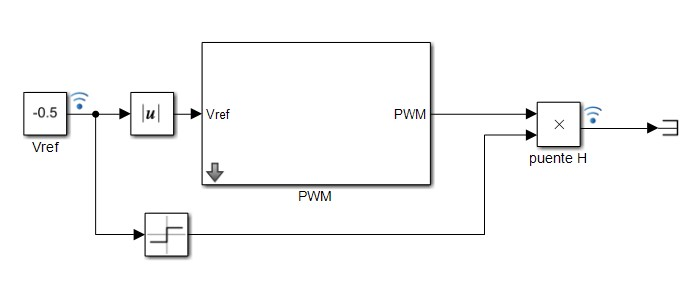
\includegraphics[scale=1]{puenteH.jpg}
\caption{Modelo del alimentador de tensión al motor incluyendo el cambio de signo de voltaje.}
\label{f26}
\end{figure}

Una vez construido el sistema de alimentación del motor, podemos crear un modelo que incluya tanto la alimentación como el modelo de motor ideal, empleando cualquiera de los esquemas de Simulink de la figura \ref{f23}. La figura \ref{f27} muestra un ejemplo. En este caso, se ha optado por emplear el primero de los modelos en variables de estado de la figura \ref{f23}. El modelo del motor se ha enmascarado definiendo como parámetros del modelo las constantes $p$ y $Ke$. Se han conservado como variables de salida la posición y velocidad (angulares) del eje del motor. Aunque dichas variables se han etiquetado como \emph{p(rad)} y \emph{v (rad/s}) las unidades dependen en realidad del valor que se asigne a las constantes del modelo. Se ha añadido a la entrada del modelo un bloque \emph{dead zone} de la librería \emph{ Simulink/discontinuities}. Este bloque sirve para simular la zona muerta del motor; es decir, el voltaje mínimo por debajo del cual el motor no se moverá. Estrictamente debería ir en el bloque que simula el motor, pero esto complica el modelo. En realidad, la señal de PWM siempre da al motor el voltaje máximo, lo que realmente limita es la corta duración del \emph{duty cycle} cuando el voltaje de referencia es muy bajo. Modelarlo exactamente ralentiza enormemente el tiempo de integración y genera errores de precisión. La forma en que se ha modelado dará valores razonables, siempre que el periodo de la señal de PWM sea razonablemente corto.

\begin{figure}
\centering
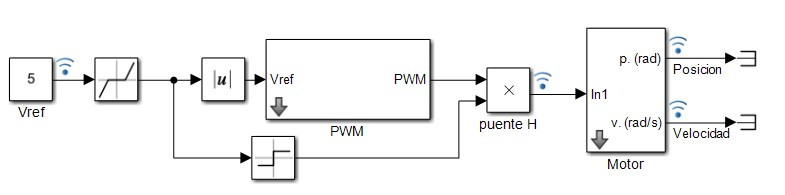
\includegraphics[width=0.8\textwidth]{pwm_motor.jpg}
\caption{Esquema del modelo incluyendo el motor y su sistema de alimentación}
\label{f27}
\end{figure}  

\paragraph{Modelado de los encoders} Una vez modelados el motor y su sistema de alimentación, debemos modelar también el comportamiento de los \emph{encoders}. Como se ha descrito en las secciones anteriores, el motor real dispone de dos \emph{encoders} en cuadratura que suninistran un pulso --flanco de subida y bajada-- por cada grado que avanza el eje del motor. Podemos diseñar un modelo para ellos que utilice como entrada la salida del modelo ideal del motor. Como los \emph{encoders} están situados en cuadratura, la distancia recorrida por el motor entre un flanco de subida y bajada de un \emph{encoder} es de 2 grados. Además las lectura están entrelazadas. Entre flancos, cada \emph{encoder} deberá dar un valor constante -- $1$ ó $0$ -- dependiendo de la posición del eje del motor. La figura \ref{f28} ofrece un posible modelo para los \emph{encoders}.
\begin{figure}[h]
\centering
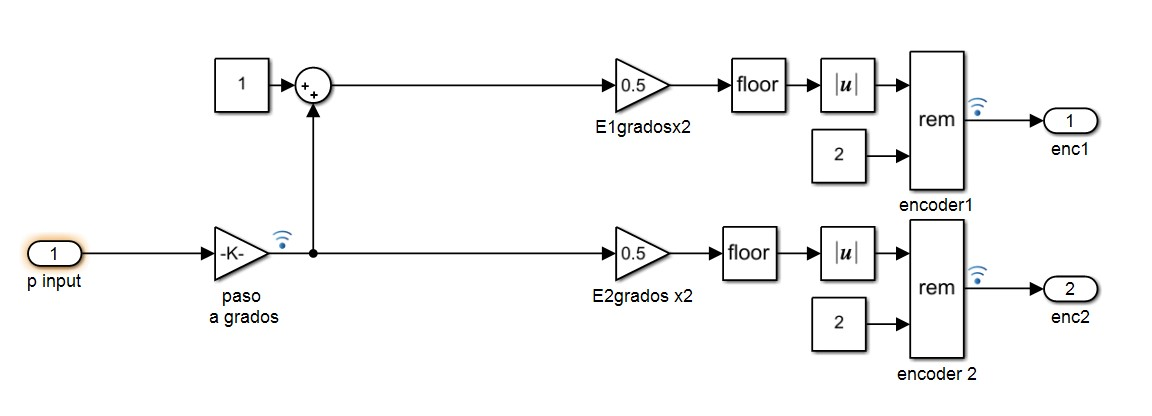
\includegraphics[width=\textwidth]{m_encoder.jpg}
\caption{Modelo de Simulink para dos \emph{encoders} en cuadratura}
\label{f28}
\end{figure}

El modelo toma como entrada la salida del modelo del motor ideal, correspondiente a la posición angular del eje. La ganancia etiquetada como \emph{paso a grados} solo se emplea si la salida del motor se mide en radianes, si se mide en grados tomará valor 1. Se han introducido dos bloque no empleados anteriormente, pertenecientes a la librería \emph{Simulink/math operations}. Se trata del bloque \emph{floor} que redondea un numero hacia cero y el bloque \emph{rem} que calcula el resto de la división entera de la entrada superior entre la entrada inferior.

Para analizar su funcionamiento, consideremos el motor parado al inicio de una simulación, El valor de la posición \emph{p input} del eje del motor es $0$. El camino que lleva a la salida \emph{enc1} corresponder al \emph{encoder} A. El modelo suma un 1 constante a dicho valor y divide el resultado por dos. Tras el redondeo hacia cero, y el cálculo del resto de la división entre  dos, el valor de la salida será 0. La salida \emph{enc2}, correspondiente al \emph{encoder} B, también tomará valor cero. Supongamos que avanza un grado la posición del eje del motor, la lectura del \emph{encoder} A cambiará a 1, mientras que la del \emph{encoder} B seguirá siendo cero. Si el motor avanza un grado más, la lectura de A se mantiene en su valor 1, y la de B pasará a valer 1. Es fácil observar que, en el periodo comprendido entre incrementos de un grado, ambos \emph{encoders} mantendrán constante su valor de salida y que la secuencia temporal de ambas señales reproduce la que cabría esperar para dos \emph{encoders} en cuadratura. Para probarlo, podemos encapsular nuestro modelo en un bloque, conectar su entrada a la salida del modelo del motor y simular el modelo completo. Las figuras \ref{f29a} y \ref{f29b} muestran el modelo completo y las señales de salida obtenidas para los \emph{encoders}.

\begin{figure}
\centering
\begin{subfigure}{\textwidth}
\centering
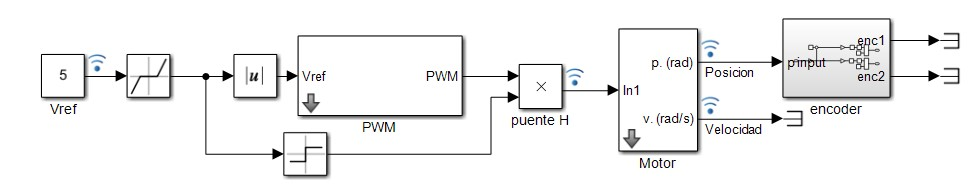
\includegraphics[width=\textwidth]{motor_encoders.jpg}
\caption{Modelo del motor incluyendo el bloque del modelo de los encoders}
\label{f29a}
\end{subfigure}
\begin{subfigure}{\textwidth}
\centering
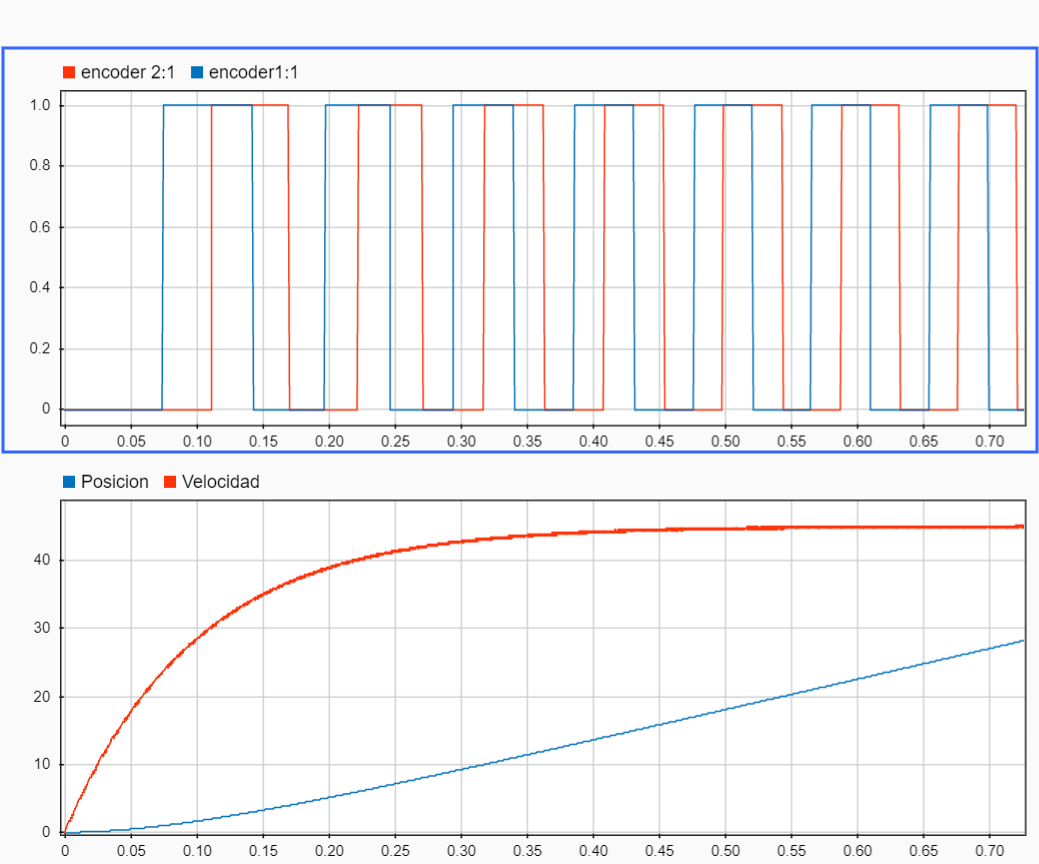
\includegraphics[scale=0.5]{encoders.png}
\caption{Modelo del motor incluyendo el bloque del modelo de los encoders}
\label{f29b}
\end{subfigure}
\caption{Modelo completo del motor}
\end{figure}

Con todos los elementos anteriores hemos construido un modelo completo del motor. Podemos alimentarlo con un voltaje de referencia y obtener los valores que nos darían las lecturas de sus encoders. Por último podríamos emplear el mismo bloque \emph{lector encoders} descrito en la figura \ref{f20} para leer los pulsos del bloque \emph{encoder} y obtener los valores de la posición angular y la velocidad del eje de la reductora del motor. Podemos además comparar dichas salidas con las que suministra el bloque \emph{motor} que hemos construido y ver el efecto de la cuantización y el muestreo sobre las salidas del motor. La figura \ref{f30} muestra un ejemplo en que se comparan dichas salidas. Se ha buscado un caso en el que se notan especialmente estos efectos. Así, los escalones en la lectura de la posición realizada con los \emph{encoder} son claramente visible en la parte superior de la figura. Además se ha elegido un tiempo $\Delta t = 1s$ en que se observa claramente el efecto del retenedor de orden cero sobre la medida de la velocidad. El algoritmo empleado para estimar la medida de la velocidad es sencillo, pero no es nada robusto. El motor alcanza su velocidad estacionaria en menos de $1s$ pero el lector no es capaz de detectarlo. Una vez alcanzada dicha velocidad, el lector oscila por encima y por debajo del valor real. Si disminuimos el valor de $\delta T$, esta oscilación se hará aún más acusada. Si lo aumentamos, acumularemos aún un retardo mayor en la detección de los cambios de velocidad. No podemos por tanto emplear esta medida directamente para controlar el motor.

\begin{figure}
\centering
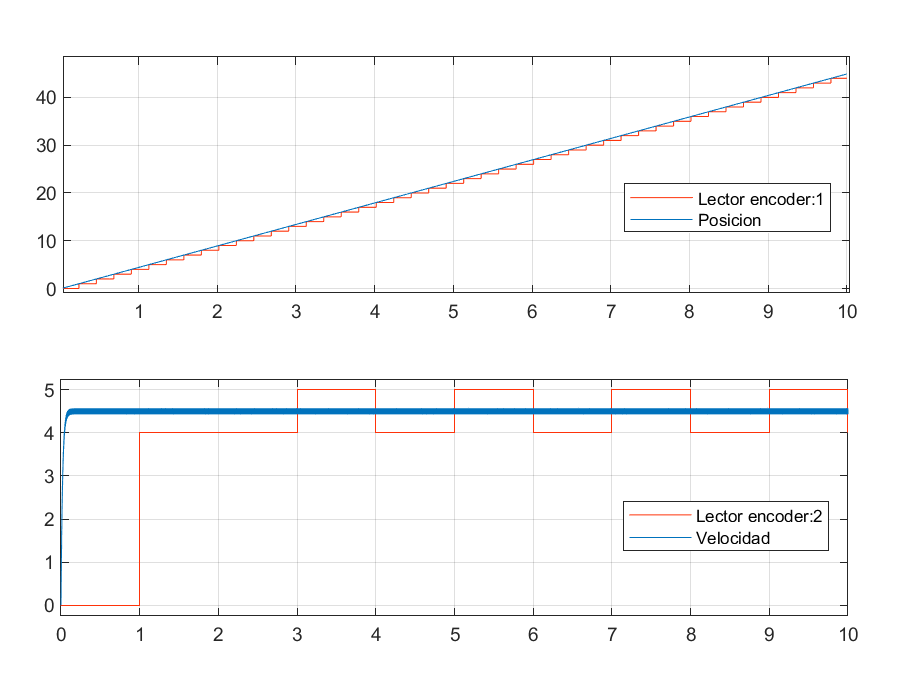
\includegraphics[scale=0.6]{salida_modelo.eps}
\caption{Comparación entre las variables de salida posición y velocidad obtenidas por el modelo del motor y el valor de dichas variables obtenidas a partir de la lectura de los \emph{encoders}}
\label{f30}
\end{figure}

\paragraph{Práctica 3}
\begin{enumerate}
\item Construir un modelo completo del motor, a partir del modelo de motor ideal construido en la Práctica 2. Añadir el mismo bloque de lectura de \emph{encoders} construido para leer los \emph{encoders} del motor real.

\item Simular el comportamiento del modelo para distintos valores del voltaje de entrada Vref. 
\begin{itemize}
\item Comparar la salida directa (posición y velocidad) del motor con la que se obtiene a partir de la lectura de los \emph{encoders}
\item Comparar los valores de las lecturas de velocidad y posición obtenidas a través de los \emph{encoders} para el motor real y para el modelo.
\end{itemize}
\end{enumerate}

\section{Diseño de un controlador de la posición del motor por realimentación de estados estimados}
\subsection{Controlador para el motor ideal}
Para estudiar el diseño del controlador, empezaremos considerando el motor ideal en variables de estado descrito por las ecuaciones \ref{eq311}, \ref{eq312}. El objetivo final es desarrollar un controlador de posición angular del eje del motor. Si trabajamos sobre el modelo del motor ideal, podemos empezar analizando su estabilidad. Si calculamos los autovalores de la matriz del sistema (\ref{eq311}),
\begin{equation}
A = \begin{bmatrix}
0 & 1\\
0 &-p
\end{bmatrix}, \vert \lambda I-A\vert = 0 \rightarrow \lambda_1 = 0, \lambda_2=-p
\end{equation}

El sistema tiene un polo real negativo y un polo en el origen. Lo que corresponde al comportamiento físico observable. Si suministramos una entrada escalón (Vref = cte) el motor se mueve indefinidamente con velocidad constante. 

\paragraph{Realimentación de estados.} Podemos empezar por diseñar un controlador por realimentación de estados, para mover los polos del sistema.  Podemos emplear para calcular las ganancias de la realimentación cualquiera de las funciones definidas en Matlab para este propósito: \texttt{acker} o \texttt{place}. Aunque teóricamente los polos pueden situarse en cualquier lugar del semiplano negativo complejo, hay que tener en cuenta que cuanto más a la izquierda los situemos más grande será el valor de la variable (Vref) demandada por el motor durante el transitorio. Por otro lado, si elegimos polos cercanos al eje imaginario, la respuesta del sistema puede ser muy lenta  y demandar tensiones tan bajas que el motor real entre en su zona muerta y no alcance el estado estacionario. Un posible ajuste inicial, puede ser, situar ambos polos relativamente cerca del valor $p$ obtenido para el polo $p$ del motor durante la identificación realizada en las prácticas anteriores. Por ejemplo podemos calcular cuáles serían las ganancias $k = [k_1, k_2]$ de la realimentación de estados si situamos los polos en $p_1 = 0.5p$ y $p_2 = 0.5p$\footnote{Si colocamos ambos polos en la misma posición será preciso emplear \texttt{acker} para obtener las ganancias}. Podemos además obtener la evolución de los estados si partimos del modelo de motor ideal que diseñamos en la práctica anterior.  

La figura \ref{f31b} muestra los resultados de un ejemplo de dicho sistema. Se ha considerado la posición inicial del motor $x_1 = 2^o$ y la velocidad inicial $x_2= 1^o/s$.  Los valores $K_e = 100$ y $p = 50$ se han tomado arbitrariamente y  no tienen por qué corresponder con los del motor estimado (De hecho $K_e$ para el motor real es un orden de magnitud mayor). La entrada con el bloque escalón se ha puesto a cero. La señal $u$ representaría en este modelo el voltaje Vref. suministrado al motor. La realimentación de estados diseñada es capaz de llevar el motor a su posición cero, como era de esperar. Dado que hemos fijado la entrada a cero, la realimentación de estados está respondiendo exclusivamente a los valores iniciales de los estados del sistema.
\begin{figure}
\centering
\begin{subfigure}{\textwidth}
\centering
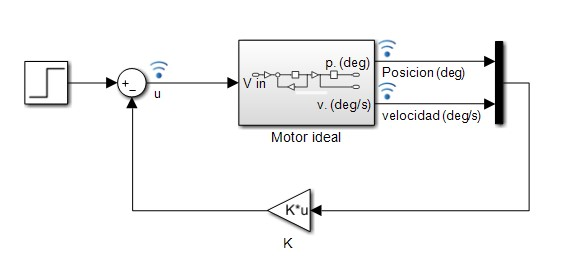
\includegraphics[width=0.5\textwidth]{r_estados.jpg}
\caption{Modelo del sistema realimentado}
\label{f31a}
\end{subfigure}
\begin{subfigure}{\textwidth}
\centering
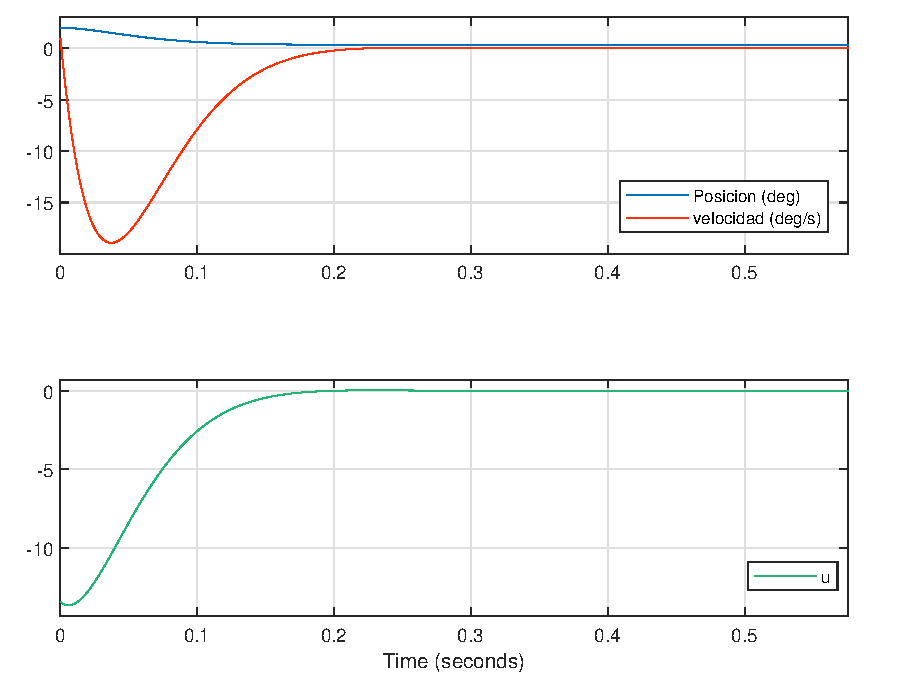
\includegraphics[scale=0.6]{r_estados.eps}
\caption{Evolución de los estados y señal de entrada al motor}
\label{f31b}
\end{subfigure}
\caption{Realimentación de estados para el motor ideal}
\end{figure}

\paragraph{Diseño de un  estimador} Como ya hemos descrito más arriba, de las dos variables de estado que definen nuestro sistema, la velocidad resulta difícil de precisar, sobre todo cuando el motor acelera o frena. Se hace por tanto necesario diseñar un sistema que emplee realimentación de estados estimados. Para diseñarlo, gracias al principio de separación, podemos calcular la ganancia $L$ del estimador, empleando de nuevo  \texttt{acker} o \texttt{place} y conservar las ganancias $K$ obtenidas para la realimentación de estados. Podemos colocar los polos del estimador a la izquierda del polo $p$ del motor, por ejemplo $p_{e1} = 1.2p$ y $p_{e2} = 1.2p $. Podemos ahora repetir la simulación, empleando la realimentación de los estados estimados en lugar de los estados reales. Para ello, añadimos al modelo de Simulink de la figura \ref{f31a} un estimador de estados, empleando de nuevo los datos obtenidos para el motor real en la práctica de identificación. El modelo completo resultante se muestra en la figura \ref{f32a}. La estructura del estimador, corresponde al modelo completo en variables de estado. Las matrices $A$, $B$, $C$ corresponden a las matrices del sistema (motor ideal), $K = [K_1,K_2]$, corresponden al vector de ganancias de la realimentación de estados, obtenidas anteriormente, y $L = [L_1,L_2]^T$ es el vector de ganancias del estimador. Es importante hacer notar que los bloques de ganancias del modelo de Simulink hay que configurarlos para que calculen productos matriciales. El modelo está construido de modo que toma todos los parámetros del sistema del \emph{work space} de Matlab. Al modelo se le ha añadido una ganancia de entrada a la que se ha dado valor $1$. Corresponde al valor de la ganancia $F_c$ de acción directa. El valor asignado es arbitrario por lo que no cabe esperar que el motor alcance la posición de consigna indicada por la entrada escalón\footnote{Para que la acción directa (\emph{{feedforward}}) llevara el motor a la posición indicada por el escalón de entrada, $y = x_r$, Es preciso ajustar el valor de $F_c$,
\begin{equation}
	F_c = (C(BK-A)^{-1}B)^{-1}
\end{equation}  
}.
La figura \ref{f32b} muestra la evolución de los estados del sistema así como la de los estados estimados, para una entrada escalón de valor 5. Puede observarse como el motor alcanza una posición final, y como los estados estimados convergen a  los reales antes de alcanzar el estado final. La convergencia es lo suficiente rápida para que el sistema siga una trayectoria muy parecida a la del caso anterior, \ref{f31b} en que se empleaba realimentación de estados reales. Lógicamente, se podría acelerar dicha convergencia, desplazando los polos del estimador más a la izquierda. Se observa también que el sistema no alcanza el valor de la entrada. Esto era de esperar puesto que no hemos ajustado el valor de la ganancia $F$, para que esto ocurra. De hecho, no vamos a calcular dicho ajuste. En su lugar, añadiremos directamente acción integral a nuestro sistema de control.

\paragraph{Acción integral} Si añadimos acción integral al sistema de control, conseguimos que el motor siga a la entrada de referencia. Debemos para ello calcular la ganancia $k_i$ correspondiente a la acción integral. Tenemos dos modos de hacerlo. Podemos colocar de nuevo los tres polos en posiciones pre-establecidas y emplear \texttt{acker} o \texttt{place} para obtener las ganancias $K = [K_1,K_2,K_i]$. Esto nos da la oportunidad de mantener los polos de la realimentación de estados en la misma posición que estaban cuando no se empleaba acción integral. Tenemos también la alternativa de conservar las ganancias calculadas previamente para la realimentación de estados y emplear la técnica del lugar de las raíces para obtener la ganancia $k_i$. Con esto tendríamos nuestro motor ideal controlado en posición. La figura \ref{f33a} muestra el controlador completo. Se ha recuadrado en rojo la parte que corresponde a la acción integral y en azul la parte que corresponde al estimador de estados.

\begin{figure}
\centering
\begin{subfigure}{\textwidth}
\centering
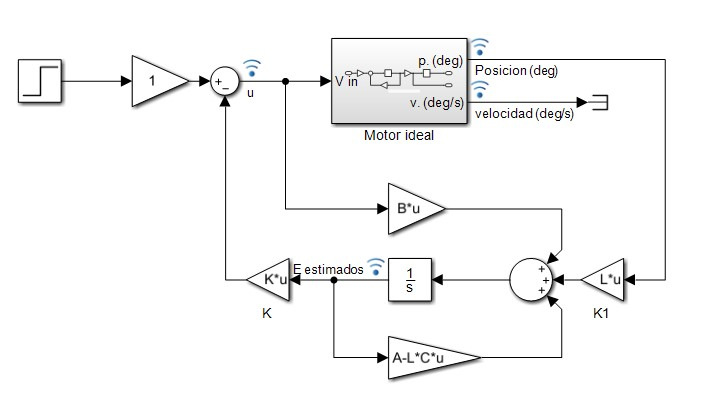
\includegraphics[width=0.5\textwidth]{estimador.jpg}
\caption{Modelo del sistema con el estimador de estados}
\label{f32a}
\end{subfigure}
\begin{subfigure}{\textwidth}
\centering
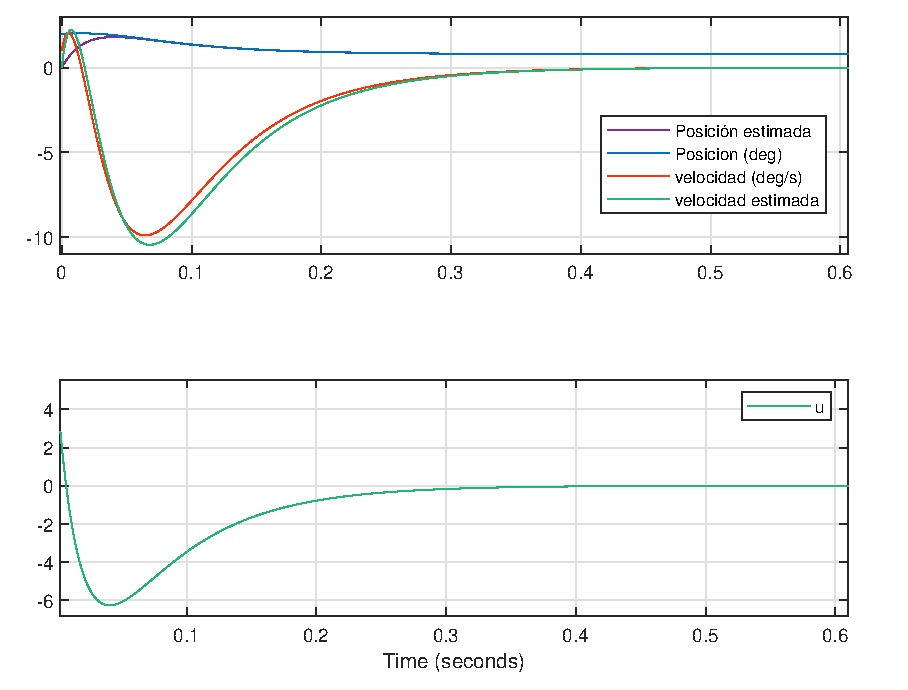
\includegraphics[scale=0.6]{estimador.eps}
\caption{Evolución de los estados y señal de entrada al motor}
\label{f32b}
\end{subfigure}
\caption{Realimentación de estados estimados para el motor ideal. La entrada es un escalón de valor 5}
\end{figure}




Para este ejemplo, se ha cambiado la posición de los polos. Así los polos del motor se han situado en $p_1 = -15, p_2 = -15$, el correspondiente al estado de la acción integral en $p_i = -20$ y los polos del observador en $p_{e,1} = -30, p_{e,2} = -30$. El modelo del motor sigue empleando $K_e = 100$ y $p = 50$. La entrada escalón sigue teniendo un valor final 5.

La figura \ref{f33b} muestra, en la gráfica superior, la evolución de los estados del sistema así como la de los estados estimados. Puede observarse como, ahora el motor sí consigue alcanzar la posición angular $5$ correspondiente al valor de referencia consignado por la entrada escalón.

En la gráfica inferior se ha representado el estado de la  acción integral $z$ junto con el valor de la entrada $u$. Es interesante notar, como el estado $z$ alcanza un valor estacionario distinto de cero, cuando el motor ha alcanzado su valor estacionario.

Hemos prestado poca atención a $u$, el valor obtenido para la señal de entrada. Es importante recordar que dicho valor corresponde al voltaje Vref con que debemos alimentar el motor.  Conviene recordar que dicho valor no puede superar el valor $V_{max}=12V$ en el sistema real. Ahora que tenemos un modelo completo, podemos estudiar el efecto de la posición de los polos ---y, por tanto, de las ganancias $K$ y $L$--- tanto en la respuesta del sistema como en los valores que alcanzará la señal de entrada $u$. 

Así mismo podemos observar también el efecto que tiene el error en posición del motor, es decir, la diferencia entre la posición angular de su eje y el valor de referencia o valor final que debe alcanzar $\theta_r-\theta(t)$.

Si el sistema de control demanda valores mayores que $V_{max}$, esto no tiene efecto alguno en el sistema ideal, pero llevará a una saturación en la entrada del sistema real. En principio esto no debería tener mayores consecuencias en el motor real, que simplemente giraría a velocidad máxima hasta acercarse lo suficiente al valor de referencia de la posición como para que la acción de control deje de saturar la entrada, a partir de ahí, disminuiría el voltaje de entrada hasta alcanzar su posición final\footnote{Esto no es completamente cierto debido a la presencia del control integral, que podría hacer que el motor oscilase. Hablaremos de ello más adelante.}.
  
\paragraph{Práctica 4}
\begin{enumerate}
\item Construir un modelo en Simulink, que incluya el motor ideal y un sistema de control por realimentación de estados estimados y acción integral. 
\item Comprobar el efecto de la posición de los polos del sistema y el estimador sobre la velocidad de respuesta del sistema y el valor de la señal de control $u$. (incrementarlos o disminuirlos en potencias de 10)
\item Comprobar el efecto de la ganancia de la alimentación directa $F_c$.
\item Observar el efecto del error de posición inicial sobre la señal de entrada $u$. 
\end{enumerate}

\begin{figure}
\centering
\begin{subfigure}{\textwidth}
\centering
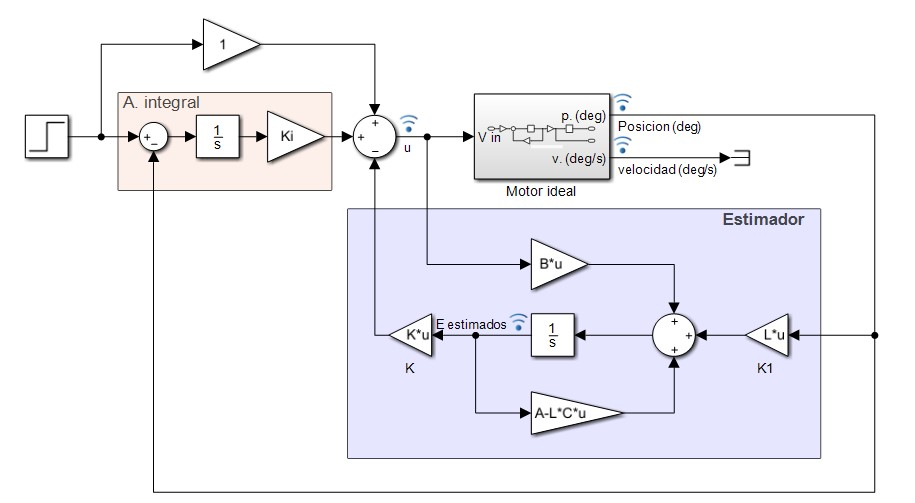
\includegraphics[width=0.5\textwidth]{estimador_integral.jpg}
\caption{Modelo del sistema con el estimador de estados}
\label{f33a}
\end{subfigure}
\begin{subfigure}{\textwidth}
\centering
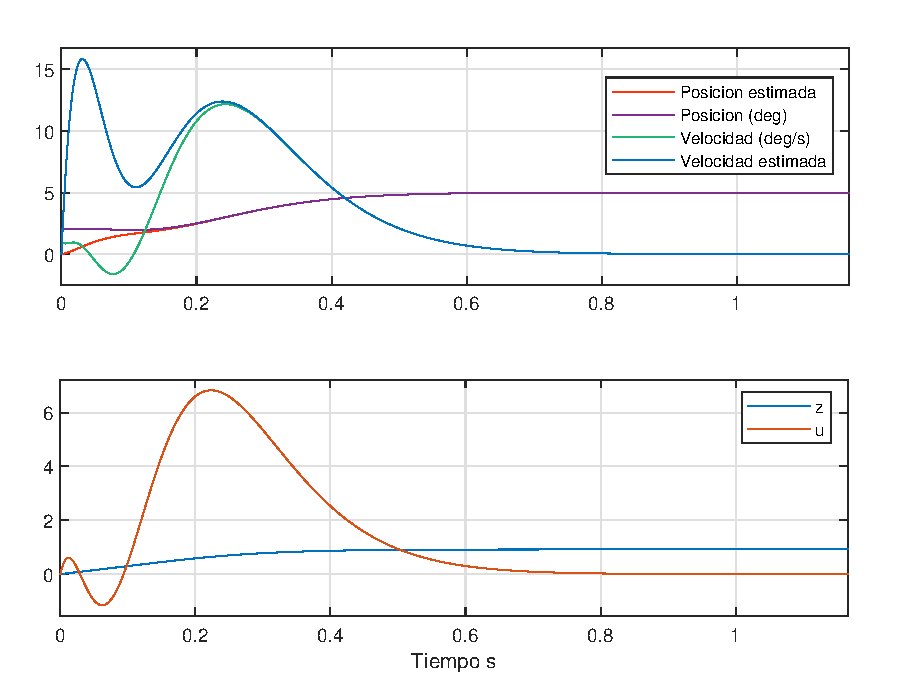
\includegraphics[scale=0.6]{estimador_integral.eps}
\caption{Evolución de los estados y señal de entrada al motor}
\label{f33b}
\end{subfigure}
\caption{Realimentación de estados estimados para el motor ideal}
\end{figure}

\subsection{Discretización del controlador para control del motor real}
Para terminar de diseñar el sistema de control, debemos tener en cuenta que el motor es controlado y observado por un sistema digital. Es decir, la señal de entrada (voltaje) que recibe el motor y la señal de salida (lectura de encoders) no se realiza de modo continuo, sino discreto.    Marcado por el periodo de muestreo al que la placa ST Nucleo envía o recibe datos por sus pines.
Podemos modelar el efecto del muestreo, empleando un retenedor de orden cero (ZOH) y un muestreador. La figura, \ref{f34a} muestra  un modelo de entrada y salida de una planta continua empleando retenedores.
La señal de entrada $u(t)$ es muestreada con un periodo de muestreo $T$.  Las muestras, que corresponden a los valores de la señal en periodos de tiempo regulares múltiplos del periodo $u(nT)$, son introducidas en el retenedor que, mantendrá el valor recibido hasta el siguiente  instante de muestreo $(n+1)T$. La salida del retenedor es una señal continua a \emph{escalones}. Un ejemplo de estas tres señales se muestra en la figura \ref{f34b}.
\begin{figure}
\centering
\begin{subfigure}{\textwidth}
\centering
\begin{circuitikz}

\draw (0,2) to[short,i=$u(t)$](0.5,2)to[cspst=T,i=$u(nT)$](3,2)to[generic=ZOH,i=$h(t)$]  (6,2)to[generic=G(s),i=$y(t)$] (9,2)to[cspst=T,i=$y(nT)$](11.5,2);
\draw(3.5,1)rectangle(10.4,3);
\node at (7,0.4){G(Z)};
\end{circuitikz}
\caption{Esquema de una planta continua y su discretización mediante el uso de un retenedor de orden cero (ZOH) y muestreadores}
\label{f34a}
\end{subfigure}
\begin{subfigure}{\textwidth}
\centering
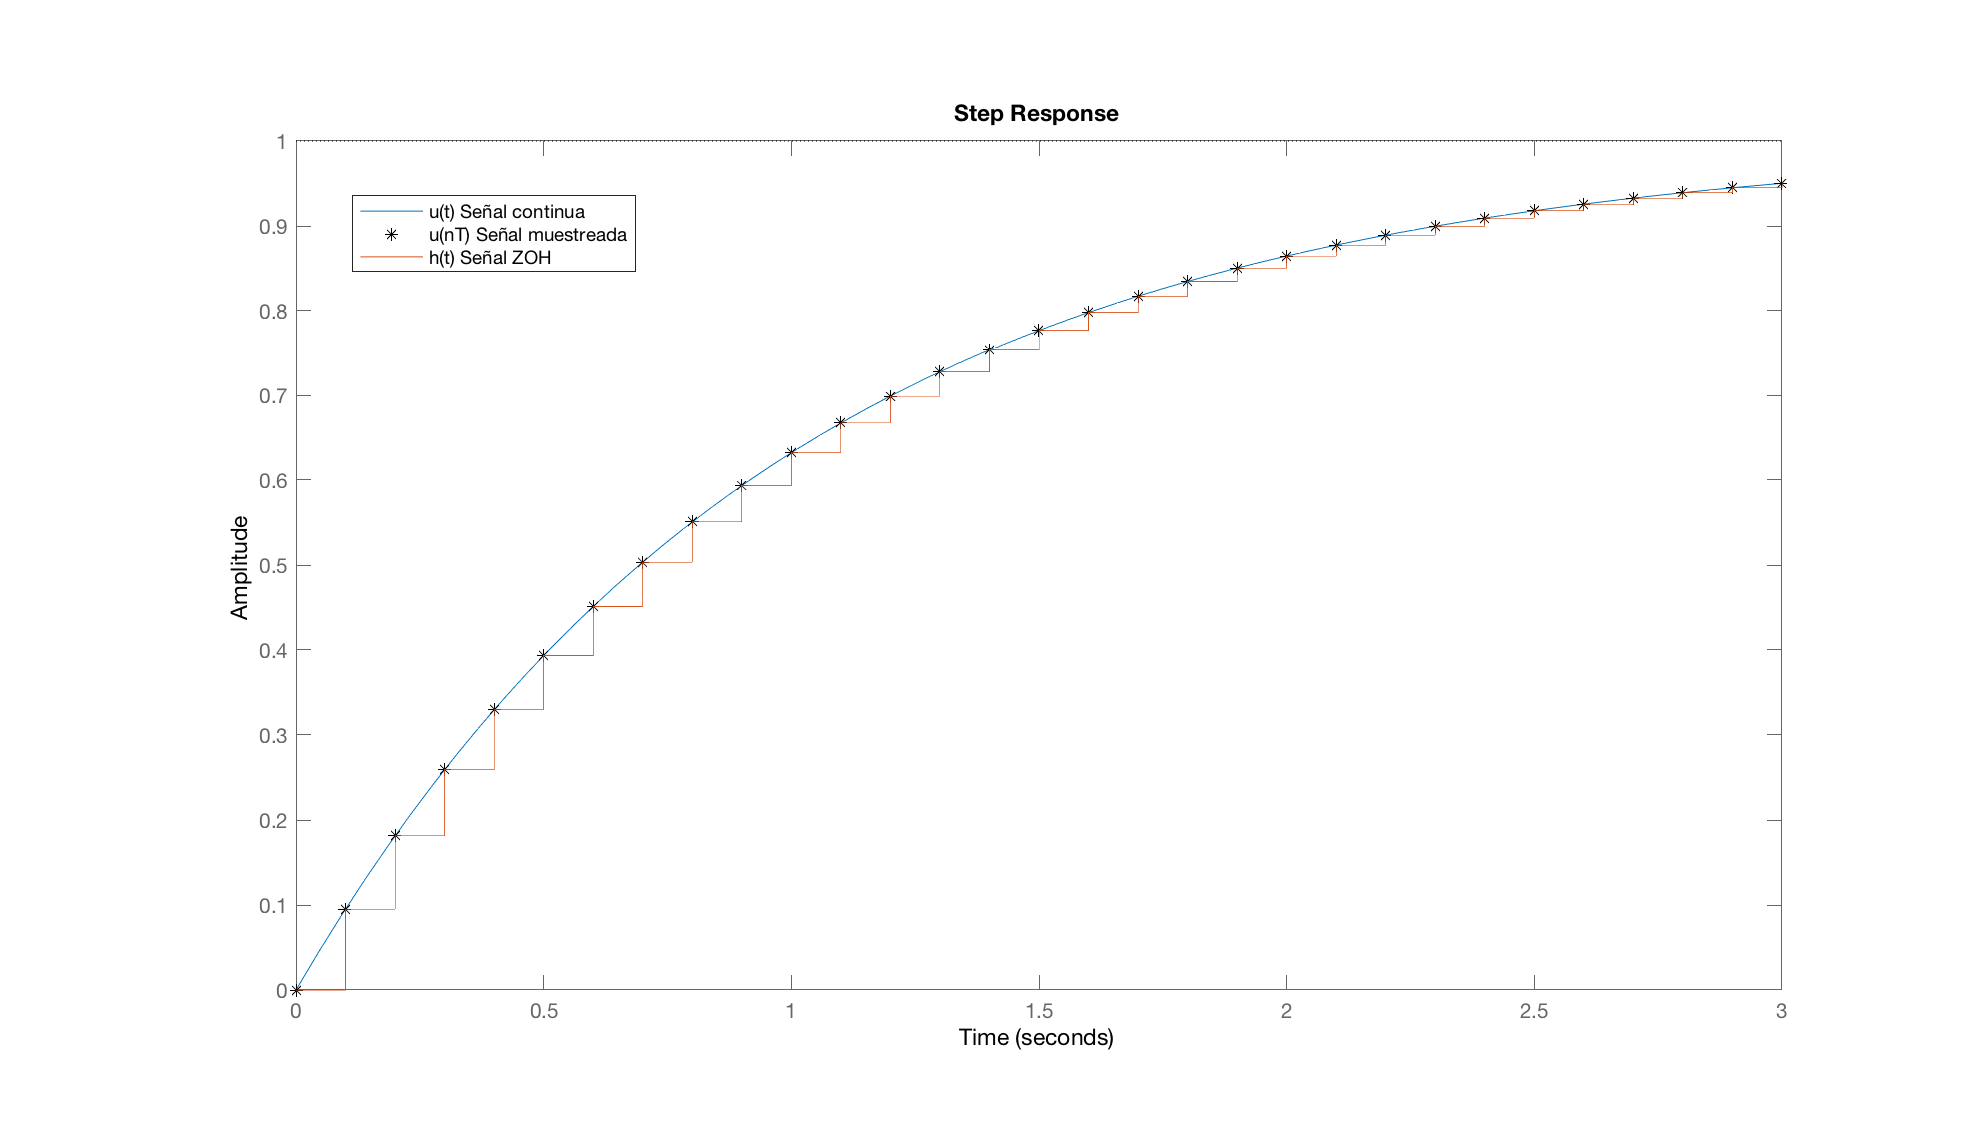
\includegraphics[width= \textwidth]{zoh.eps}
\caption{Comparación entre una señal continua $u(t)$, su versión muestreada $u(nT)$ y su aspecto $h(t)$ tras cruzar un ZOH }
\label{f34b}
\end{subfigure}
\caption{Sistema muestreador/retenedor de orden 0 (ZOH)}
\end{figure}

Si construimos en Simulink, un control en variables de estado, y lo añadimos al sistema desarrollado para manejar el motor real a traves de la placa ST Núcleo,  tenemos que tener presente por tanto, que ésta no ve al motor como un sistema continuo sino como un sistema discreto con una entrada $u(nT)$ y una salida $y(nT)$, que equivaldría a los bloques  ZOH, G(s) y el muestreador, recuadrados en la figura \ref{f34a}.

Deberíamos, por tanto obtener un modelo de la versión discreta del motor, tal y como la ve la placa.  En general, un modelo en variables de estado discreto, se define como,

 \begin{align}
\mathbf{x}(n+1) = F\mathbf{x}(n) + G\mathbf{u}(n) \label{eq42}\\
\mathbf{y}(n)  = C\mathbf{x}(n)+D\mathbf{u}(n) \label{eq43}
\end{align} 

El papel de las matrices $F$, $G$, $C$ y $D$ es análogo al de las matrices $A$, $B$, $C$ y $D$ en el caso continuo. La diferencia fundamental es que ahora las variables no son función del tiempo sino del número de muestra $n$ y que la ecuación de estados relaciona los estados en la muestra $n+1$ con los estados en la muestra $n$.

Si queremos relacionar un sistema continuo, con su versión discreta obtenida por muestreo con un periodo T, debemos considerar que los valores de las señales del sistema discreto (muestras) deben coincidir con las del sistema continuo para precisamente en los instantes de muestreo $t = nT$, es decir, $y(n) = y(t),\ \forall t = nT, n = 0,1,\cdots$ 

Para el sistema continuo sabemos que podemos expresar sus estados y su respuesta a un estado inicial $x_0$ y una entrada $u(t)$ como,
\begin{align}
x(t) &= e^{A(t-t_0)}x_0 + \int_{t_0}^t e^{A(t-\tau)}Bu(\tau)d\tau\\
y(t) &= Cx(t) + Du(t)
\end{align}

La versión discreta solo considerará los valores correspondiente a los instantes de muestreo $nT$. Supongamos que calculamos la evolución de los estados del sistema precisamente entre dos instantes de muestreo sucesivos, $t=(n+1)T$, $t_0=nT$,

\begin{align}
x((n+1)T) &= e^{AT}x(nT) + \int_{nT}^{(n+1)T} e^{A((n+1)T-\tau)}Bh(\tau)d\tau\\
y(nT) &= Cx(n) + Du(n)
\end{align}

Donde sustituimos la señal de entrada $u(t)$ por su valor tras atravesar el retenedor $h(\tau)$. Por otro lado, dados los límites de la integral, el retenedor estará dando como salida constante durante todo el periodo el valor de la variable $u$ al comienzo del mismo: $h(\tau) = u(nT)$. Como se trata de un valor constante, podemos sacarlo fuera de la integral. El resultado sería
\begin{align}
x((n+1)T) &= e^{AT}x(nT) + \left[\int_{nT}^{(n+1)T} e^{A((n+1)T-\tau)}Bd\tau\right] u(nT) \label{eq48}\\ 
y(nT) &= Cx(nT) + Du(nT) \label{eq49}
\end{align}

Sin pérdida de generalidad podemos sustituir en las definiciones de las variables $nT$ por $n$, puesto que el periodo de muestreo solo nos indica la relación de las muestras con el instante en que se tomaron. Además es fácil ver que la integral de la ecuación \ref{eq48} es precisamente la convolución sobre un periodo de la matriz de transición de estados con un escalón unitario. Por otro lado, esto no tiene nada de sorprendente puesto que el retenedor convierte la señal de entrada en escalones de duración $T$. Podemos, por tanto, calcular la integral para un periodo,
\begin{equation}
\int_{nT}^{(n+1)T} e^{A((n+1)T-\tau)}Bd\tau = \int_0^Te^{A(T-\tau)}Bd\tau = e^{AT}\left[\int_0^Te^{-A\tau}d\tau \right]Bu(n)
\end{equation}

Podemos reescribir las ecuaciones \ref{eq48}, \ref{eq49} como,
\begin{align}
x(n+1) &= e^{AT}x(n) + e^{AT}e^{AT}\left[\int_0^Te^{-A\tau}d\tau \right]Bu(n) \label{eq411}\\
y(n) &= Cx(n) + Du(n) \label{eq411}
\end{align}

Podemos  ahora relacionar los resultados obtenidos con los valores de las matrices $F$, $G$, $C$ y $D$ del sistema en variables de estado discreto (ecuaciones \ref{eq42} y \ref{eq43}), 
\begin{align}
F = e^{AT} & \ G = e^{AT}\left[\int_0^Te^{-A\tau}d\tau \right]B\\
C = C\ \ \  & \ D=D
\end{align}

Si la matriz $A$ es invertible, podemos calcular directamente la integral de la expresión para $G$,

\begin{equation*}
	G = e^{AT}A^{-1}\left[I-e^{-AT}\right]B
\end{equation*}

En nuestro caso $A$ es una matriz defectiva, pero eso hace fácil el cálculo de su exponencial:

\begin{equation*}
	e^{-A\tau}=\exp\left(-\begin{bmatrix}
		0 & 1\\
		0 &-p
	\end{bmatrix}\tau\right) = \begin{bmatrix}
	1 & -(e^{p\tau}-1)/p\\
	0& e^{p\tau}
\end{bmatrix}
\end{equation*}
Si calculamos la integral entre $0$ y $T$,
\begin{equation*}
	\int_0^Te^{-A\tau}d\tau = 
	\begin{bmatrix}
		T & Tp-e^{Tp}+1)/p^2\\
		0 &(e^{Tp}-1)/p
	\end{bmatrix}
\end{equation*}
Obtenemos finalmente,

\begin{equation}
	G = e^{AT}\begin{bmatrix}
		T & Tp-e^{Tp}+1)/p^2\\
		0 &(e^{Tp}-1)/p
	\end{bmatrix}B
\end{equation}



Para controlar el motor real empleando realimentación de estados estimados, debemos sustituir el estimador continuo por su versión discreta, calculando los valores de las matrices $F$ y $G$ a partir de los valores de las matrices $A$ y $B$ y del periodo de muestreo $T$. Matlab suministra el comando \texttt{c2d} que obtiene directamente la versión muestreada de un sistema continuo definido en variables de estado mediante el comando \texttt{ss}. Así si el sistema continuo es: \texttt{sys = ss(A,B,C,D)} el discreto correspondiente para un periodo de muestreo T se obtiene como : \texttt{sysd = c2d(sys,T)}.

 

\paragraph{Discretización de los polos} Debemos recalcular los valores de las ganancias K y L para emplearlos con el estimador discreto. Para ello, podemos trasladar los polos de continuo a discreto. Supongamos que queremos para el sistema continuo un polo de valor $\lambda_i$. Sabemos que la respuesta asociada a este polo está relacionada con una función exponencial, si muestreamos dicha respuesta:
\begin{align}
&y(t) \approx e^{\lambda_it} \rightarrow y(nT) \approx e^{\lambda_inT} \rightarrow y(n) \approx \left(e^{\lambda_iT}\right)^n\\
&\lambda_i \rightarrow  \Lambda_i = e^{\lambda_iT} \label{eq416}
\end{align}

Por tanto, podemos obtener los polos del sistema discreto (muestreado) $\Lambda_i$ a partir de los polos del sistema continuo $\lambda_i$ y el tiempo de muestreo $T$. Es interesante notar cómo el carácter estable o inestable del sistema no cambia al discretizarlo, si $re\{\lambda_i\} \le 0$ entonces $|\Lambda_i| < 1$ que corresponde con la condición de estabilidad de un sistema discreto $\Lambda_i \le 1 \Rightarrow  \lim_{n\rightarrow \infty} \Lambda_i^n =0$.

Las ganancias $K$ y $L$ para el sistema discreto pueden obtenerse, igual que el caso continuo empleando \texttt{acker} o \texttt{place}: Se diseñan la posición de los polos para la planta $\lambda_{pi}$ y el observador $\lambda_{oi}$, se discretizan empleando la ecuación \ref{eq416} y se introducen en \texttt{acker} junto con las matrices del sistema discretizado:
\begin{align*}
K &= \text{acker}(F,G,[\Lambda_{p1}...\Lambda_{pn}])\\
L &= \left(\text{acker}(F^T,C^T,[\Lambda_{o1}...\Lambda_{on}])\right)^T
\end{align*}

\paragraph{Discretización de la acción integral.} Debemos también discretizar la acción integral para incluirla en el controlador del motor. Si partimos de la ecuación de estado para la acción integral y la discretizamos,
\begin{align*}
\dot{z}(t) = C \mathbf{x}(t) - x_r \rightarrow \frac{z(n+1)-z(n)}{T}= C \mathbf{x}(n) - x_r \rightarrow z(n+1) = z(n) +TC  \mathbf{x}(n) +Tx_r
\end{align*}

Podemos emplear esta última ecuación directamente para construir el sistema ampliado,

\begin{align}
\begin{bmatrix}
\mathbf{x}(n+1)\\
z(n+1)
\end{bmatrix} &= \begin{bmatrix}
F & 0\\
TC & 1
\end{bmatrix}\cdot\begin{bmatrix}
\mathbf{x}(n)\\
z(n)
\end{bmatrix}+\begin{bmatrix}
G\\
0
\end{bmatrix}u(n) + \begin{bmatrix}
0\\
-T
\end{bmatrix}x_r
\end{align}  

Podemos directamente emplear el sistema ampliado con la acción integral discreta para recalcular los valores de las ganancias $[K,k_i]$ empleando el mismo método descrito en el párrafo anterior.

\paragraph{Acción Directa} Una última nota para el cálculo de la acción directa para el sistema muestreado. Hemos omitido su cálculo hasta ahora ya que si empleamos acción integral podemos asignarle un valor arbitrario (aunque razonable). Vamos de todos modos a recordar la expresión de la acción directa para un sistema continuo y como adaptarla para una versión discretizada dicho sistema. Si llamamos $f$ a al valor de la ganancia de la acción directa necesaria para que la planta alcance el estado estacionario tendremos que,
\begin{align}
&\mathbf{x_{ssD}} = (F -GK)\mathbf{x_{ssD}} + Gfx_r\\
&\left[I-(F-GK) \right]\mathbf{x_{ssD}} =Gfx_r\\
&\mathbf{x_{ssD}} = \left[I-(F-GK) \right]^{-1}Gfx_r\\
&y_{ssD} = C\mathbf{x_{ssD}} = x_r, (D = 0)\\
&x_r = C\left[I-(F-GK) \right]^{-1}Gfx_r\\
&C\left[I-(F-GK) \right]^{-1}Gf = I\\
&f = \left[C\left[I-(F-GK) \right]^{-1}G\right]^{-1}
\end{align}

Es interesante observar que el resultado no coincide con el cálculo de la ganancia $F_c$ para el caso continuo. De hecho, ambos sistemas continuo y discretizado, alcanzarán el mismo valor de consigna pero por caminos distintos. 

Si se emplea acción integral, es posible elegir libremente tanto $F_c$ como $f$. Se puede entonces ajustar el valor de $f$ para que las trayectorias de ambos sistemas coincidan. Así para valores dados de $F_c$ y $f$, sabemos que,
\begin{align}
y_{ss}  &= -C\left[A-BK\right]^{-1}BF_cx_r\\
y_{ssD} &= C\left[I-(F-GK) \right]^{-1}Gfx_r
\end{align}
Buscamos asegurar que ambos valores (continuo y discretizado) en estacionario sean iguales $Y_{ss} = Y_{ssD}$ Si igualamos la expresiones de los estados estacionarios y despejamos $f$
\begin{align}
-C\left[A-BK\right]^{-1}BF_cx_r = C\left[I-(F-GK) \right]^{-1}Gfx_r\\
f = -\left[C\left[I-(F-GK) \right]^{-1}G\right]^{-1}C\left[A-BK\right]^{-1}BF_c  \\\label{eq429}
\end{align}
Obtenemos una relación entre $f$ y $F_c$

\paragraph{Práctica 5}
\begin{enumerate}
\item Diseñar un sistema de control basado en realimentación de estados para el motor, empleando los parámetros $K_e$ y $p$ identificados en la práctica 2.
\item Estudiar el efecto de la posición de los polos y los valores de $f$ en la respuesta obtenida para entradas escalón. Examinar el efecto sobre la entrada del sistema $u$. 
\end{enumerate}

\begin{figure}
\centering
\begin{subfigure}{0.6\textwidth}
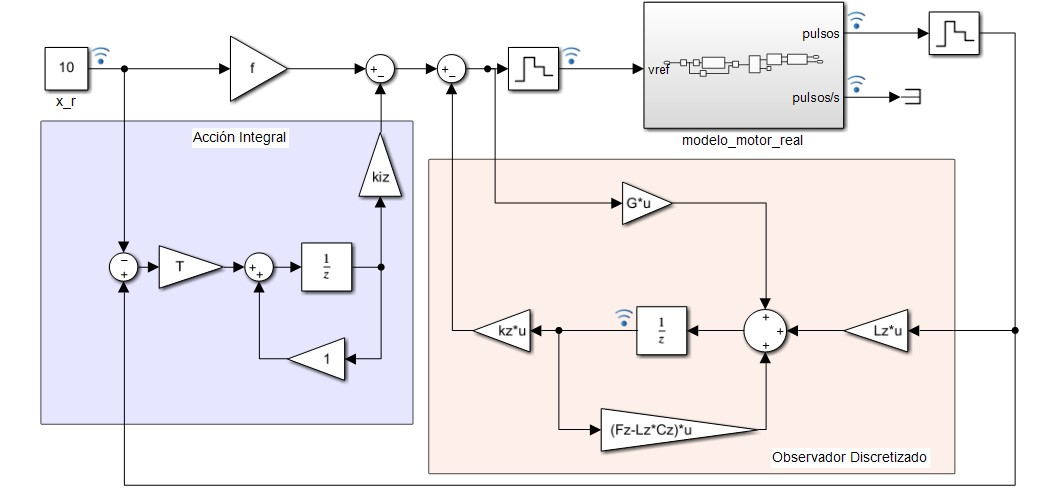
\includegraphics[width=\textwidth]{motor_controlado.jpg}
\caption{Modelo de motor completo con control discretizado}
\label{f35a}
\end{subfigure}
\begin{subfigure}{0.6\textwidth}
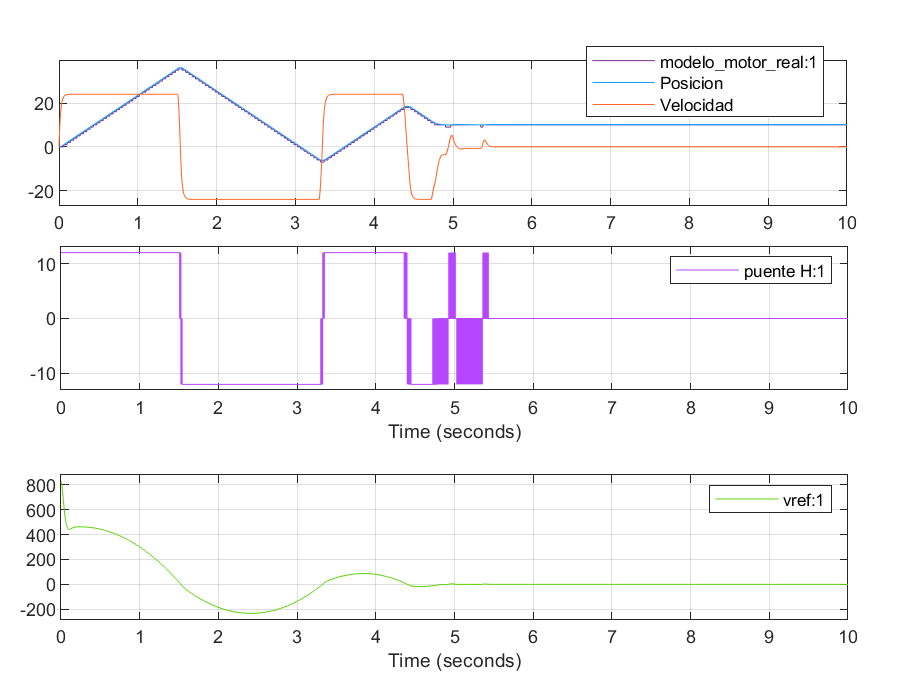
\includegraphics[width=\textwidth]{motor_controlado.eps}
\caption{Respuesta del sistema $f$ calculado a partir de $F$}
\label{f35b}
\end{subfigure}
\begin{subfigure}{0.6\textwidth}
\includegraphics[width=\textwidth]{motor_controlado_f0.eps}
\caption{Respuesta del sistema $f=0$}
\label{f35c}
\end{subfigure}
\caption{Modelo completo del motor con control discretizado por realimentación de estados estimados, acción integral y acción directa}
\end{figure}
\section{Controlador discreto para el modelo completo del motor y el motor real}

Finalmente, podemos construir un modelo de Simulink que incluya el modelo del motor desarrollado en la sección \ref{sec41} y el controlador discretizado que acabamos de describir en la sección anterior. 

La figura \ref{f35a} muestra el modelo completo. 

El bloque marcado como \texttt{modelo\_motor\_real} contiene el modelo del motor completo (ver figura \ref{f29a}) a la entrada y salida del bloque, se han añadido un par de bloques ZOH para modelar el muestreado del sistema de adquisición y control propio de la placa ST Nucleo. Recuadrado en rojo aparecen los bloques correspondientes al modelo de motor discretizado, con el que se ha construido el estimador. El bloque marcado en azul corresponde a la acción integral discretizada. 

La figure \ref{f35b} muestra la respuesta del sistema con los siguiente parámetros: 
\begin{itemize}
\item Los parámetros del motor se han fijado como $K_e = 100$ y $p =50$
\item Los polos del sistema continuo se han seleccionado como:
\begin{enumerate}
\item $P = [-15 -15 -20]$. Polos para realimentación de estados, el ultimo corresponde a la acción integral
\item $PL = [-30 -30]$.  Polos para la realimentación del error  de la salida para el estimador estimador 
\end{enumerate}
\item $F_c$ calculada para asegurar que el sistema alcanza el valor de referencia $F_c = (C(BK-A)^{-1}B)^{-1}$. (aunque no sería necesario). 
\item Tiempo de muestreo $T=0.0001s$
\item $x_r = 10^o$
\item Todos los parámetros correspondientes al sistema discretizado se han obtenido a partir de las ecuaciones descritas en la sección anterior $f$ se ha calculado a partir de $F$ empleando la ecuación \ref{eq429}.
\end{itemize}

Si observamos la salida del sistema (fig. \ref{f35b}) vemos que el motor alcanza la posición final tras realizar un par de oscilaciones amplias. Lo que no corresponde con el resultado que obtendríamos si empleáramos un modelo ideal del motor. La razón la podemos obtener comparando el gráfico en que se representa la variable $vref$, ---que corresponde al valor de voltaje de entrada calculado por el sistema de control---  con  el gráfico en que se representa la variable $puente H:1$ que nos da el voltaje real suministrado por el puente en H del modelo. El puente solo puede suministrar un voltaje máximo de $12V$, sin embargo, el controlador demanda un voltaje inicial mucho más alto. El resultado es que el motor recibe un voltaje constante de 12 V durante los primeros 1.5s. Además la posición supera con mucho el voltaje de consigna. La razón de esta sobreoscilación tan grande, se debe a la acción integral: su contribución al error crece durante mucho más tiempo del que sería deseable, ya que el motor, alimentado con $12$ voltios, avanza mucho más despacio de lo previsto, y el error integral sigue creciendo mientras el error no es cero. Cuando se alcanza el valor de referencia, la acción integral sigue obligando al motor a avanzar en la misma dirección hasta que cambia el signo de la integral. Es fácil ver que el efecto resultante ---conocido como \emph{wind-up} de la acción integral, genera una oscilización innecesaria en el sistema que, para ciertos valores de los parámetros (posiciones de los polos y valor de $f$) podría llegar a desestabilizarlo.

Para paliar en parte este efecto, una primera solución es eliminar la acción directa $f=0$. La figura \ref{f35c} muestra los resultados obtenidos, para el mismo caso anterior pero eliminando la acción directa. Es claro como ahora el sistema se estabiliza antes y se reducen las oscilaciones.

\begin{figure}
\centering
\begin{subfigure}{0.6\textwidth}
\includegraphics[width=\textwidth]{antiwindup.jpg}
\caption{Modelo de motor completo con control discretizadoy anti wind-up}
\label{f36a}
\end{subfigure}
\begin{subfigure}{0.6\textwidth}
\includegraphics[width=\textwidth]{antiwindup.eps}
\caption{Respuesta del sistema $f$ calculado a partir de $F$}
\label{f36b}
\end{subfigure}
\caption{Modelo completo del motor con control discretizado por realimentación de estados estimados, acción integral, acción directa y Anti wind-up.}
\end{figure}
\paragraph{\emph{Anti wind-up}}
Una solución más robusta a los problemas de \emph{Wind-up}, consiste en desconectar o atenuar la acción integral mientras el actuador esta saturado, es decir mientras el valor de la entrada demandado por el controlador supera el valor que éste puede dar. La figura \ref{f36a} muestra una posible construcción de dicho mecanismo, remarcado en color rosa. En este caso, no se desconecta la acción integral, sino que se altera la entrada del error de posición al integrador añadiendo un nuevo término proporcional a la diferencia entre la entrada $u$ calculada por el controlador y valor máximo de la salida. El valor de la constante de proporcionalidad ---$kamp$ en la figura--- se ajusta habitualmente en función de las características que se quieran dar a la salida. 

\begin{figure}
	\centering
		\includegraphics[width=\textwidth]{ctrlreal.jpg}
	\caption{Sistema completo para alimentar el motor real, empleando el esquema de Simulink (fig. \ref{f18}) para manejar el motor real. Los bloques añadidos antes del motor permiten pasar de tensión en voltios a señal de PWM}\label{f37}
\end{figure}
\paragraph{Práctica6}
\begin{enumerate}
\item  Construir los bloques de Simulink del estimador acción directa y  acción integral discreta y añadirlos al modelo de motor completo desarrollado en la práctica 3.
 \item Estudiar la respuesta del sistema para los sistemas de control diseñados en la práctica 5. Comprobar el efecto de eliminar la acción integral $K_iz=0$ o la acción directa $f=0$
 \item Añadir al modelo un bloque anti wind-up, analizar la salida para distintos valores de la constante $kamp$.
\item Trasladar los bloques del sistema de control desarrollado al esquema de Simulink empleado para manejar el motor real (fig \ref{f37}). Comprobar que es capaz de mover el motor desde una posición inicial $\theta_0 = 0$ hasta una posición final de referencia $\theta_r$
\end{enumerate}


%%%%%%%%%%%%%%%%%%%%%%%%%%%%%%%%%%%%%%%%%%%%%%%%%%%%%%%%%
\bibliographystyle{plain}
\bibliography{./Documentacion/practica}{}

\end{document}